\chapter{Elements}
\label{chap:elements}

Elements define how the displacement field is interpolated between nodes and therefore determine the kinematic approximation used by the finite-element model. The element formulation controls which deformation modes can be represented, how strains and curvatures are evaluated, how numerical integration is performed, and which result quantities can be recovered. Choosing an appropriate element family is therefore as important as choosing a sufficiently fine mesh.

This chapter documents the element formulations that are currently accepted by FEMaster. It is intentionally more detailed than the \cmd{ELEMENT} keyword page in Chapter~\ref{chap:model-definition}: the keyword page explains how elements are entered, while this chapter explains what the individual formulations represent, how they behave numerically, and when they should be used.

Element IDs are non-negative user labels and may start at \val{0}. Connectivity order is significant. It determines the reference orientation, element faces, shell normals, and the mapping between the reference element and the physical geometry. Always preserve the documented node order when importing or generating meshes.

\section{Supported element types}

\begin{longtable}{@{}p{0.17\linewidth}p{0.11\linewidth}p{0.61\linewidth}@{}}
\toprule
\textbf{FEMaster type} & \textbf{Nodes} & \textbf{Formulation} \\
\midrule
\endhead
\val{C3D4} & 4 & Linear tetrahedral solid. \\
\val{C3D5} & 5 & Five-node pyramid input represented by a degenerated hexahedral topology. \\
\val{C3D6} & 6 & Linear wedge solid. \\
\val{C3D8} & 8 & Linear fully integrated hexahedral solid. \\
\val{C3D8R} & 8 & Reduced-integration hexahedral solid with hourglass stabilization. \\
\val{C3D10} & 10 & Quadratic tetrahedral solid. \\
\val{C3D15} & 15 & Quadratic wedge solid. \\
\val{C3D20} & 20 & Quadratic hexahedral solid with full stiffness integration. \\
\val{C3D20R} & 20 & Quadratic hexahedral solid with reduced stiffness integration. \\
\val{S3} & 3 & Legacy three-node triangular shell. \\
\val{S4} & 4 & Legacy four-node quadrilateral shell. \\
\val{MITC4} & 4 & Legacy four-node MITC shell with tied transverse shear interpolation. \\
\val{S6} & 6 & Legacy six-node quadratic triangular shell. \\
\val{S8} & 8 & Legacy eight-node quadratic quadrilateral shell. \\
\val{MITC8} & 8 & Legacy eight-node MITC shell with tied transverse shear interpolation. \\
\val{MITC3FRT} & 3 & Three-node finite-rotation shell. \\
\val{MITC4FRT} & 4 & Four-node finite-rotation MITC shell. \\
\val{MITC6FRT} & 6 & Six-node finite-rotation MITC shell. \\
\val{MITC8FRT} & 8 & Eight-node finite-rotation MITC shell. \\
\val{QSPT} & 4 & Specialized quadrilateral shear-panel element. \\
\val{B33} & 2 & Three-dimensional beam element. \\
\val{T3} & 2 & Three-dimensional truss element. \\
\bottomrule
\end{longtable}

The Abaqus reader accepts the same solid names \val{C3D4}, \val{C3D5}, \val{C3D6}, \val{C3D8}, \val{C3D8R}, \val{C3D10}, \val{C3D15}, \val{C3D20}, and \val{C3D20R}. Abaqus \val{T3D2} is mapped to FEMaster \val{T3}. Abaqus \val{B33} is mapped to FEMaster \val{B33}. Abaqus shell names are translated as shown below.

\begin{table}[H]
\centering
\begin{tabular}{@{}lll@{}}
\toprule
\textbf{Abaqus input} & \textbf{FEMaster formulation} & \textbf{Comment} \\
\midrule
\val{S3}, \val{S3R} & \val{MITC3FRT} & Both imported labels use the finite-rotation triangular shell. \\
\val{S4}, \val{S4R} & \val{MITC4FRT} & Both imported labels use the finite-rotation four-node MITC shell. \\
\val{S6}, \val{S6R} & \val{MITC6FRT} & Both imported labels use the finite-rotation six-node shell. \\
\val{S8}, \val{S8R} & \val{MITC8FRT} & Both imported labels use the finite-rotation eight-node shell. \\
\bottomrule
\end{tabular}
\caption{Current Abaqus shell-type mapping.}
\end{table}

This mapping is important: an Abaqus \val{S4} deck does \emph{not} select the native legacy \val{S4} formulation. It is translated to \val{MITC4FRT}. Native FEMaster input can still select the legacy shell names explicitly for comparison and regression work.

\section{Solid elements}

Solid elements model a three-dimensional continuum. They use translational nodal degrees of freedom and obtain their constitutive response from a \cmd{SOLID SECTION}. They are appropriate when the full three-dimensional stress state matters, when through-thickness stresses are required, or when local geometry and load introduction cannot be represented adequately by shells or line elements.

Low-order solids are inexpensive but may require significant refinement in bending-dominated problems. Higher-order solids generally represent curvature and stress gradients more efficiently, but they contain more degrees of freedom per element and are more sensitive to poor midside-node placement and distorted mappings. Mesh quality remains essential for every formulation.

\clearpage
\section{\val{C3D4}: 4-node tetrahedral solid}

\begin{figure}[H]
    \centering
    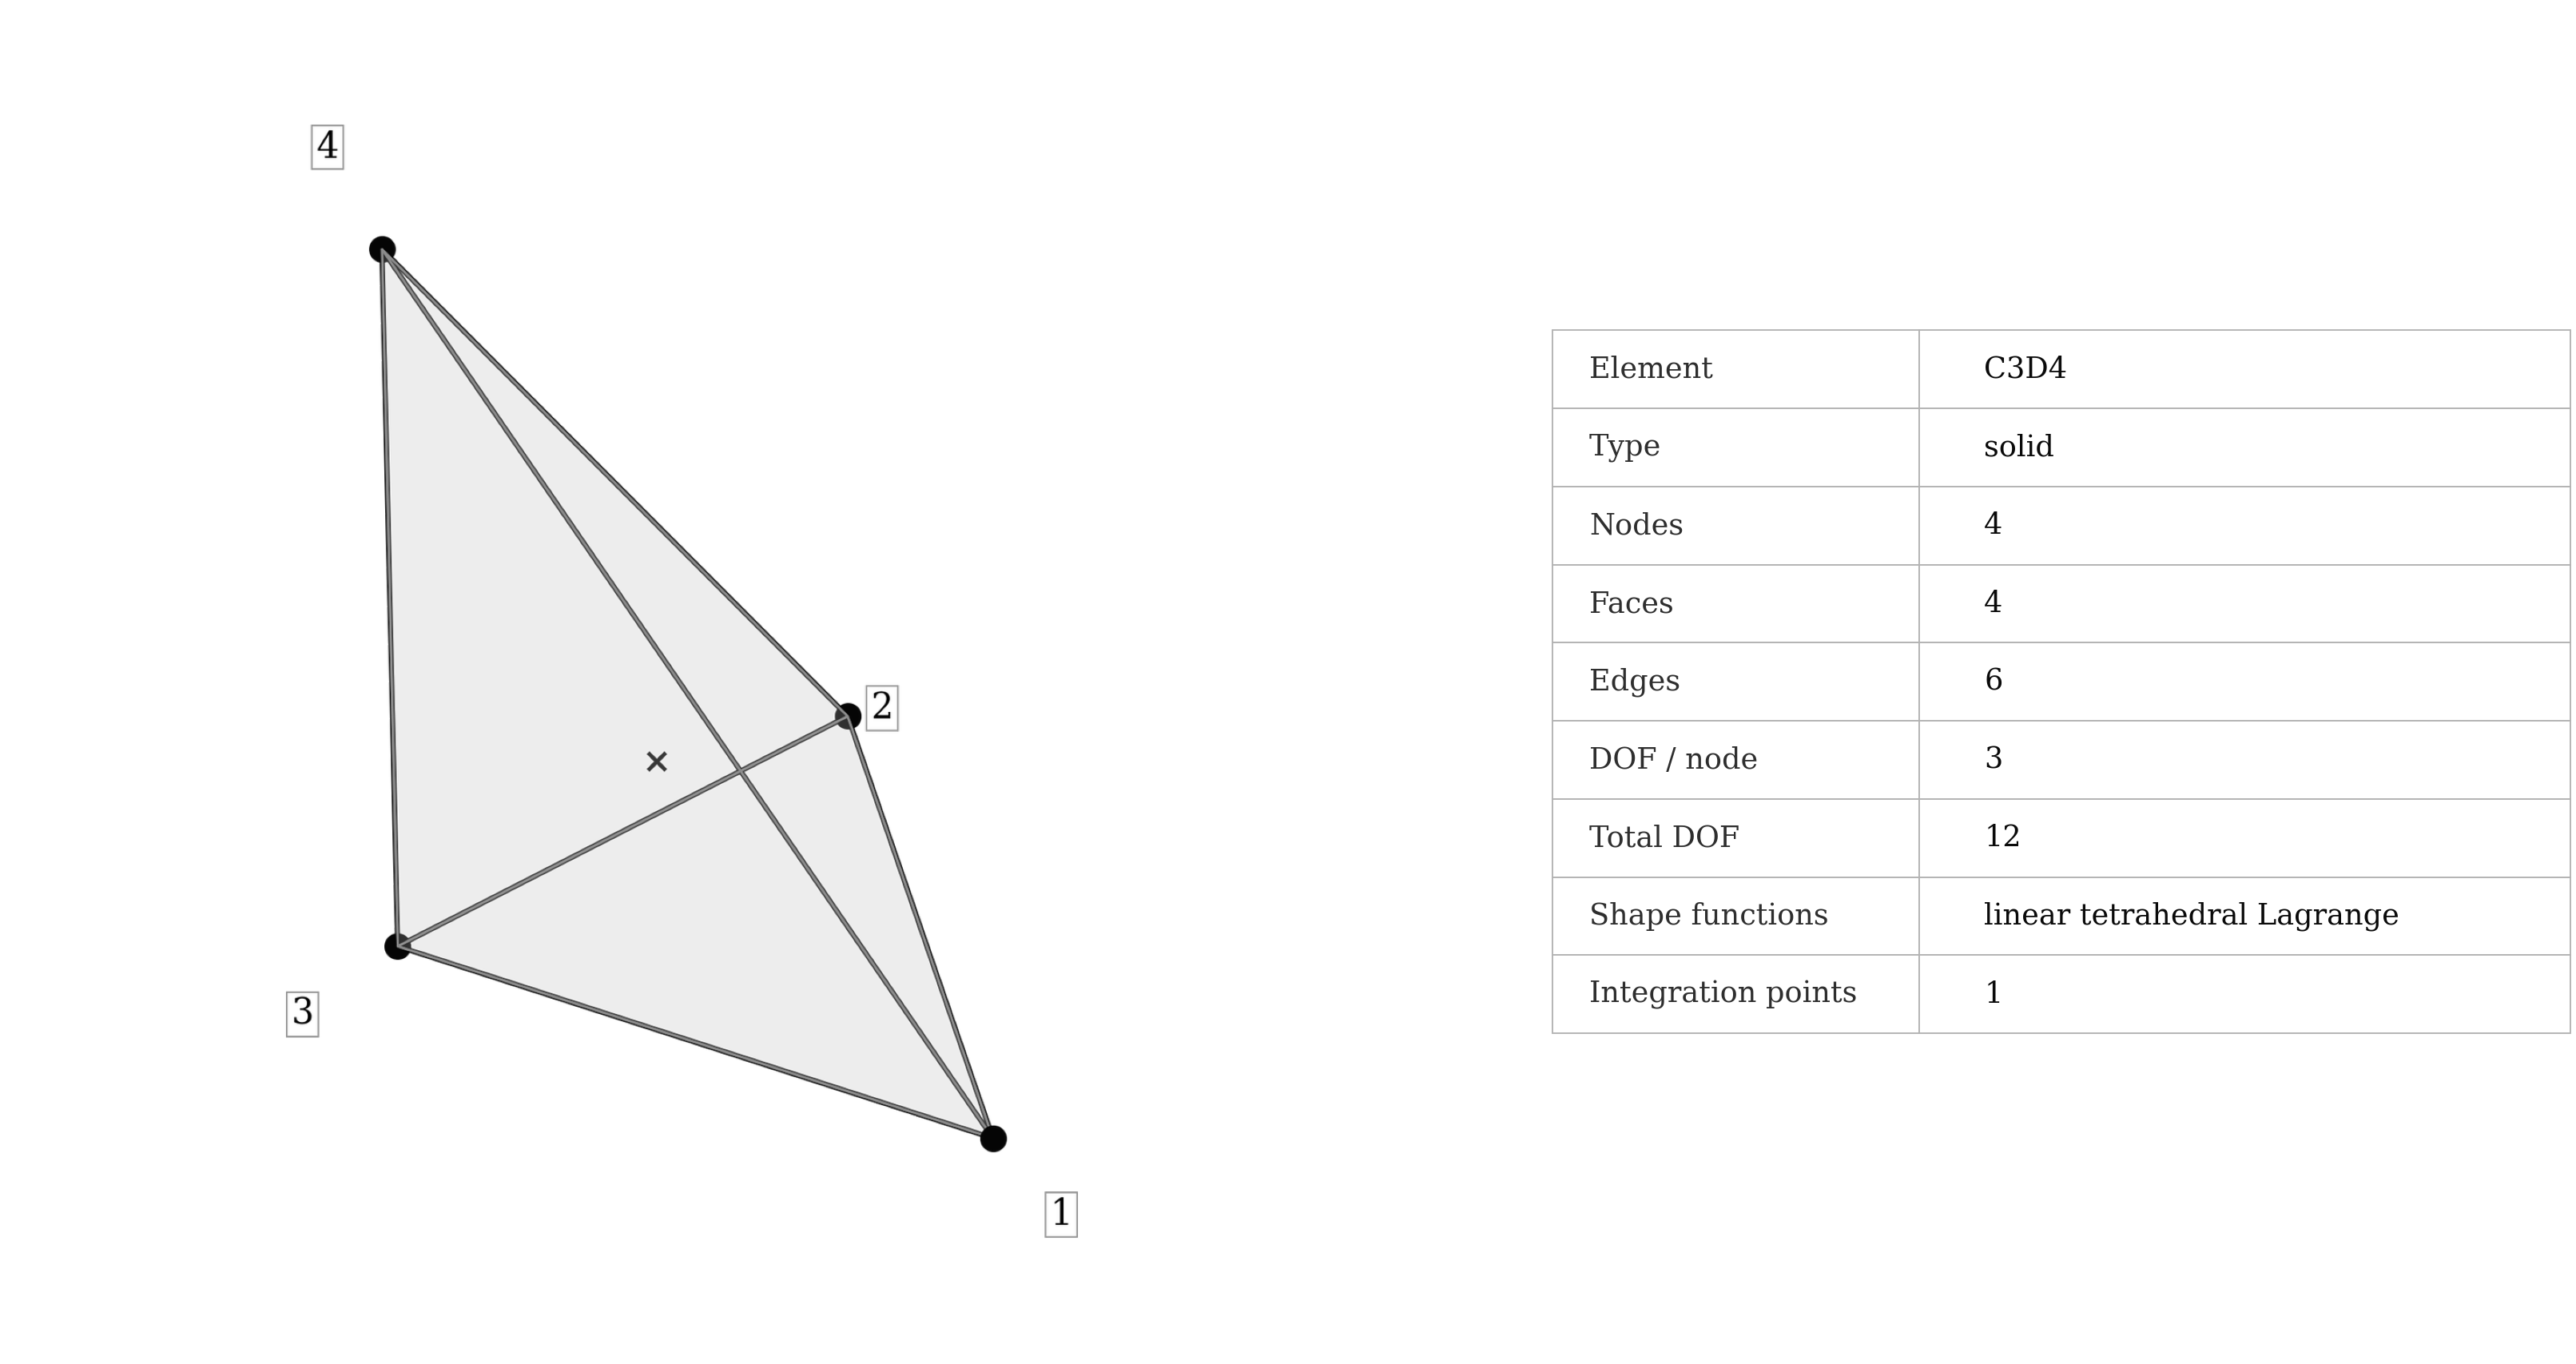
\includegraphics[width=0.78\linewidth]{pages/figures/element_schematics/c3d4_schematic.png}
    \caption{\val{C3D4} element topology and integration scheme.}
\end{figure}

\begin{syntax}
*ELEMENT, TYPE=C3D4, ELSET=<set>
<id>, <n1>, <n2>, <n3>, <n4>
\end{syntax}

\val{C3D4} is the simplest three-dimensional continuum element in FEMaster. It uses four corner nodes and linear displacement interpolation over a tetrahedral reference domain. The resulting strain field is constant within one element, which makes the element inexpensive and geometrically easy to mesh but limits the deformation and stress gradients that a single element can reproduce.

The principal advantage of \val{C3D4} is meshing flexibility. Tetrahedra can fill complex CAD volumes, narrow transitions, and irregular local details with little manual topology design. This makes \val{C3D4} useful for early stiffness checks, coarse load-path studies, and models where robust automatic meshing is more important than stress accuracy per degree of freedom.

The limitation is stiffness and stress resolution. Linear tetrahedra tend to be overly stiff in bending-dominated problems unless the mesh is fine. Since the strain state is constant in each element, stress fields can appear piecewise constant or patchy and steep gradients near holes, fillets, notches, and concentrated loads require substantial refinement.

For stress-sensitive tetrahedral models, \val{C3D10} is usually the better choice. If \val{C3D4} is used, check convergence of displacements, reactions, strain energy, and relevant averaged stresses rather than relying on a single coarse local peak.

\clearpage
\section{\val{C3D5}: 5-node pyramid input}

\begin{figure}[H]
    \centering
    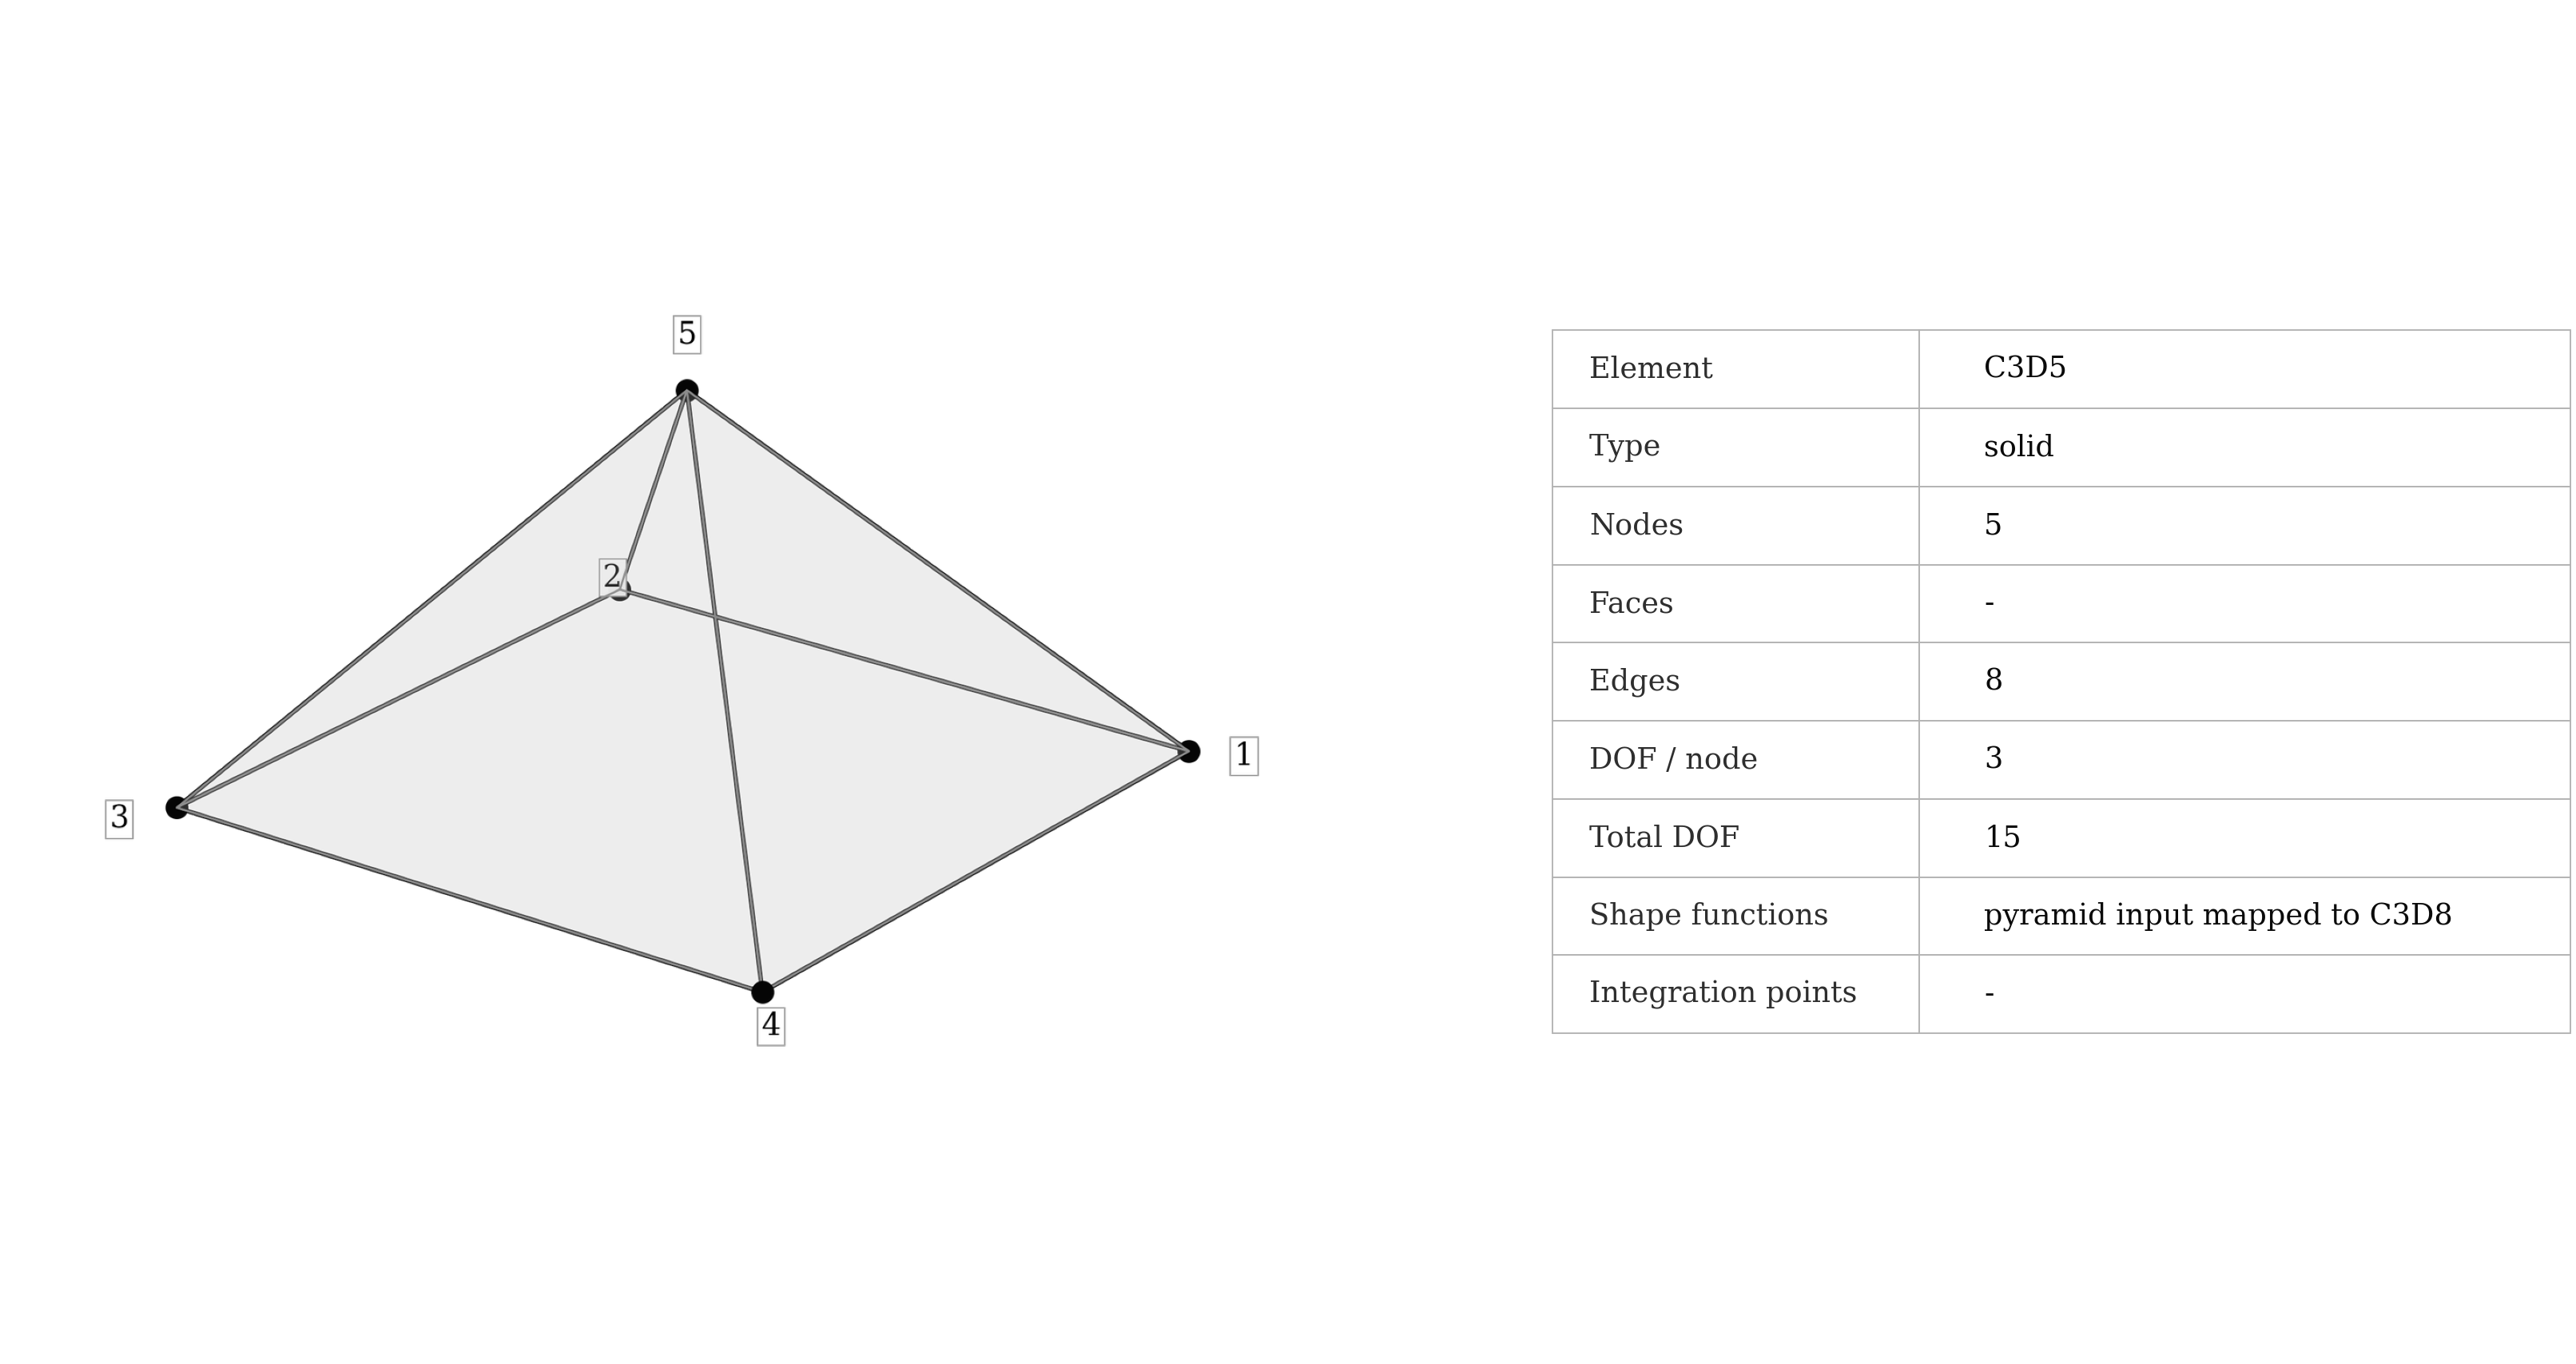
\includegraphics[width=0.78\linewidth]{pages/figures/element_schematics/c3d5_schematic.png}
    \caption{\val{C3D5} pyramid input topology.}
\end{figure}

\begin{syntax}
*ELEMENT, TYPE=C3D5, ELSET=<set>
<id>, <n1>, <n2>, <n3>, <n4>, <apex>
\end{syntax}

\val{C3D5} provides a five-node pyramid connectivity for transition meshes. FEMaster represents this input with a degenerated eight-node hexahedral topology in which the four upper hexahedral positions coincide at the pyramid apex. The user nevertheless writes the natural five-node pyramid connectivity shown above.

The element is primarily useful as a transition cell between hexahedral and tetrahedral regions. This is common in automatically generated mixed meshes where a quadrilateral face must transition toward tetrahedral topology. In such cases a small number of pyramids can preserve mesh compatibility without forcing a large surrounding region to change element family.

A degenerated mapping is generally less predictable than a regular hexahedron, wedge, or tetrahedron. Flat pyramids, badly skewed bases, and apex positions close to the base plane can produce poor Jacobians and unreliable stiffness. Treat \val{C3D5} as a transition element rather than as the preferred element for a large stress-critical volume.

When a model contains many pyramids in the primary load path, compare the result with an alternative mesh. Reactions and global stiffness may remain plausible even when local stress quality has deteriorated.

\clearpage
\section{\val{C3D6}: 6-node wedge solid}

\begin{figure}[H]
    \centering
    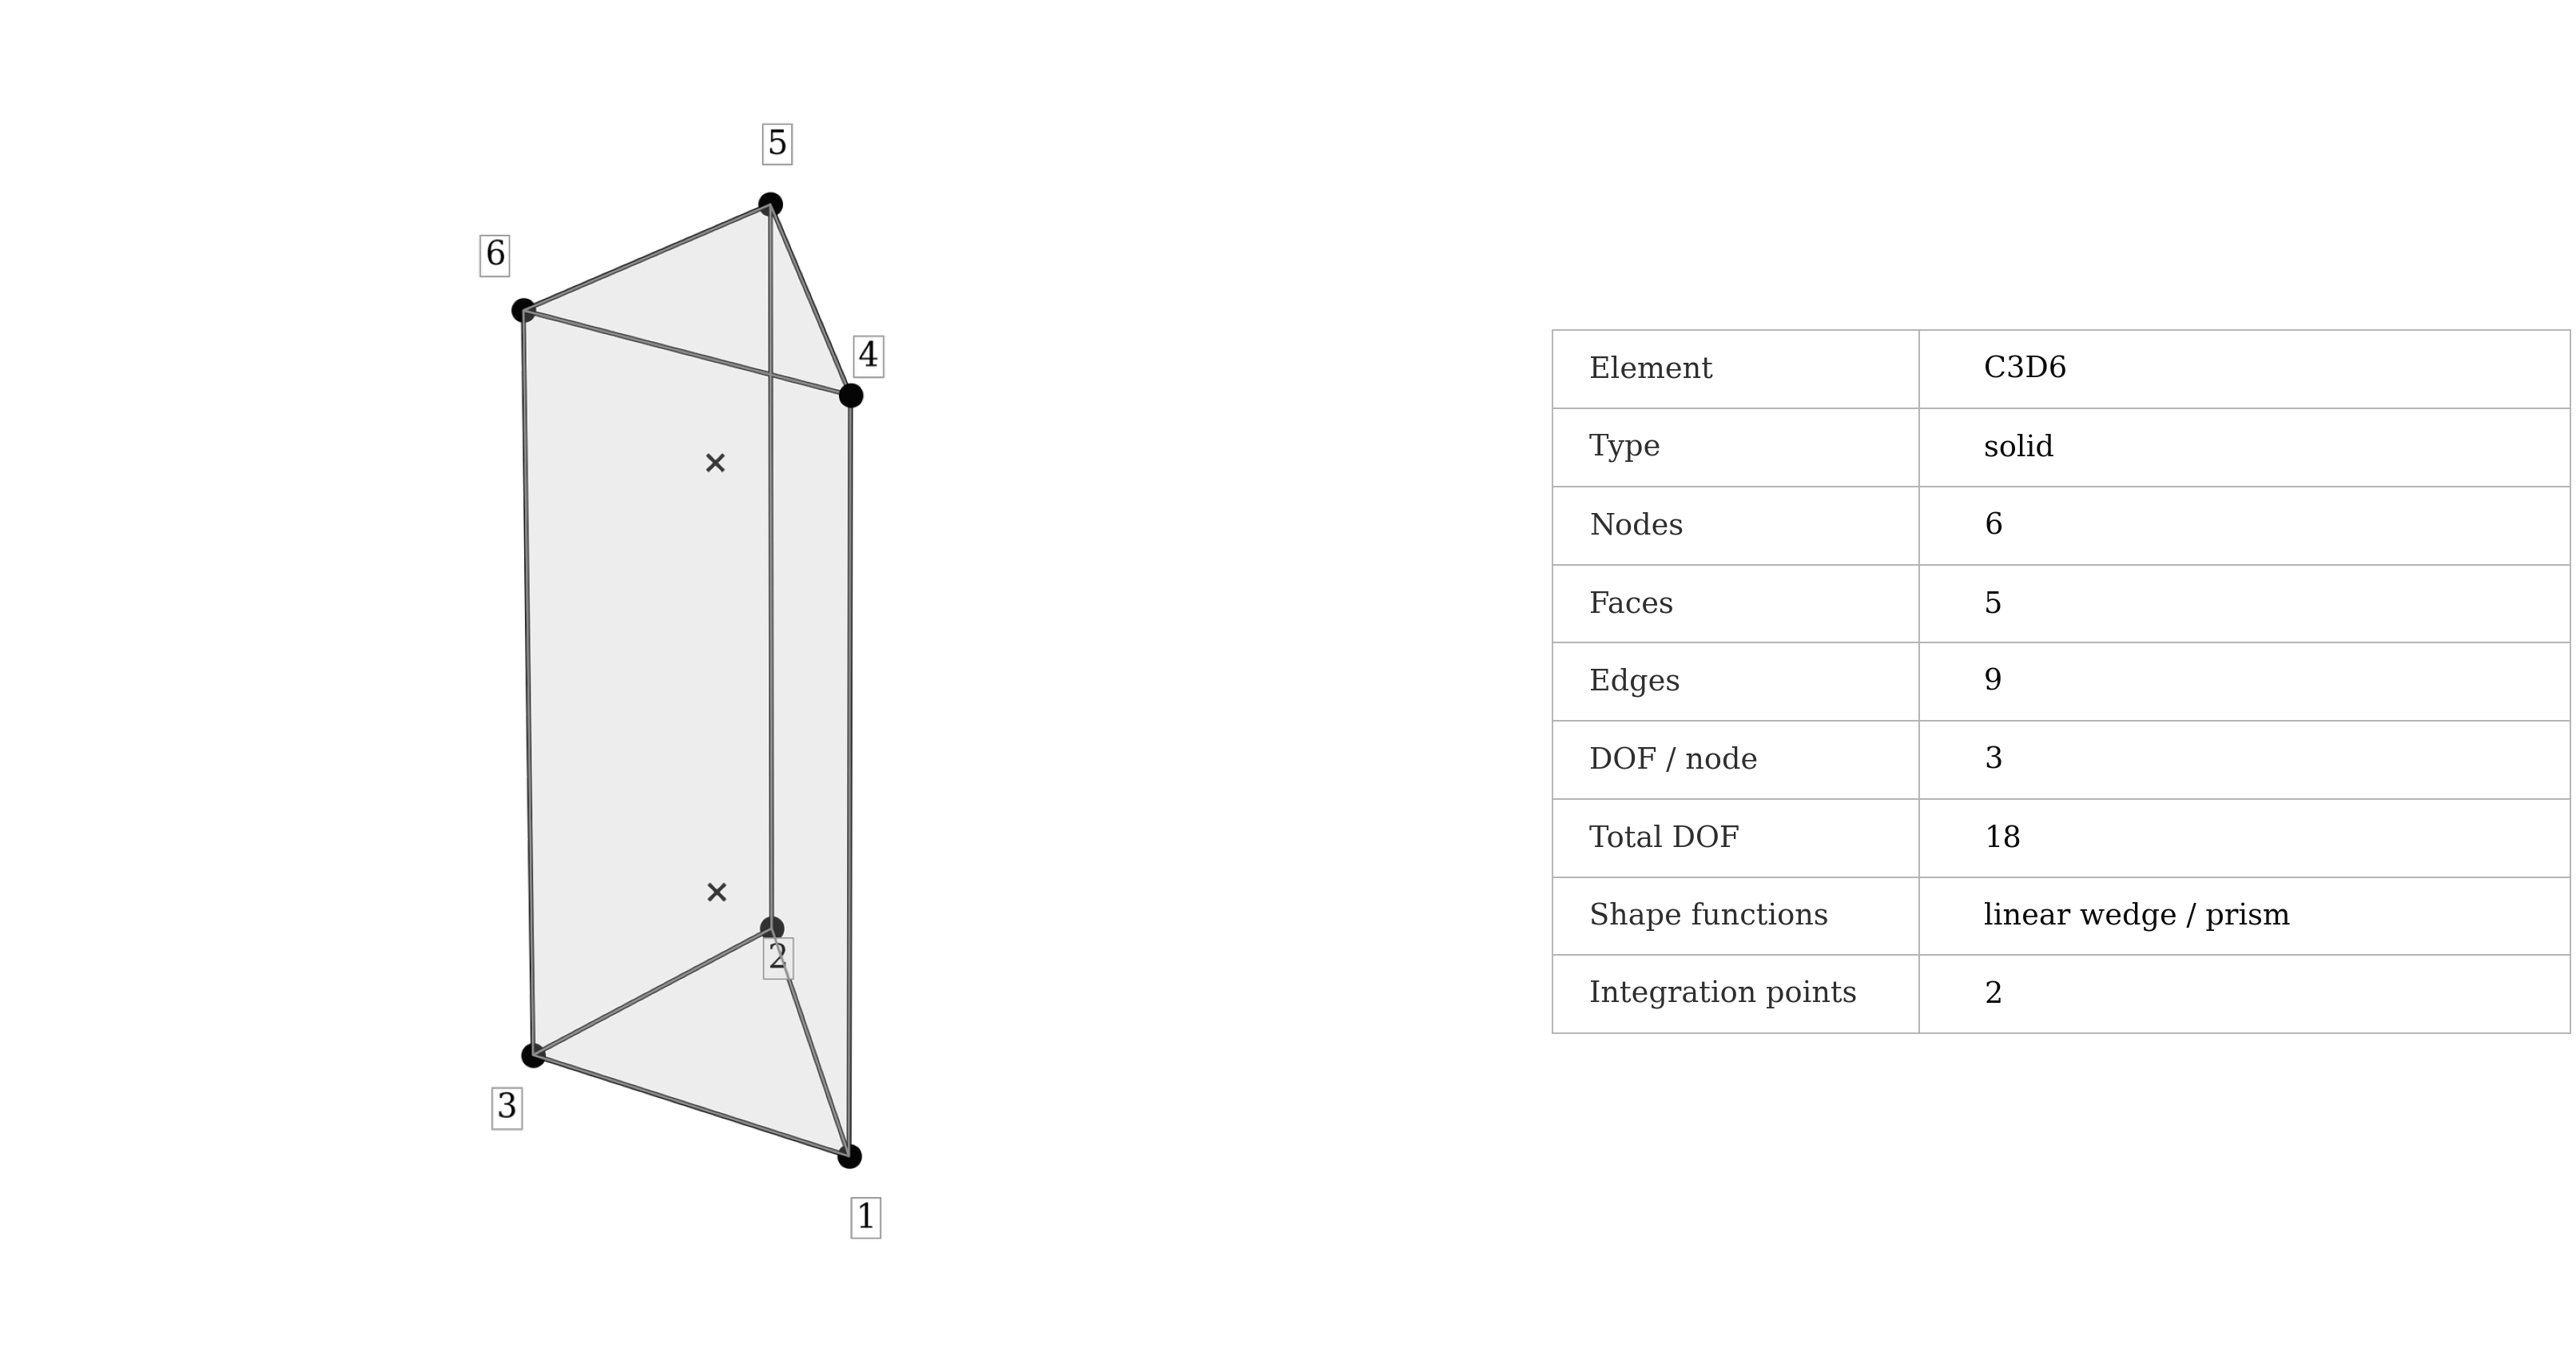
\includegraphics[width=0.78\linewidth]{pages/figures/element_schematics/c3d6_schematic.png}
    \caption{\val{C3D6} wedge element.}
\end{figure}

\begin{syntax}
*ELEMENT, TYPE=C3D6, ELSET=<set>
<id>, <n1>, <n2>, <n3>, <n4>, <n5>, <n6>
\end{syntax}

\val{C3D6} is a linear wedge or prism element. It combines triangular end faces with quadrilateral side faces and is particularly useful for swept meshes, extruded triangular surface meshes, layered regions, and transitions where a purely hexahedral topology is not possible.

A wedge mesh can align naturally with a dominant through-thickness or extrusion direction. This is useful in locally layered solids and prismatic regions because the element rows can follow the physical geometry more consistently than an unstructured tetrahedral mesh.

Like other low-order elements, \val{C3D6} has limited bending and gradient resolution. One or two linear wedges through the thickness of a bending-dominated region are rarely sufficient for accurate stress recovery. Refine in the direction of expected gradients and avoid collapsed triangular faces, excessive twisting between end faces, and highly skewed side faces.

Use \val{C3D6} when wedge topology is geometrically natural. If a quadratic swept mesh is available and higher accuracy is required, \val{C3D15} is the corresponding higher-order choice.

\clearpage
\section{\val{C3D8}: 8-node hexahedral solid}

\begin{figure}[H]
    \centering
    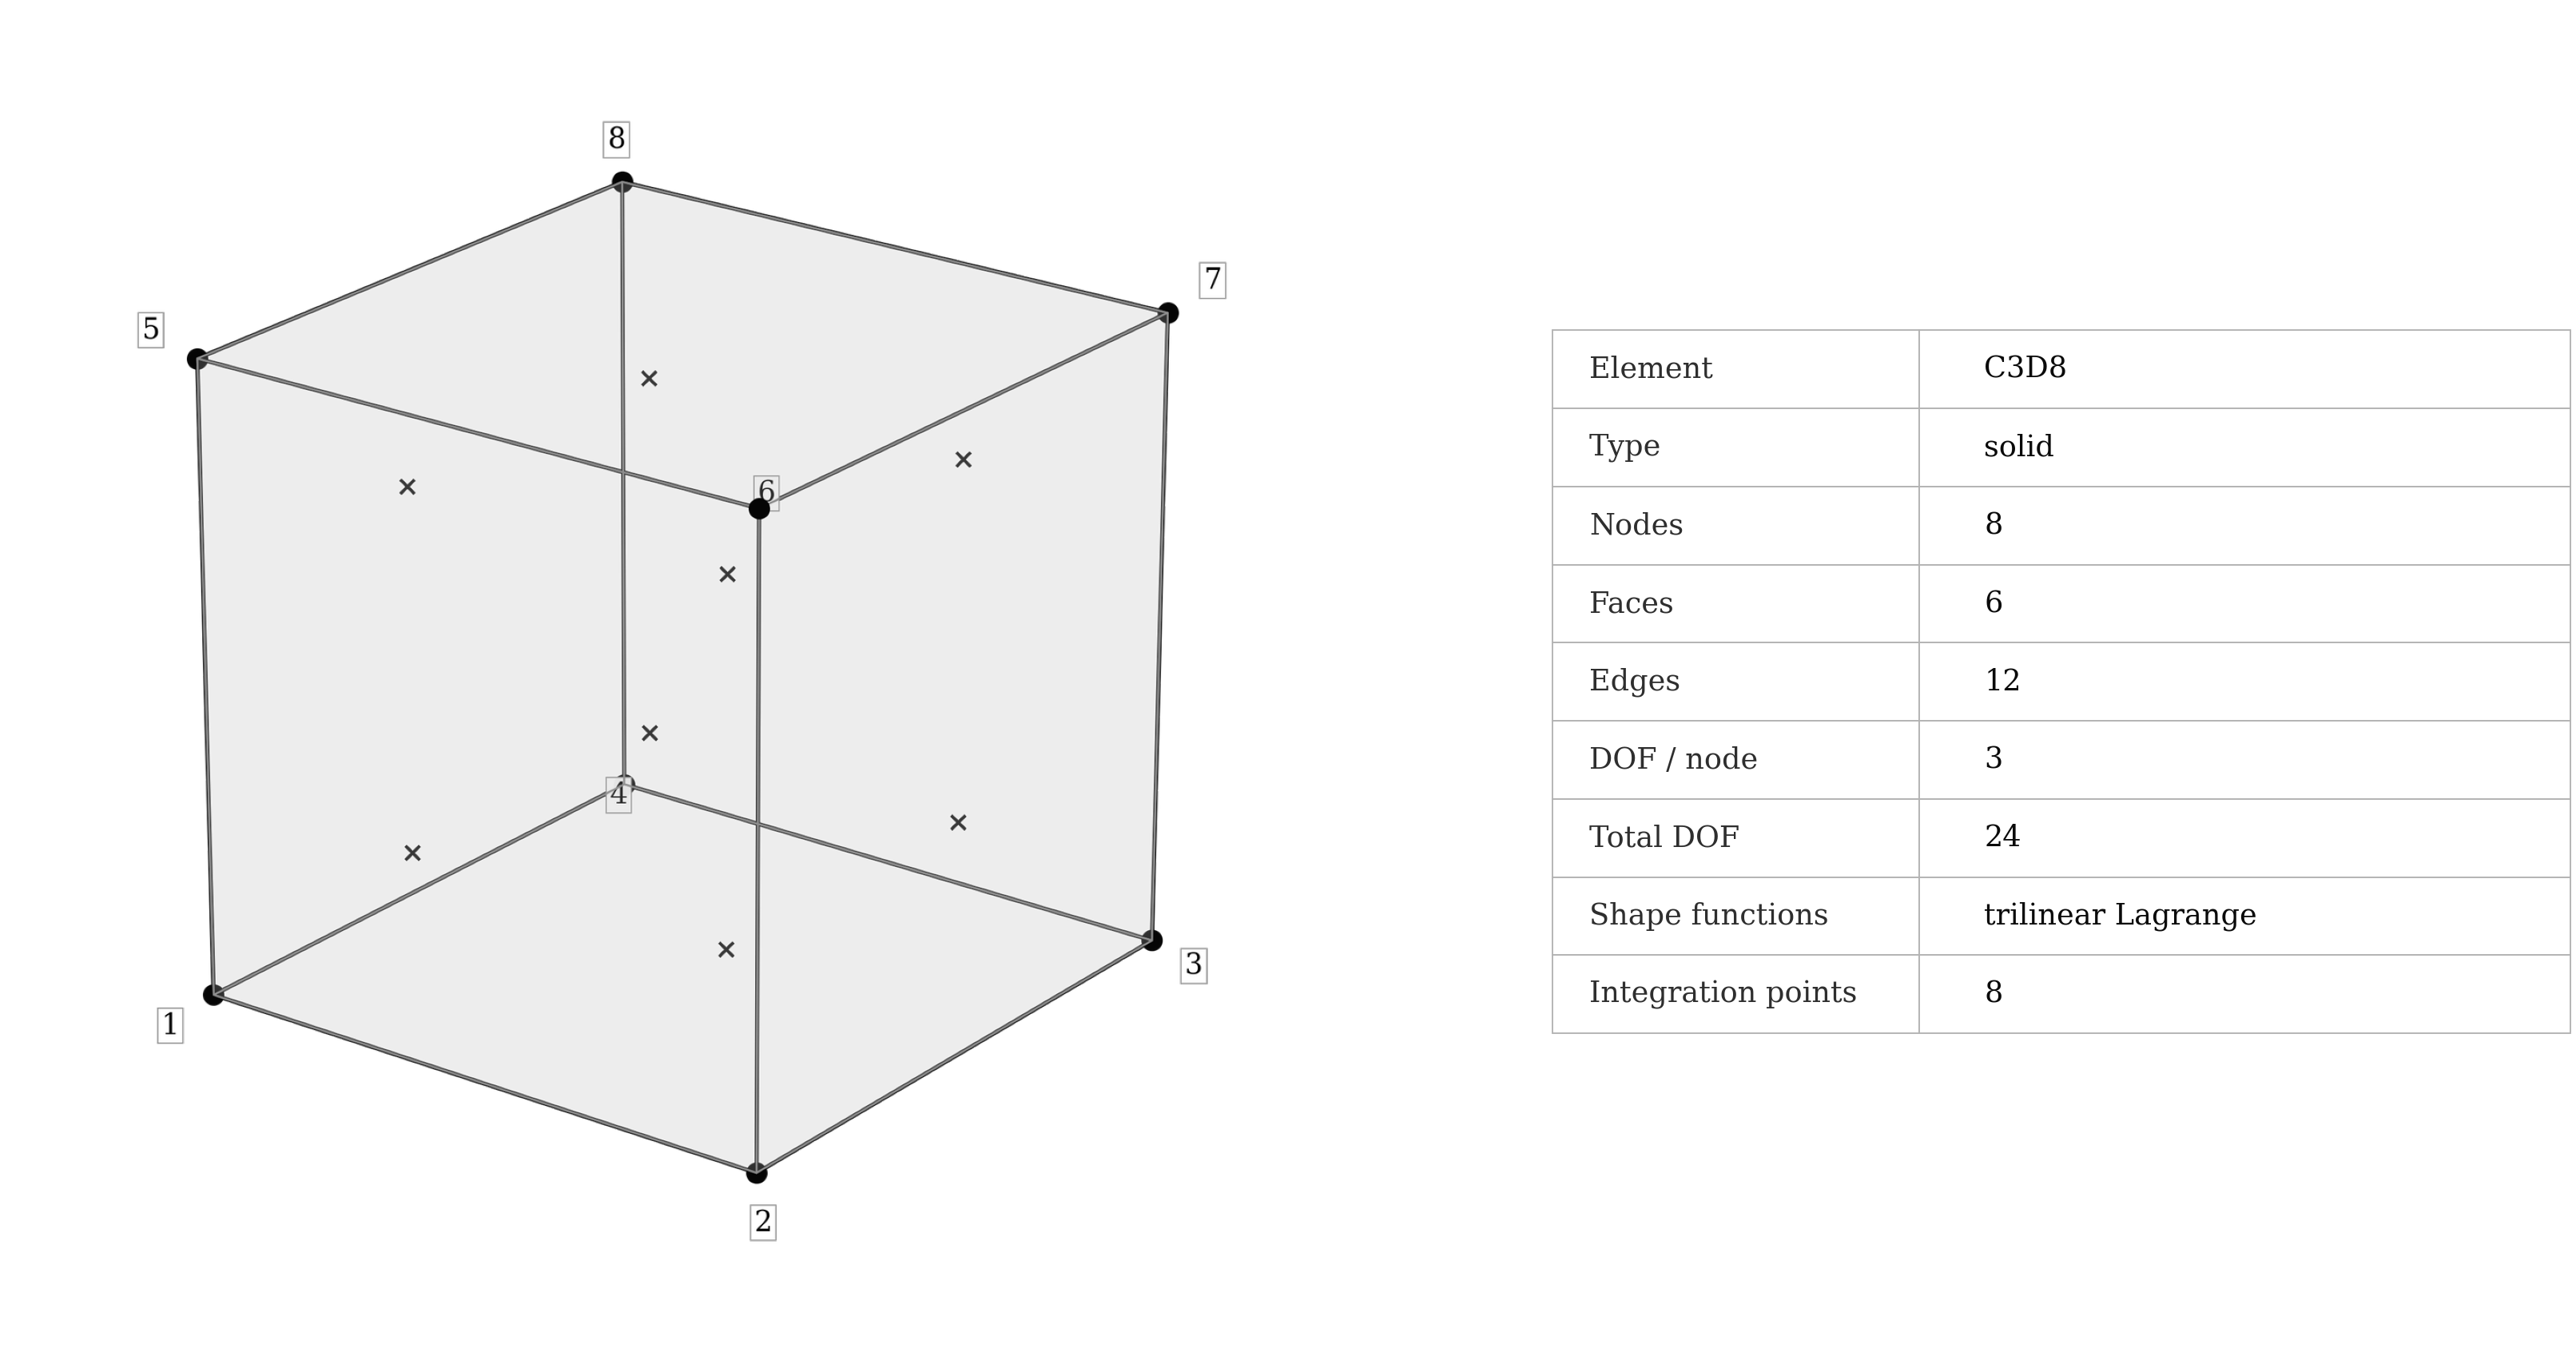
\includegraphics[width=0.82\linewidth]{pages/figures/element_schematics/c3d8_schematic.png}
    \caption{\val{C3D8} hexahedral solid element.}
\end{figure}

\begin{syntax}
*ELEMENT, TYPE=C3D8, ELSET=<set>
<id>, <n1>, <n2>, <n3>, <n4>, <n5>, <n6>, <n7>, <n8>
\end{syntax}

\val{C3D8} is the standard low-order hexahedral continuum element. It uses trilinear displacement interpolation and full integration. For regular block-like, swept, or layered meshes it is often an efficient general-purpose solid because element directions can follow geometry and material orientation naturally.

Hexahedral topology makes it easy to control the number of elements through thickness and along structural load paths. A good \val{C3D8} mesh is therefore attractive for plates modelled with solids, bonded layers, spars, ribs, extruded components, and regions where orthotropic material axes should follow the mesh.

The element remains low order. A coarse mesh can be too stiff in bending, and straight element edges only approximate curved boundaries. Use several elements through thickness when solid bending stresses are important and refine curved or stress-critical geometry sufficiently.

Warping, skew, negative Jacobians, and extreme aspect ratios can destroy the advantages of the hexahedral topology. A clean quadratic tetrahedral mesh can be better than a badly distorted hexahedral mesh. Inspect mesh quality instead of selecting \val{C3D8} solely because hexahedra are usually preferred.

\clearpage
\section{\val{C3D8R}: reduced-integration 8-node hexahedral solid}

\begin{figure}[H]
    \centering
    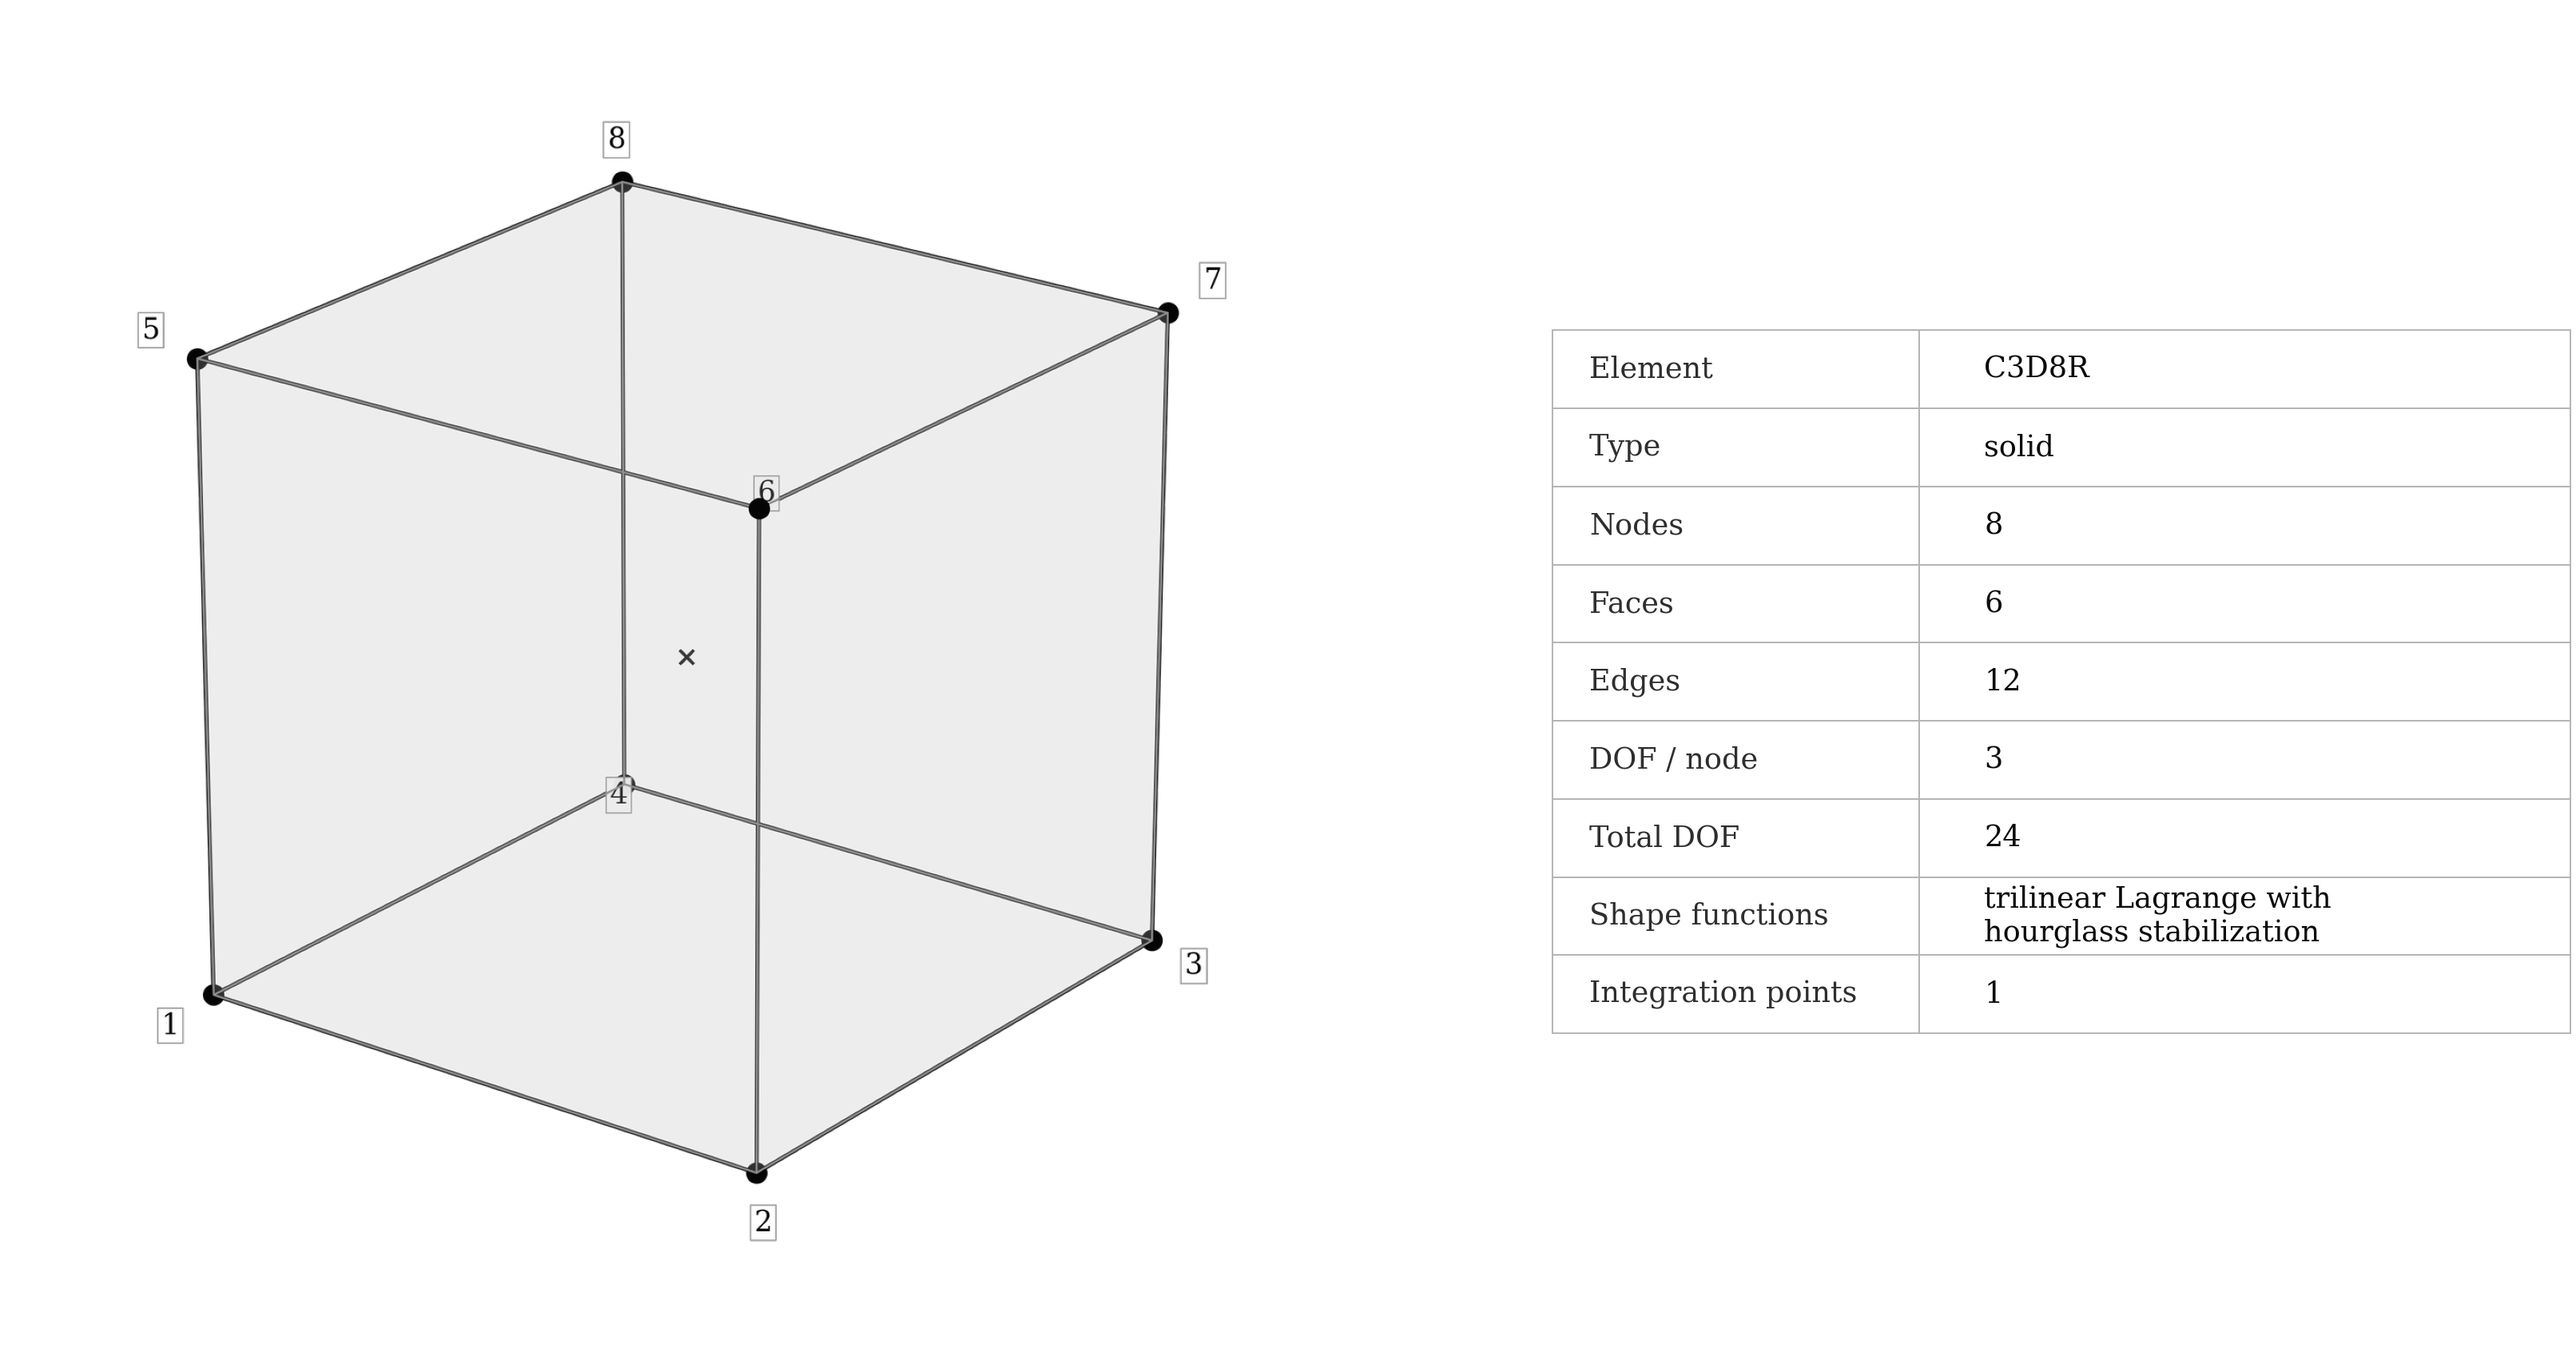
\includegraphics[width=0.82\linewidth]{pages/figures/element_schematics/c3d8r_schematic.png}
    \caption{\val{C3D8R} reduced-integration hexahedral solid element.}
\end{figure}

\begin{syntax}
*ELEMENT, TYPE=C3D8R, ELSET=<set>
<id>, <n1>, <n2>, <n3>, <n4>, <n5>, <n6>, <n7>, <n8>
\end{syntax}

\val{C3D8R} uses the same eight-node topology as \val{C3D8} but evaluates the continuum contribution with one integration point at the element centre. Reduced integration lowers assembly cost and avoids some of the excessive stiffness that a fully integrated low-order hexahedron can exhibit in bending-dominated states.

One-point integration also introduces zero-energy hourglass deformation modes. FEMaster therefore adds hourglass stabilization. The primitive scalar hourglass patterns are based on the four non-affine modes
\[
\gamma_1=s\,t,\qquad
\gamma_2=t\,r,\qquad
\gamma_3=r\,s,\qquad
\gamma_4=r\,s\,t.
\]
These modes are projected so that affine displacement fields are not penalized. The stabilization scale is based on the element reference volume, the reference geometry gradients, and an effective shear stiffness derived from the constitutive tangent.

The practical consequence is that \val{C3D8R} should be judged not only by Newton convergence but also by its deformation pattern and stabilization sensitivity. A model may converge while still exhibiting nonphysical hourglass deformation if the mesh is too coarse or badly distorted. Compare suspicious regions with \val{C3D8}, refine the mesh, and inspect whether the response changes strongly when the hourglass-sensitive deformation is resolved geometrically.

For severe finite rotations or highly distorted elements, reduced-integration stabilization deserves particular scrutiny. Use \val{C3D8R} deliberately when its lower locking tendency or cost is beneficial, rather than as an automatic replacement for \val{C3D8}.

\clearpage
\section{\val{C3D10}: 10-node quadratic tetrahedral solid}

\begin{figure}[H]
    \centering
    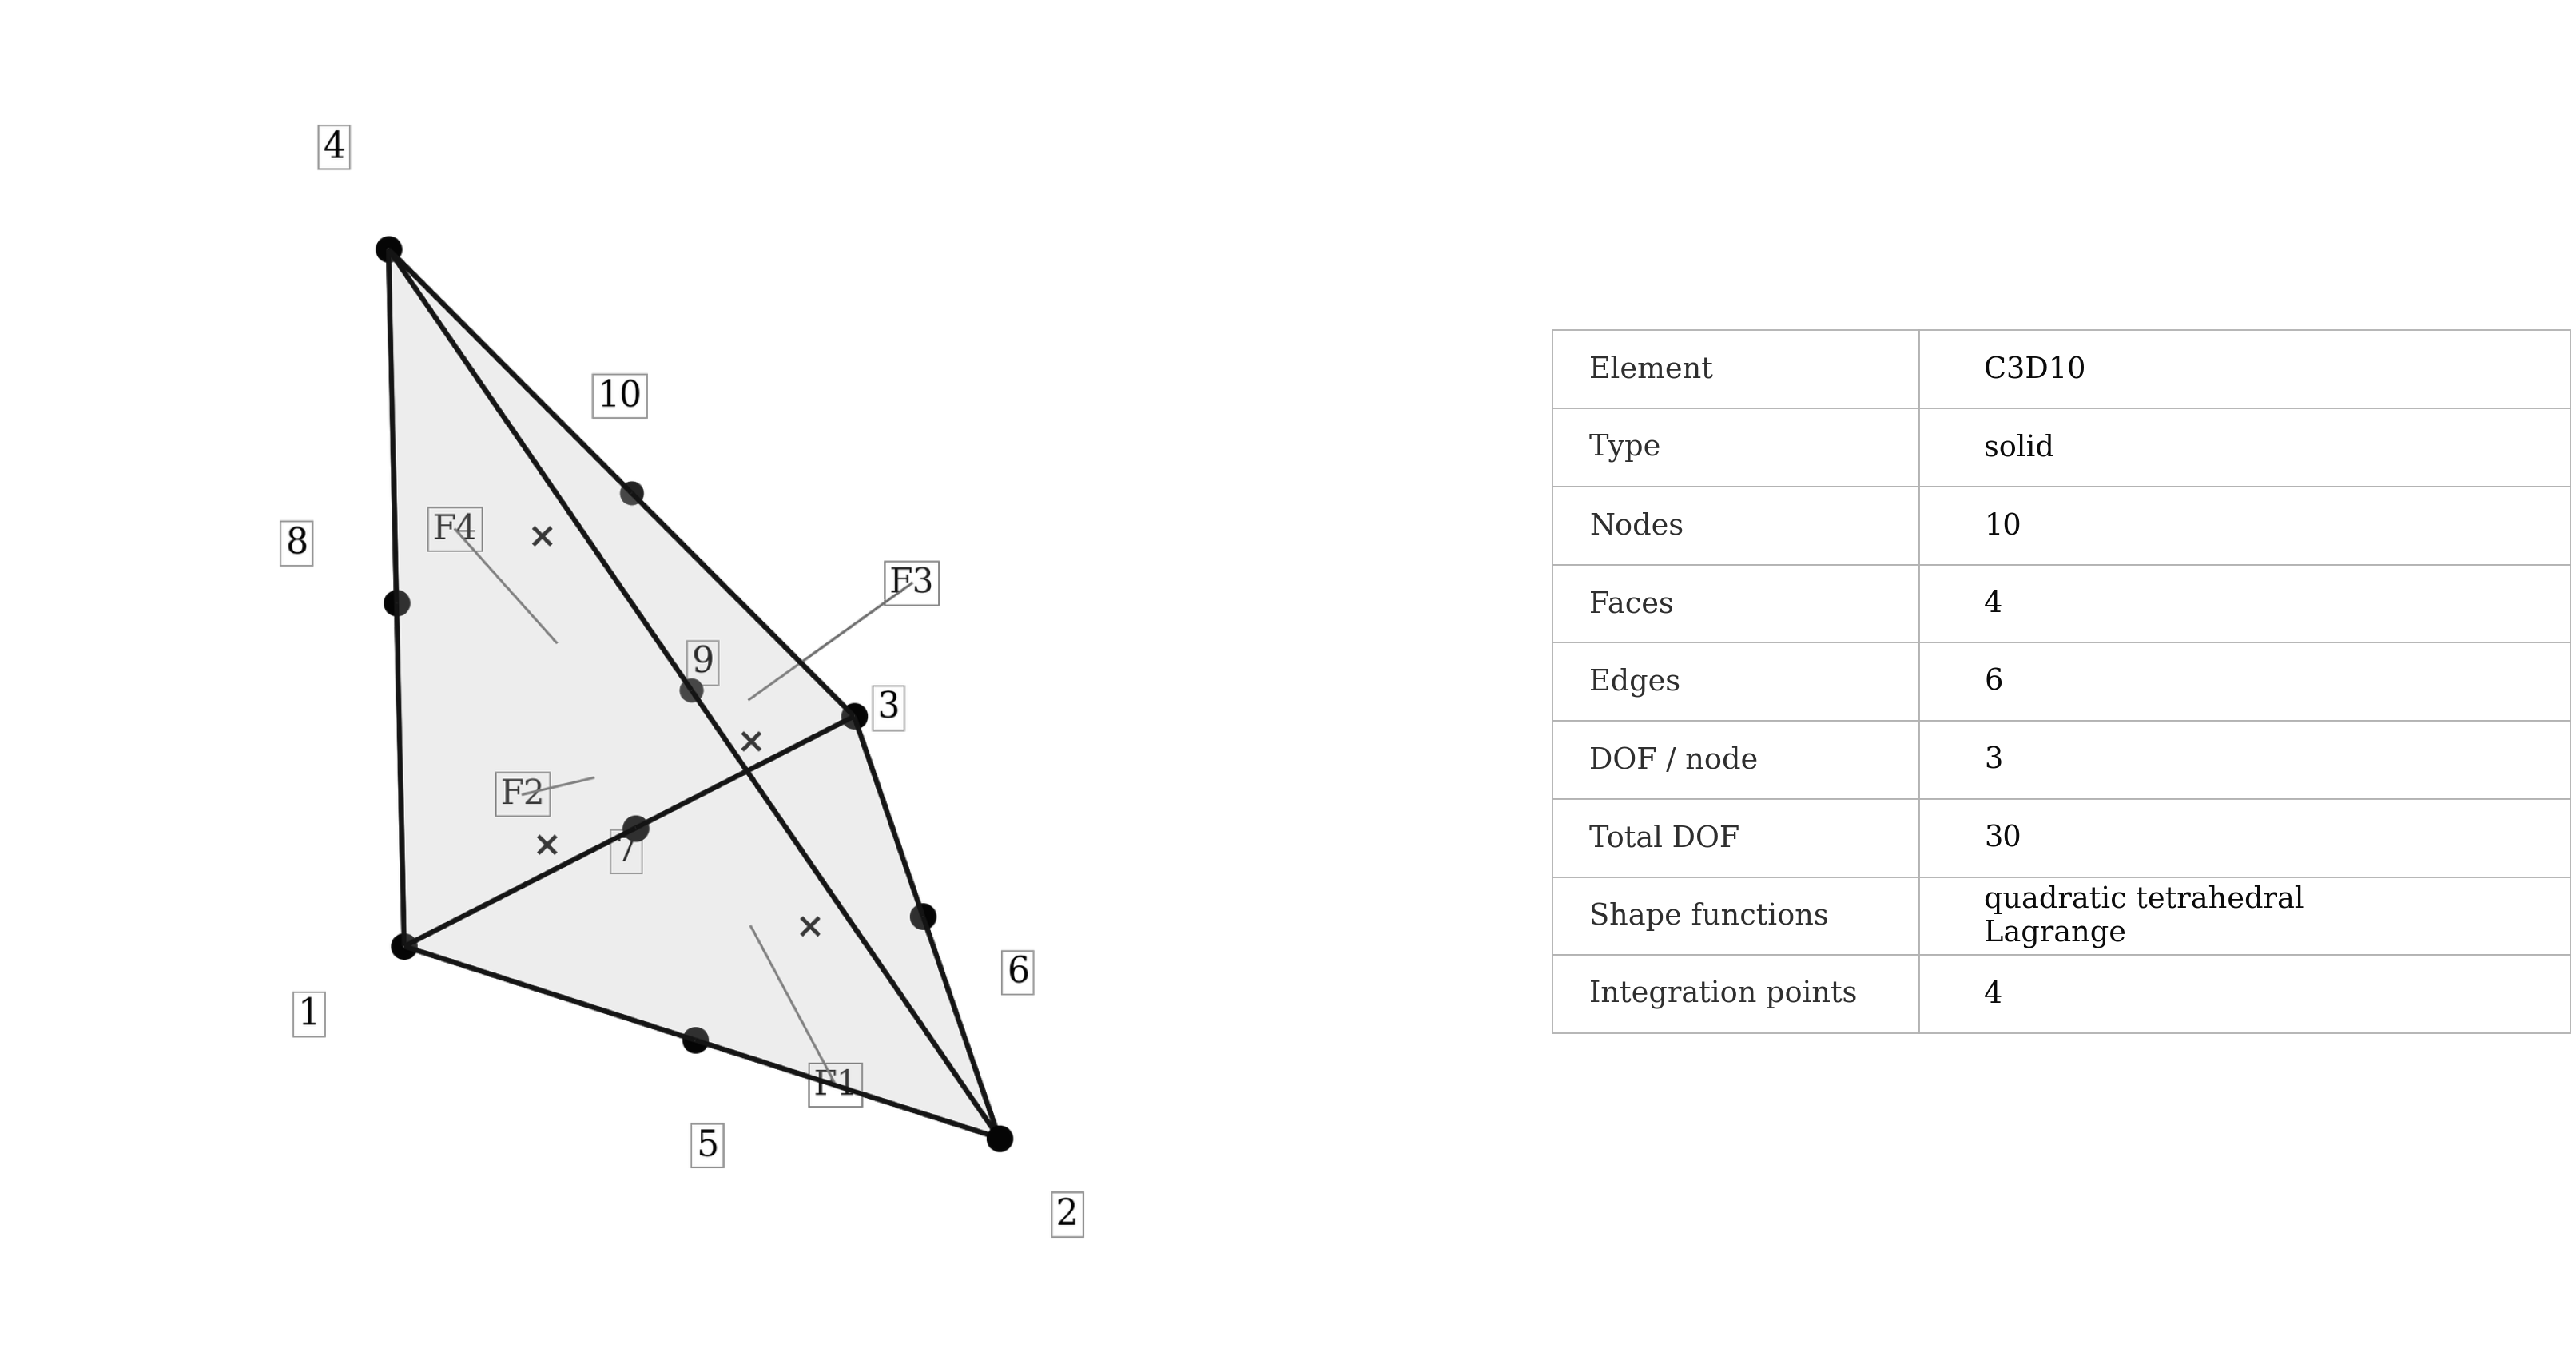
\includegraphics[width=0.80\linewidth]{pages/figures/element_schematics/c3d10_schematic.png}
    \caption{\val{C3D10} quadratic tetrahedral element.}
\end{figure}

\begin{syntax}
*ELEMENT, TYPE=C3D10, ELSET=<set>
<id>, <n1>, <n2>, <n3>, <n4>, <n5>, <n6>, <n7>, <n8>, <n9>, <n10>
\end{syntax}

\val{C3D10} is the quadratic tetrahedral solid. Six midside nodes augment the four corner nodes and allow quadratic displacement interpolation. Compared with \val{C3D4}, the element can represent curved deformation, bending, and stress gradients far more efficiently.

For automatic tetrahedral meshing, \val{C3D10} is generally the preferred engineering stress element. It keeps the geometric flexibility of tetrahedra while reducing the excessive stiffness and piecewise-constant strain behaviour associated with linear tetrahedra.

The quadratic geometry mapping also represents curved boundaries more accurately when midside nodes follow the CAD geometry. Those midside positions must remain sensible: badly displaced midside nodes can create a distorted mapping even if the corner tetrahedron appears acceptable.

The element costs more per cell than \val{C3D4}, but substantially fewer cells may be required for comparable displacement and stress accuracy. Refinement is still required near singularities, sharp re-entrant corners, and concentrated loads where no polynomial element can make a mathematical singularity disappear.

\clearpage
\section{\val{C3D15}: 15-node quadratic wedge solid}

\begin{figure}[H]
    \centering
    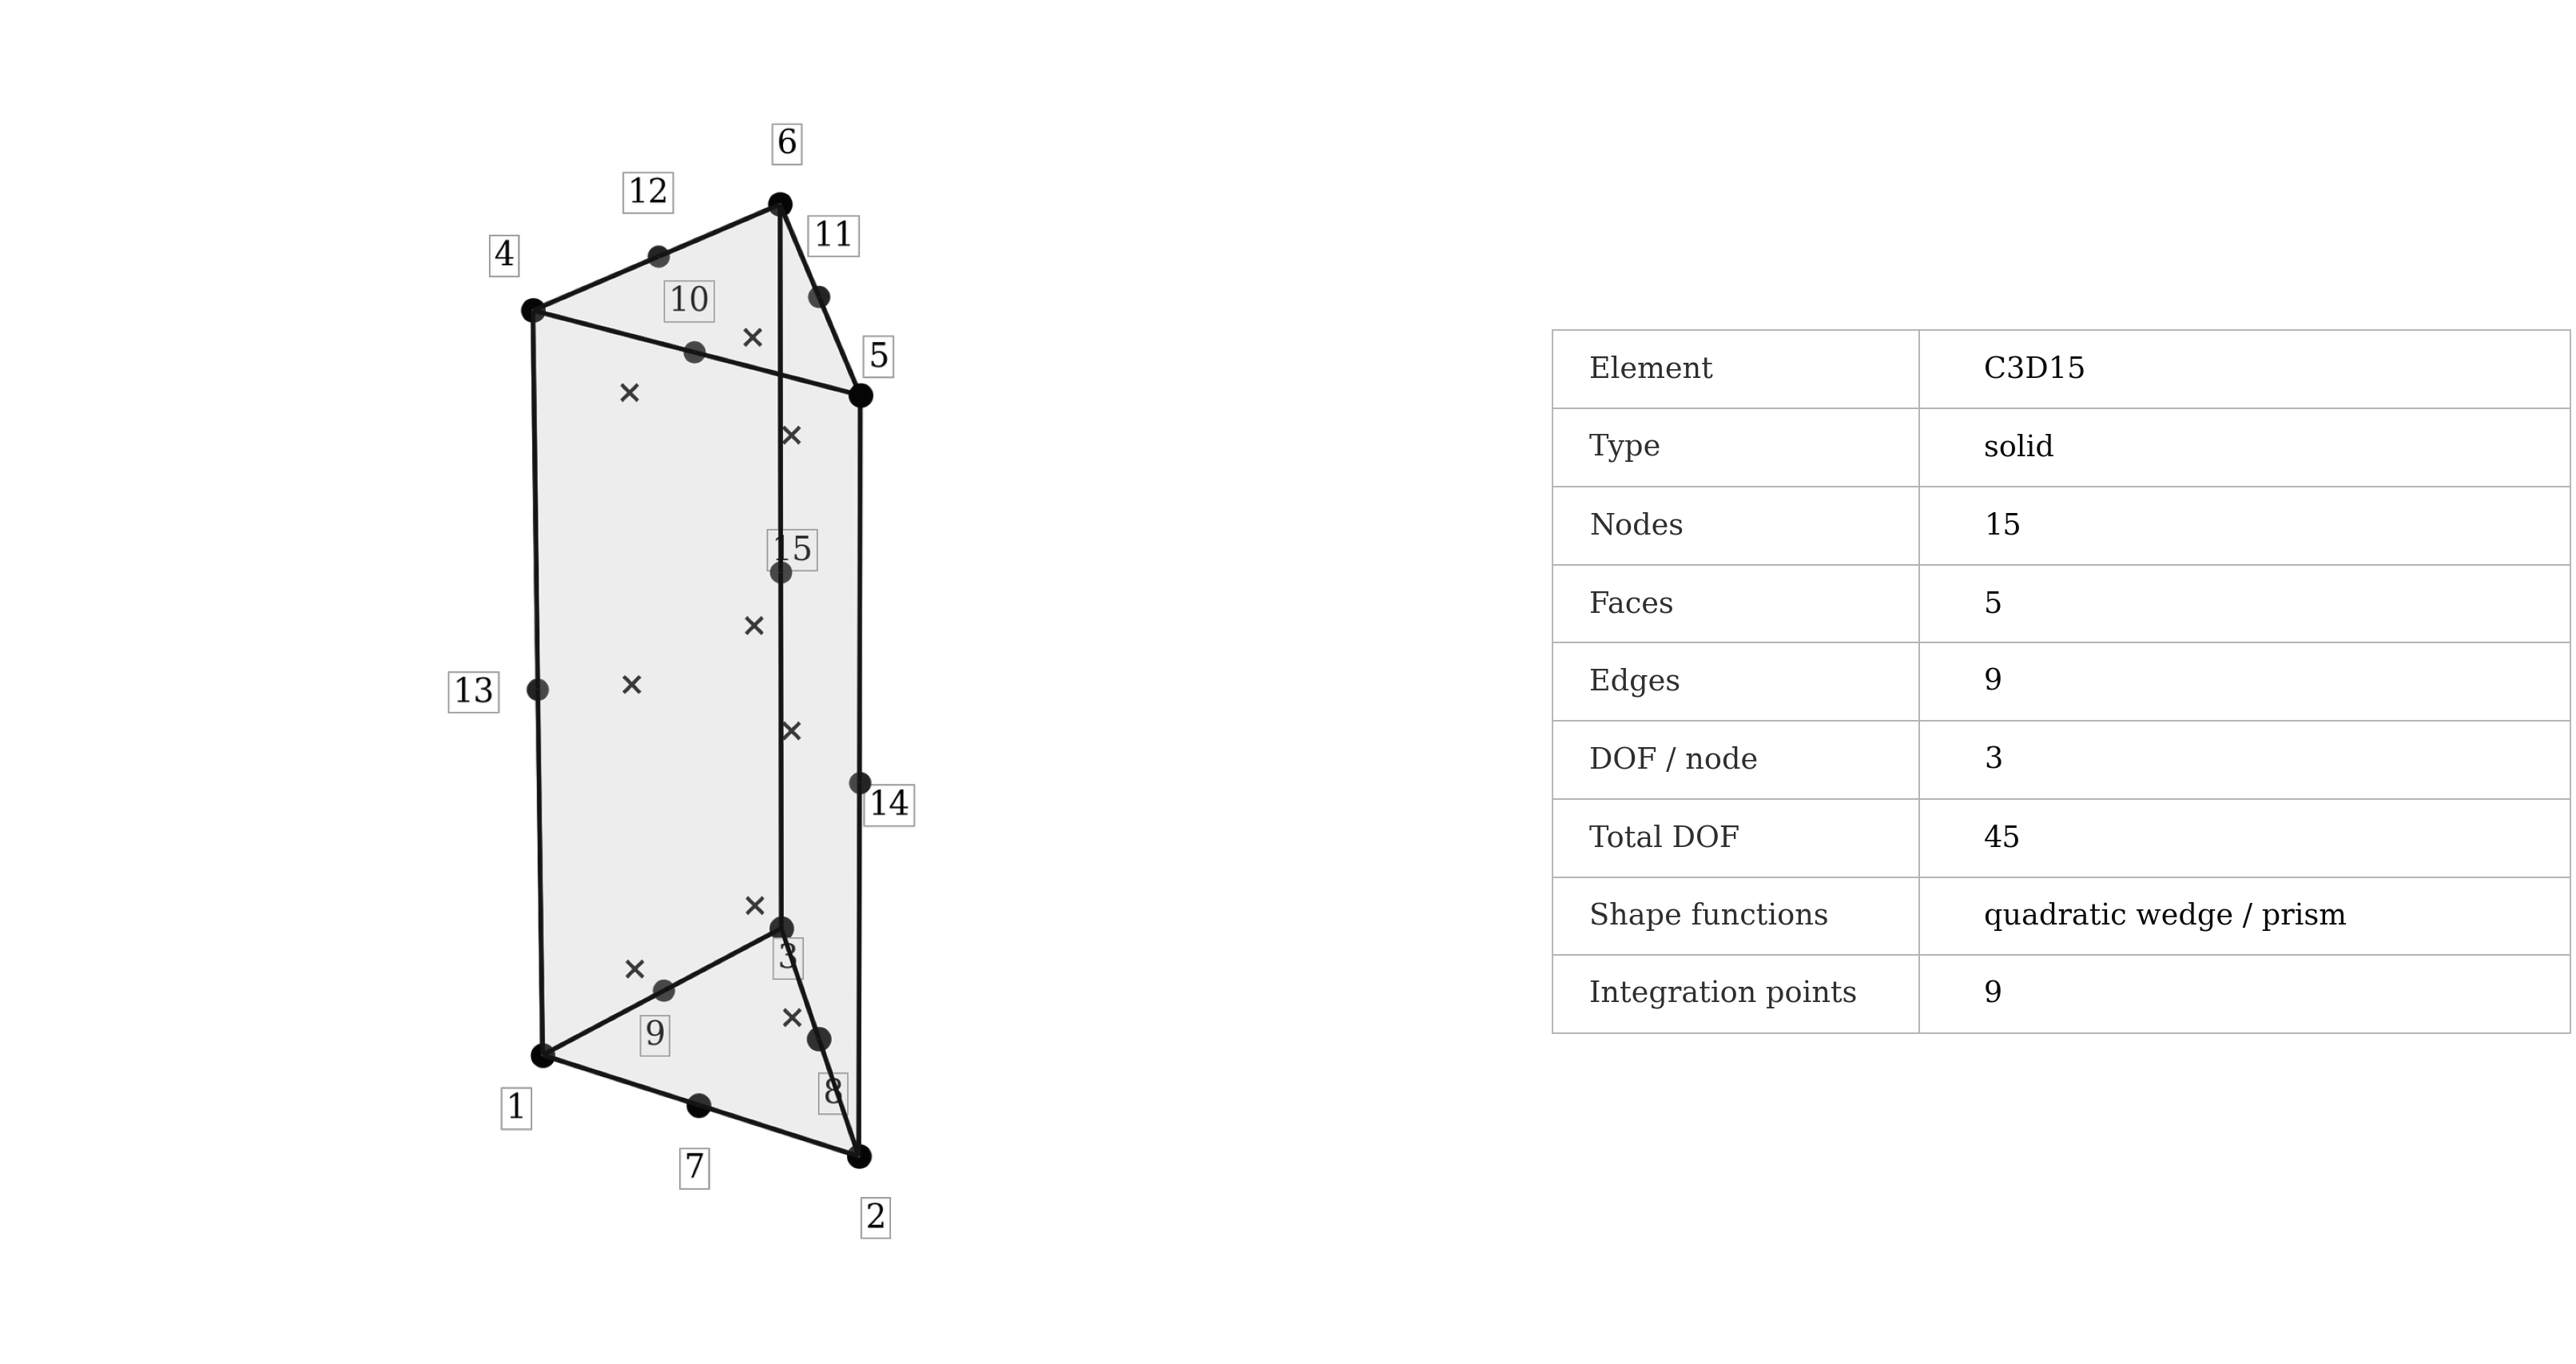
\includegraphics[width=0.80\linewidth]{pages/figures/element_schematics/c3d15_schematic.png}
    \caption{\val{C3D15} quadratic wedge element.}
\end{figure}

\begin{syntax}
*ELEMENT, TYPE=C3D15, ELSET=<set>
<id>, <n1>, ..., <n15>
\end{syntax}

\val{C3D15} is the quadratic counterpart of the six-node wedge. It adds midside nodes and can represent curvature, bending, and through-thickness gradients more effectively than \val{C3D6}. It is particularly useful in higher-order swept meshes and in prismatic regions created by extruding a quadratic triangular surface mesh.

The element is attractive when wedge topology is natural but low-order through-thickness behaviour is insufficient. Curved swept solids, local layered regions, and transition zones can often be represented with fewer elements than would be needed with \val{C3D6}.

Higher-order mapping increases sensitivity to midside-node placement. The triangular end faces should remain well shaped, the side faces should not twist excessively, and midside nodes should follow the intended geometry smoothly. A high-order wedge with a poor mapping is not automatically more accurate than a clean low-order mesh.

Use \val{C3D15} for deliberate quadratic wedge meshes. If the geometry supports a structured quadratic hexahedral mesh, \val{C3D20} may provide a more regular discretization; for fully unstructured complex geometry, \val{C3D10} is often easier to generate robustly.

\clearpage
\section{\val{C3D20}: 20-node quadratic hexahedral solid}

\begin{figure}[H]
    \centering
    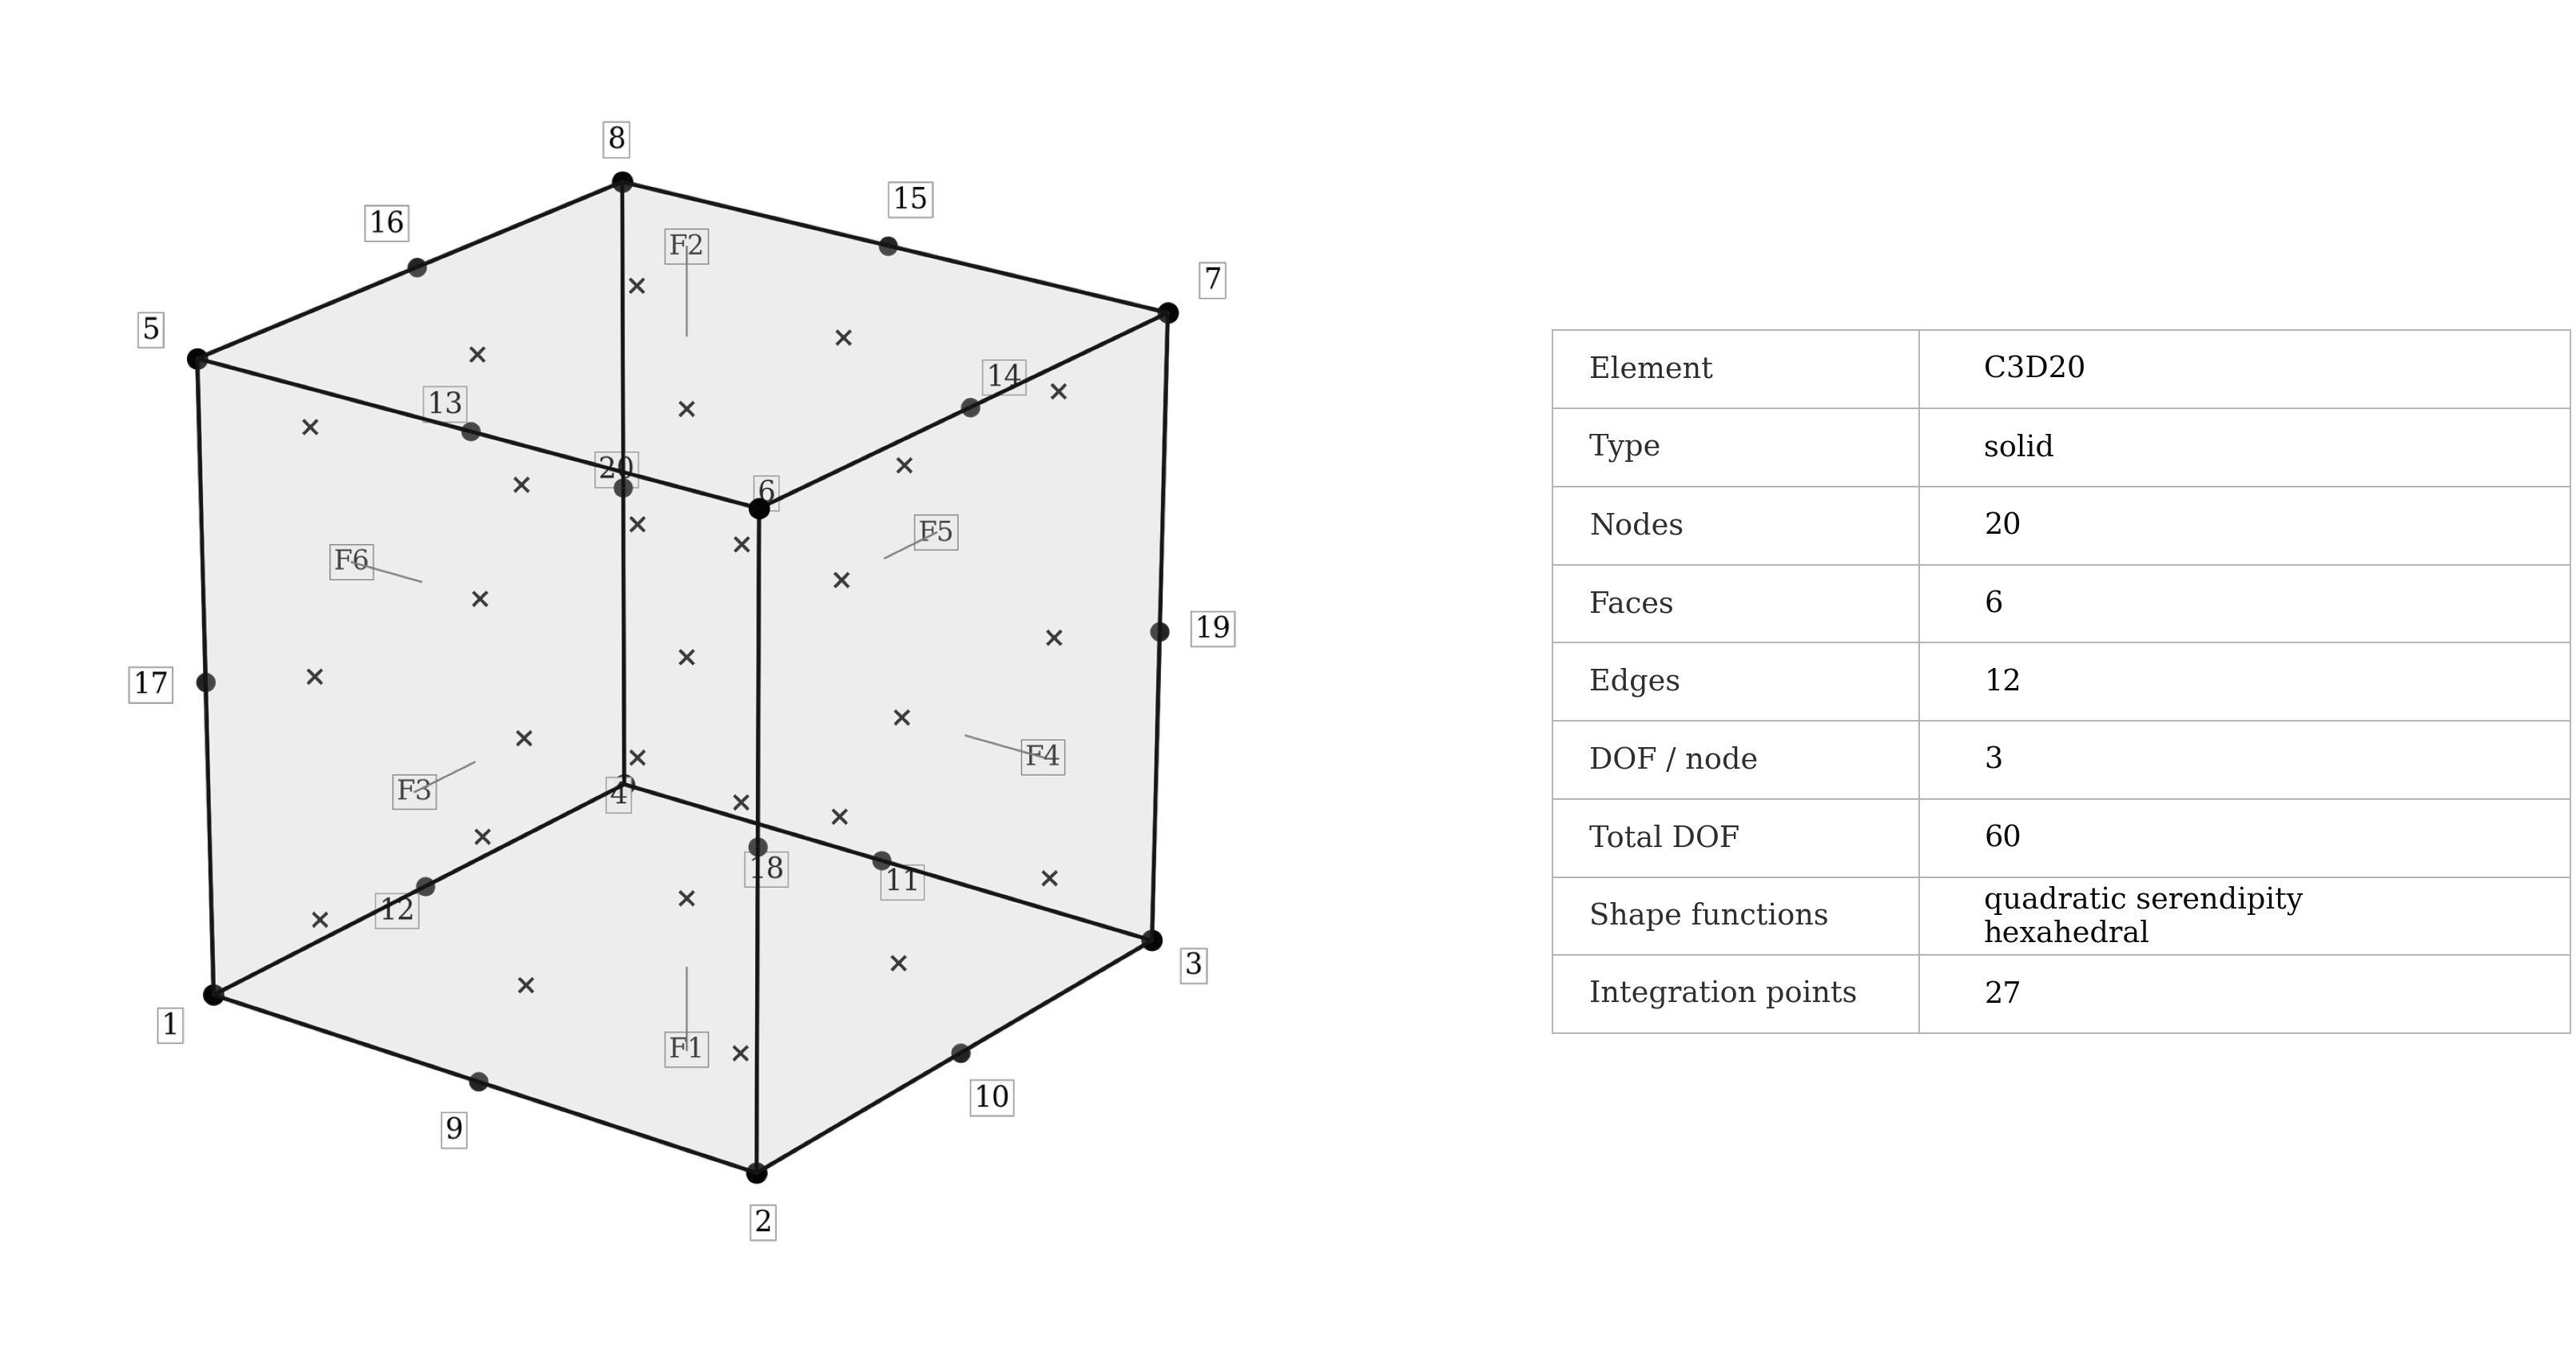
\includegraphics[width=0.82\linewidth]{pages/figures/element_schematics/c3d20_schematic.png}
    \caption{\val{C3D20} quadratic hexahedral element.}
\end{figure}

\begin{syntax}
*ELEMENT, TYPE=C3D20, ELSET=<set>
<id>, <n1>, ..., <n20>
\end{syntax}

\val{C3D20} is the full-integration quadratic hexahedral solid. The eight corner nodes are supplemented by twelve midside nodes, giving the element substantially better bending and stress-gradient representation than \val{C3D8}. Curved geometry can also be represented more accurately when midside nodes follow the physical boundary.

For smooth structural fields and high-quality structured meshes, \val{C3D20} is one of the most accurate solid choices available in FEMaster. It is well suited to curved blocks, swept volumes, thick structural regions, and stress-recovery problems where a high-order hexahedral mesh can be generated reliably.

The main costs are larger element matrices and stricter geometric quality requirements. Distortion of a quadratic mapping can be more harmful than distortion of a linear one because the midside nodes participate directly in the geometry interpolation. Check Jacobian quality and avoid arbitrary movement of midside nodes.

Choose \val{C3D20} when accuracy and mesh quality justify the additional cost. For models dominated by linear global stiffness where a fine regular mesh already exists, \val{C3D8} may remain more economical.

\clearpage
\section{\val{C3D20R}: 20-node reduced-integration hexahedral solid}

\begin{figure}[H]
    \centering
    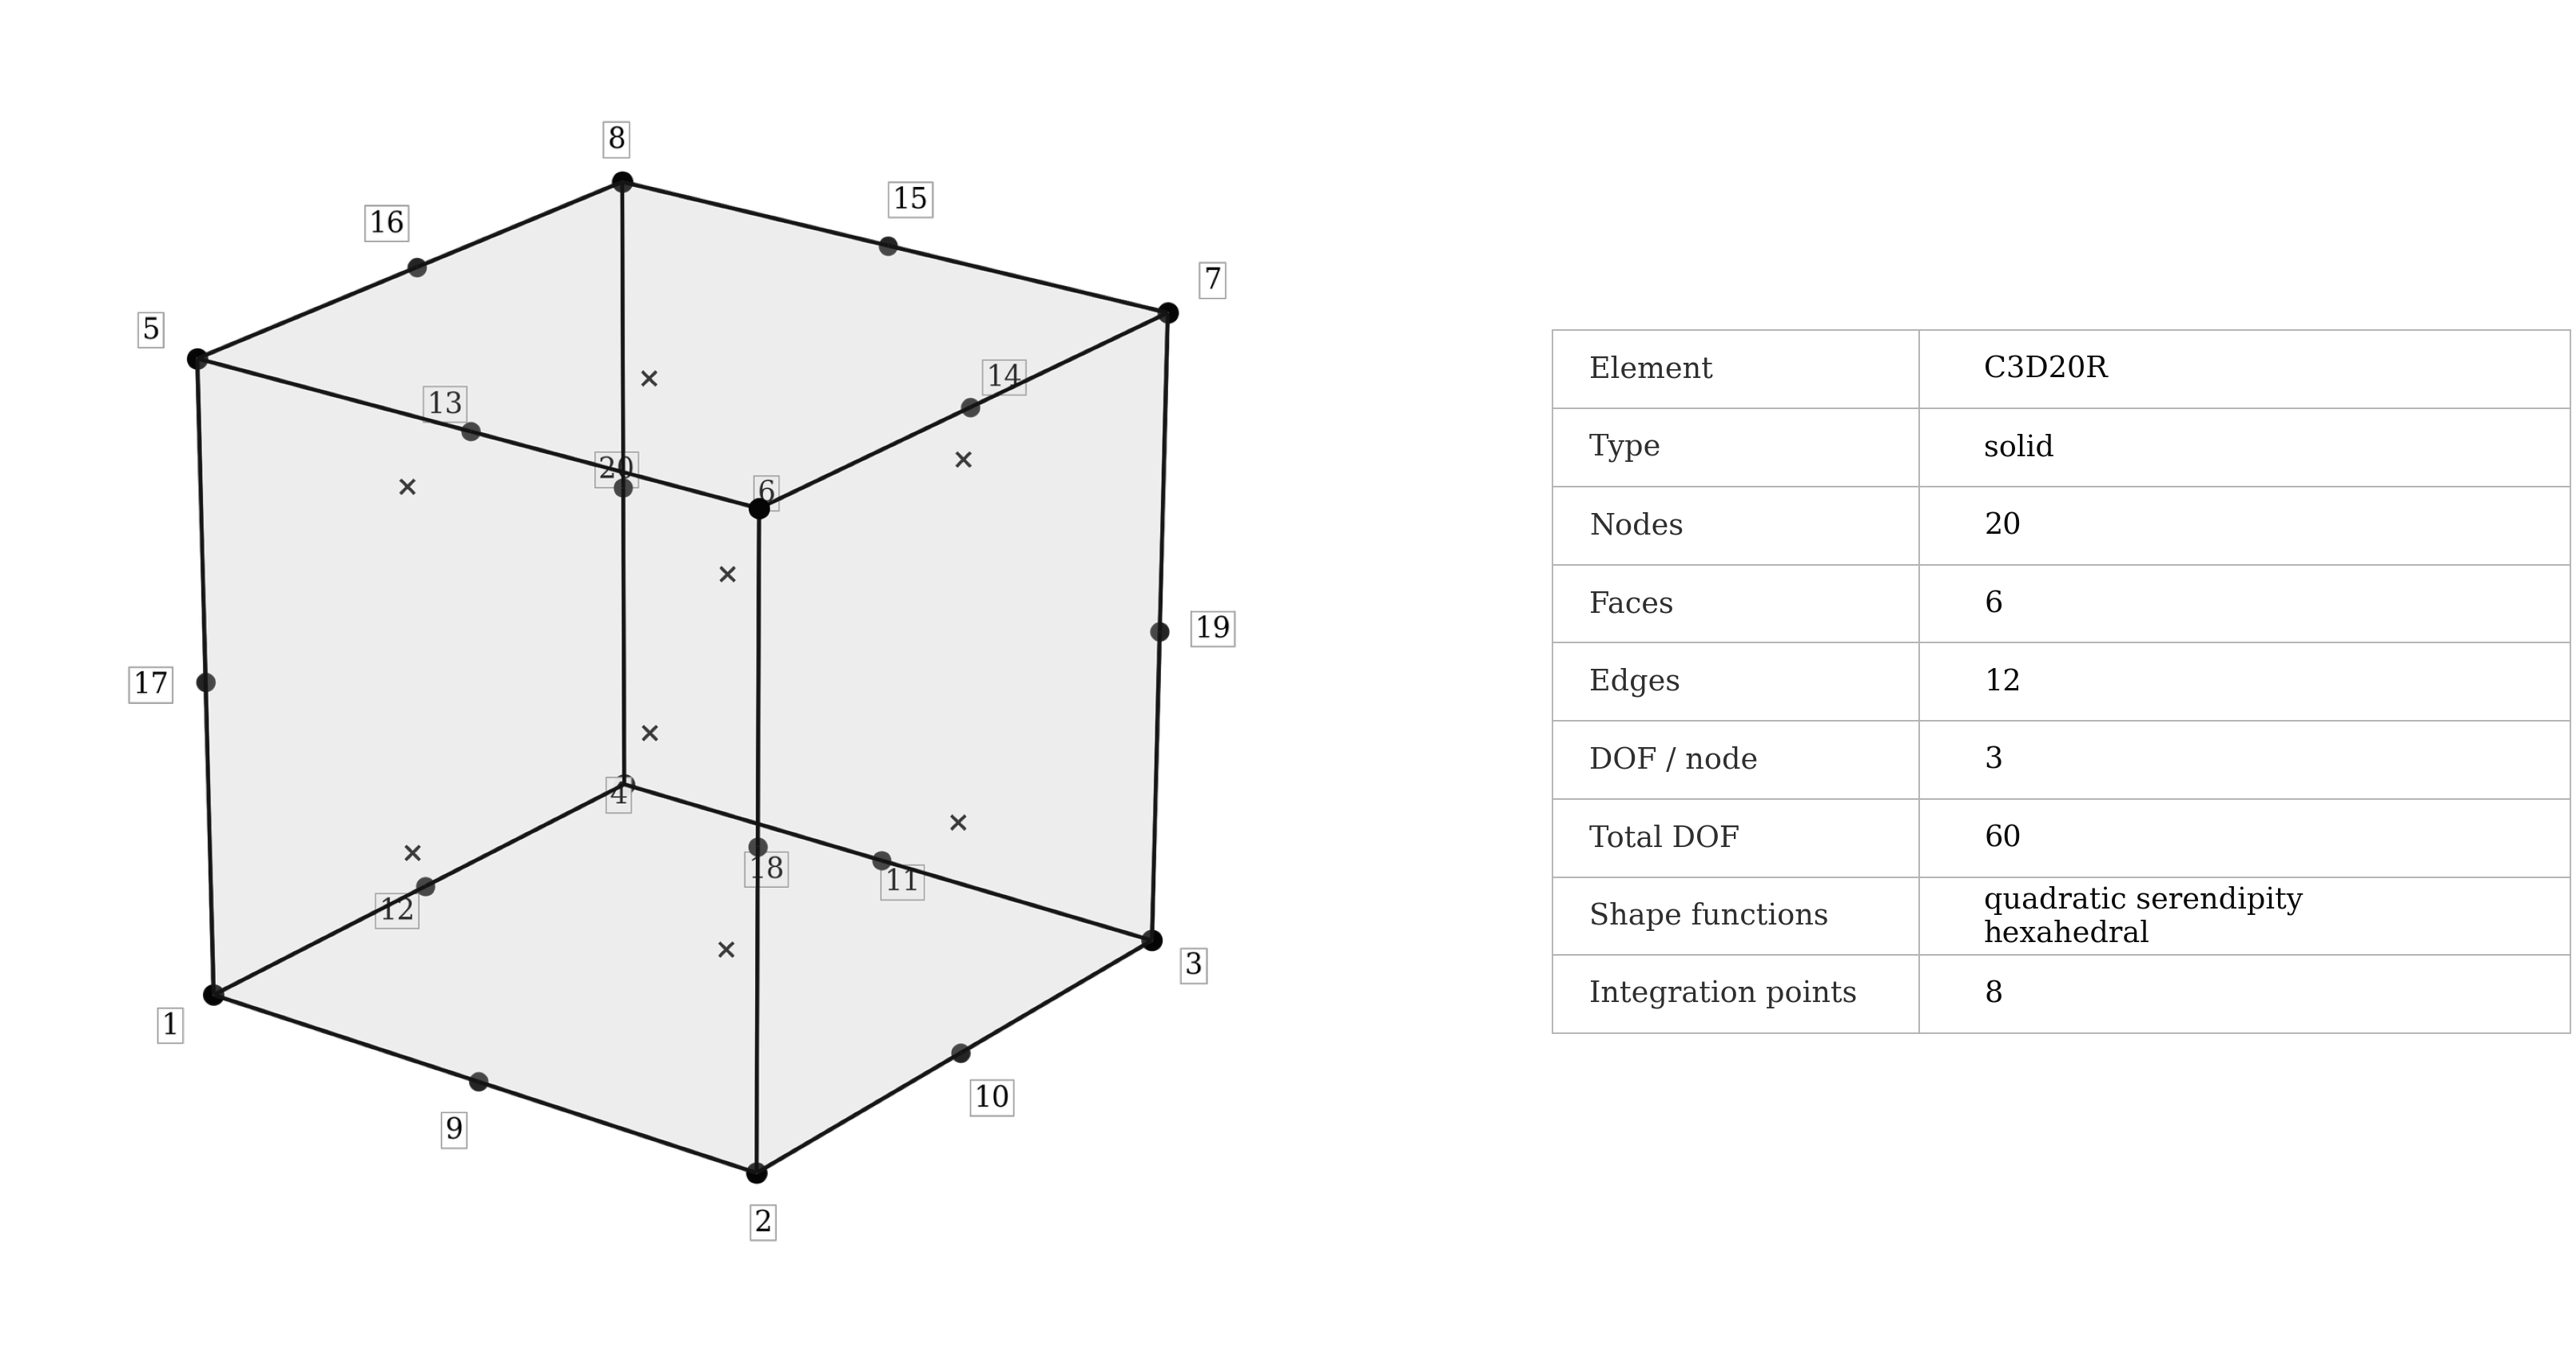
\includegraphics[width=0.82\linewidth]{pages/figures/element_schematics/c3d20r_schematic.png}
    \caption{\val{C3D20R} reduced-integration quadratic hexahedral element.}
\end{figure}

\begin{syntax}
*ELEMENT, TYPE=C3D20R, ELSET=<set>
<id>, <n1>, ..., <n20>
\end{syntax}

\val{C3D20R} uses the same twenty-node topology and quadratic interpolation as \val{C3D20}, but the stiffness contribution is evaluated with reduced integration. The reduced rule lowers cost and can improve behaviour in states where full integration introduces excessive constraint or stiffness.

Reduced integration changes the numerical character of the element; it is not merely a faster switch. The model should therefore be checked for nonphysical low-energy deformation modes and sensitivity to mesh distortion. Deformed shapes, reaction balance, strain-energy distribution, and comparison with \val{C3D20} provide useful diagnostics.

The formulation is most attractive when a good quadratic hexahedral mesh is already available and the analyst has a reason to prefer reduced integration. For routine work where robustness is more important than the reduced rule, \val{C3D20} is the more conservative comparison element.

\section{Shell elements}

Shell elements reduce a three-dimensional thin structure to a two-dimensional midsurface with membrane, bending, and transverse-shear behaviour. They are appropriate when thickness is small relative to the in-plane dimensions and the main quantities of interest are surface displacements, membrane forces, bending moments, transverse shear resultants, and top/bottom shell stresses rather than detailed three-dimensional through-thickness stress fields.

Shell quality depends strongly on surface mesh quality, normal consistency, aspect ratio, element warping, and thickness definition. The shell normal determines the top/bottom convention and affects pressure direction and result signs. Curved shell models should therefore be checked visually for normal consistency before interpreting bending results.

\begin{warningbox}[Recommended shell family]
The native shell elements \val{S3}, \val{S4}, \val{MITC4}, \val{S6}, \val{S8}, and \val{MITC8} are retained for legacy decks, verification, and comparison. New production shell models should normally use the finite-rotation family \val{MITC3FRT}, \val{MITC4FRT}, \val{MITC6FRT}, or \val{MITC8FRT}. The supported Abaqus shell labels are translated to this FRT family automatically.
\end{warningbox}

\clearpage
\section{\val{S3}: legacy 3-node triangular shell}

\begin{figure}[H]
    \centering
    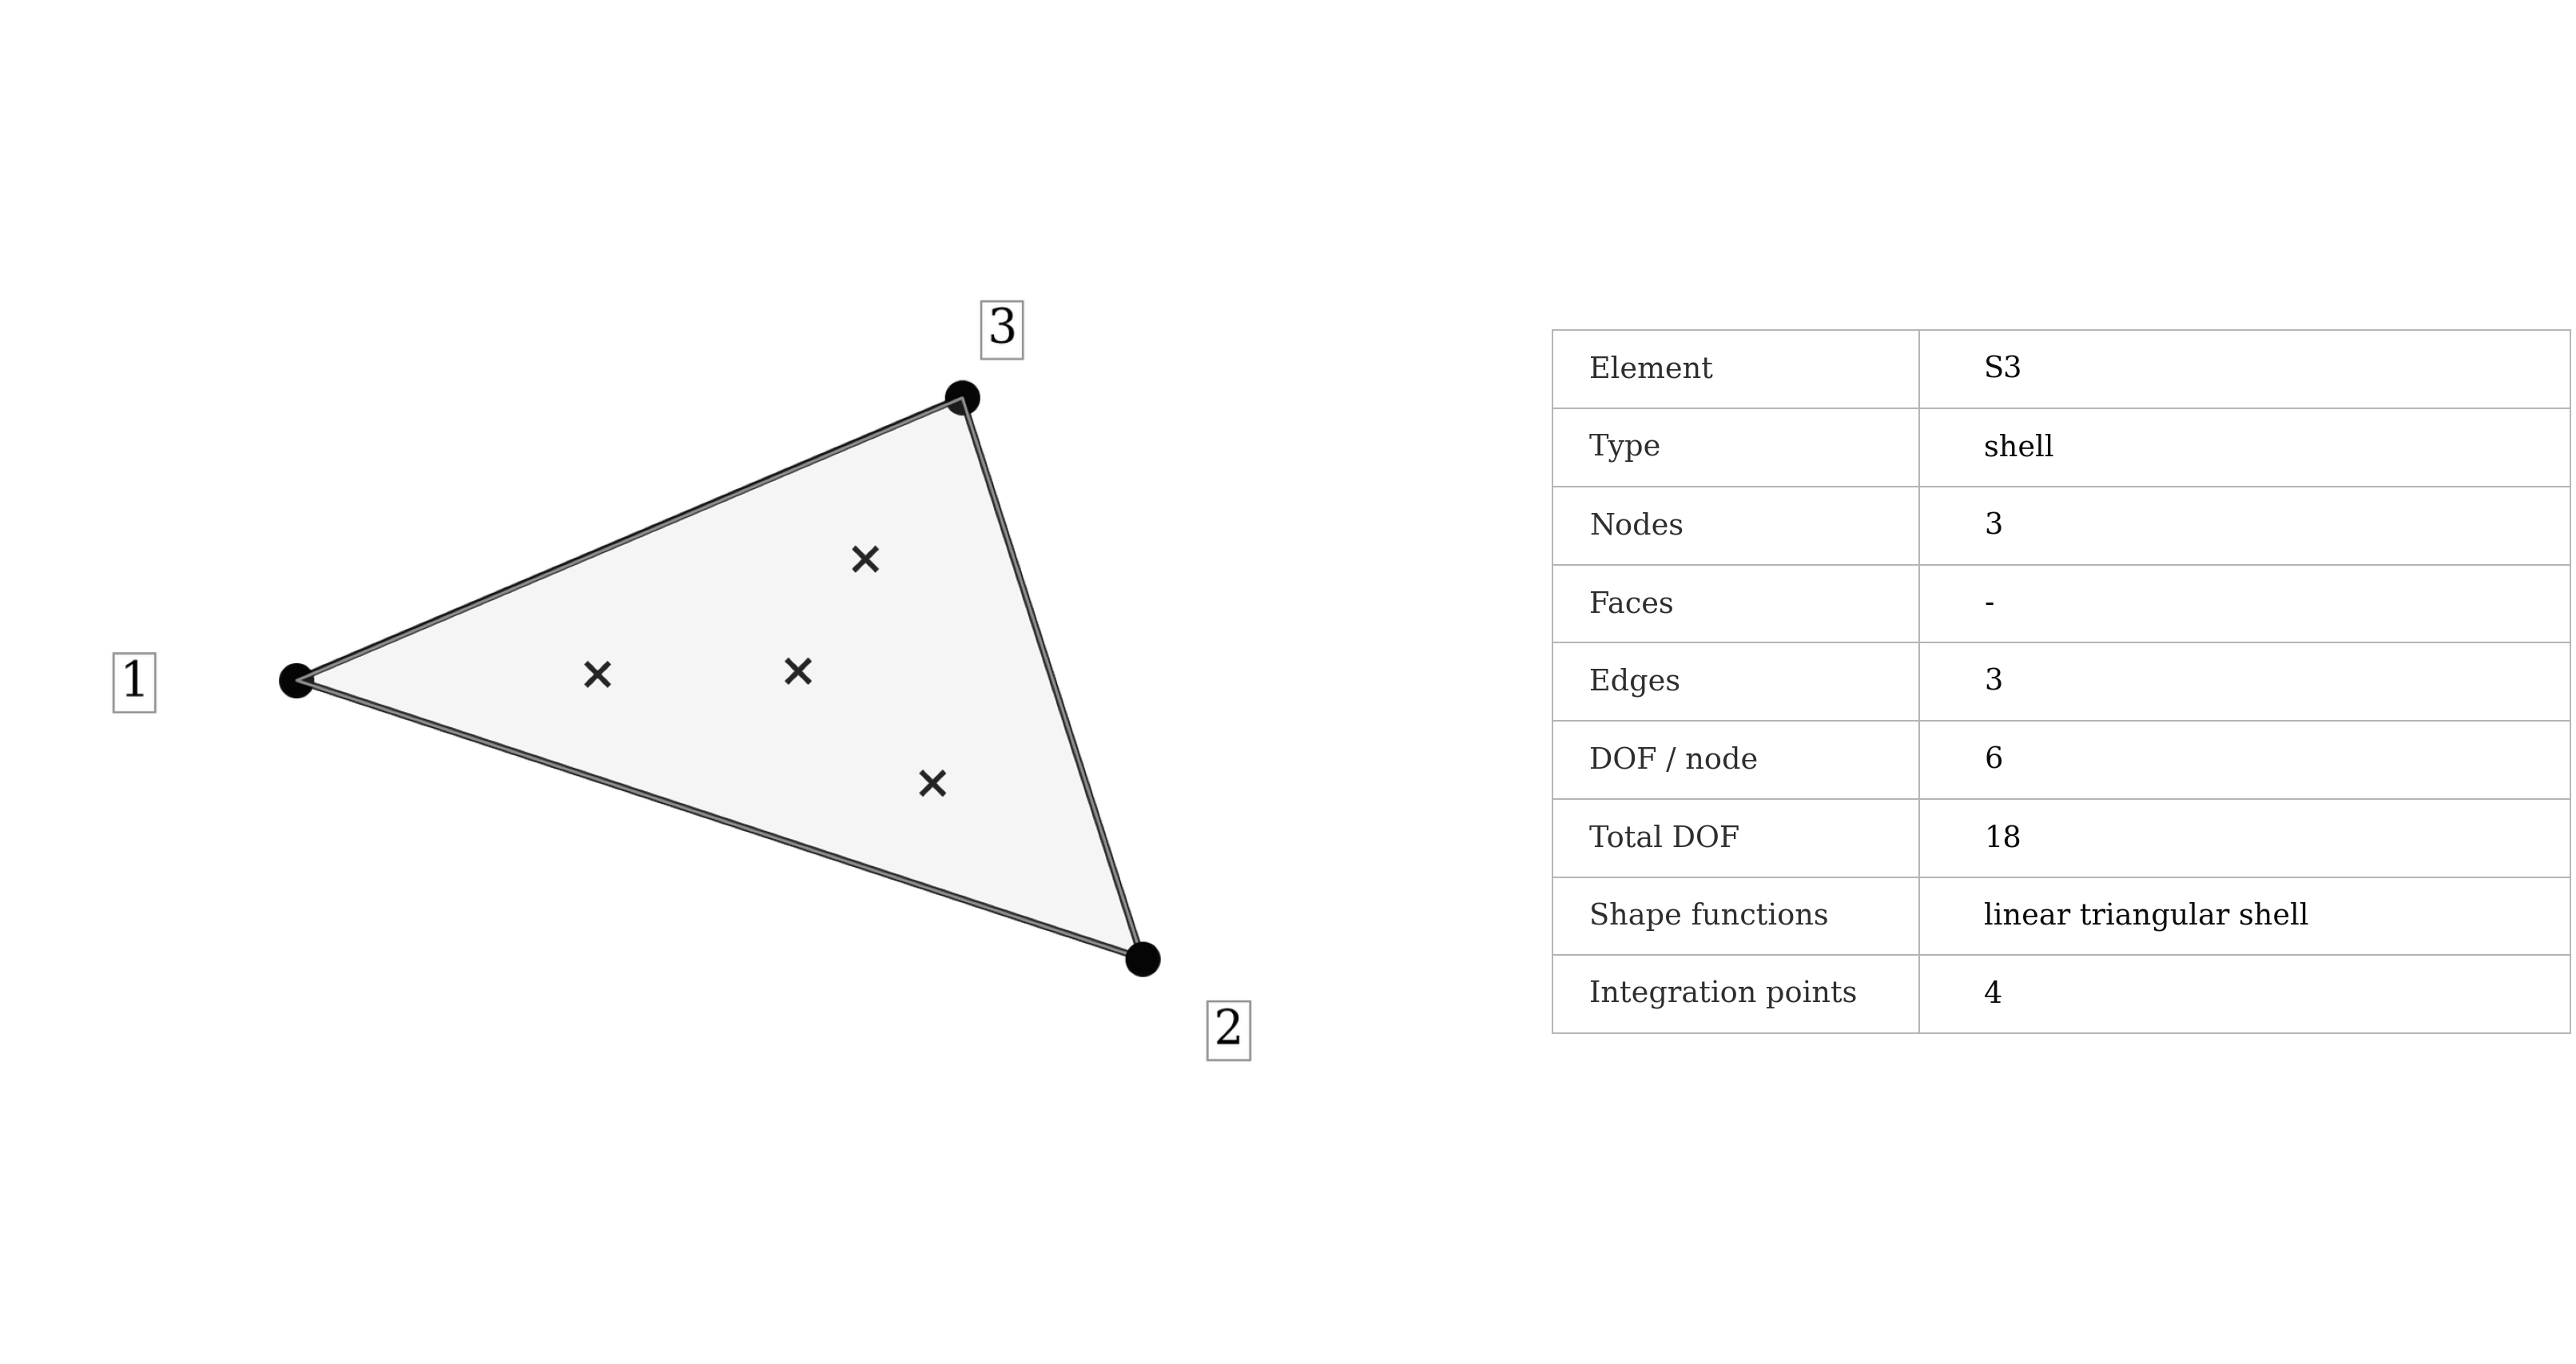
\includegraphics[width=0.76\linewidth]{pages/figures/element_schematics/s3_schematic.png}
    \caption{\val{S3} triangular shell topology.}
\end{figure}

\begin{syntax}
*ELEMENT, TYPE=S3, ELSET=<set>
<id>, <n1>, <n2>, <n3>
\end{syntax}

Native \val{S3} is the legacy three-node triangular shell. Triangular topology is useful for filling irregular surface meshes and transition regions, but a three-node triangle provides only low-order interpolation and typically needs a finer mesh than a good quadrilateral discretization for smooth bending fields.

The element remains accepted so older FEMaster decks continue to run and so legacy formulations can be compared with newer shells. For new work, use \val{MITC3FRT} instead. This recommendation is especially strong for geometrically nonlinear analyses and for models where finite rotations are expected.

Triangular shell meshes should avoid extremely acute angles, abrupt size changes, and inconsistent normal orientation. A dense mesh of poor triangles can still give inferior bending behaviour compared with a smaller set of well-shaped elements.

\clearpage
\section{\val{MITC3FRT}: finite-rotation 3-node shell}

\begin{figure}[H]
    \centering
    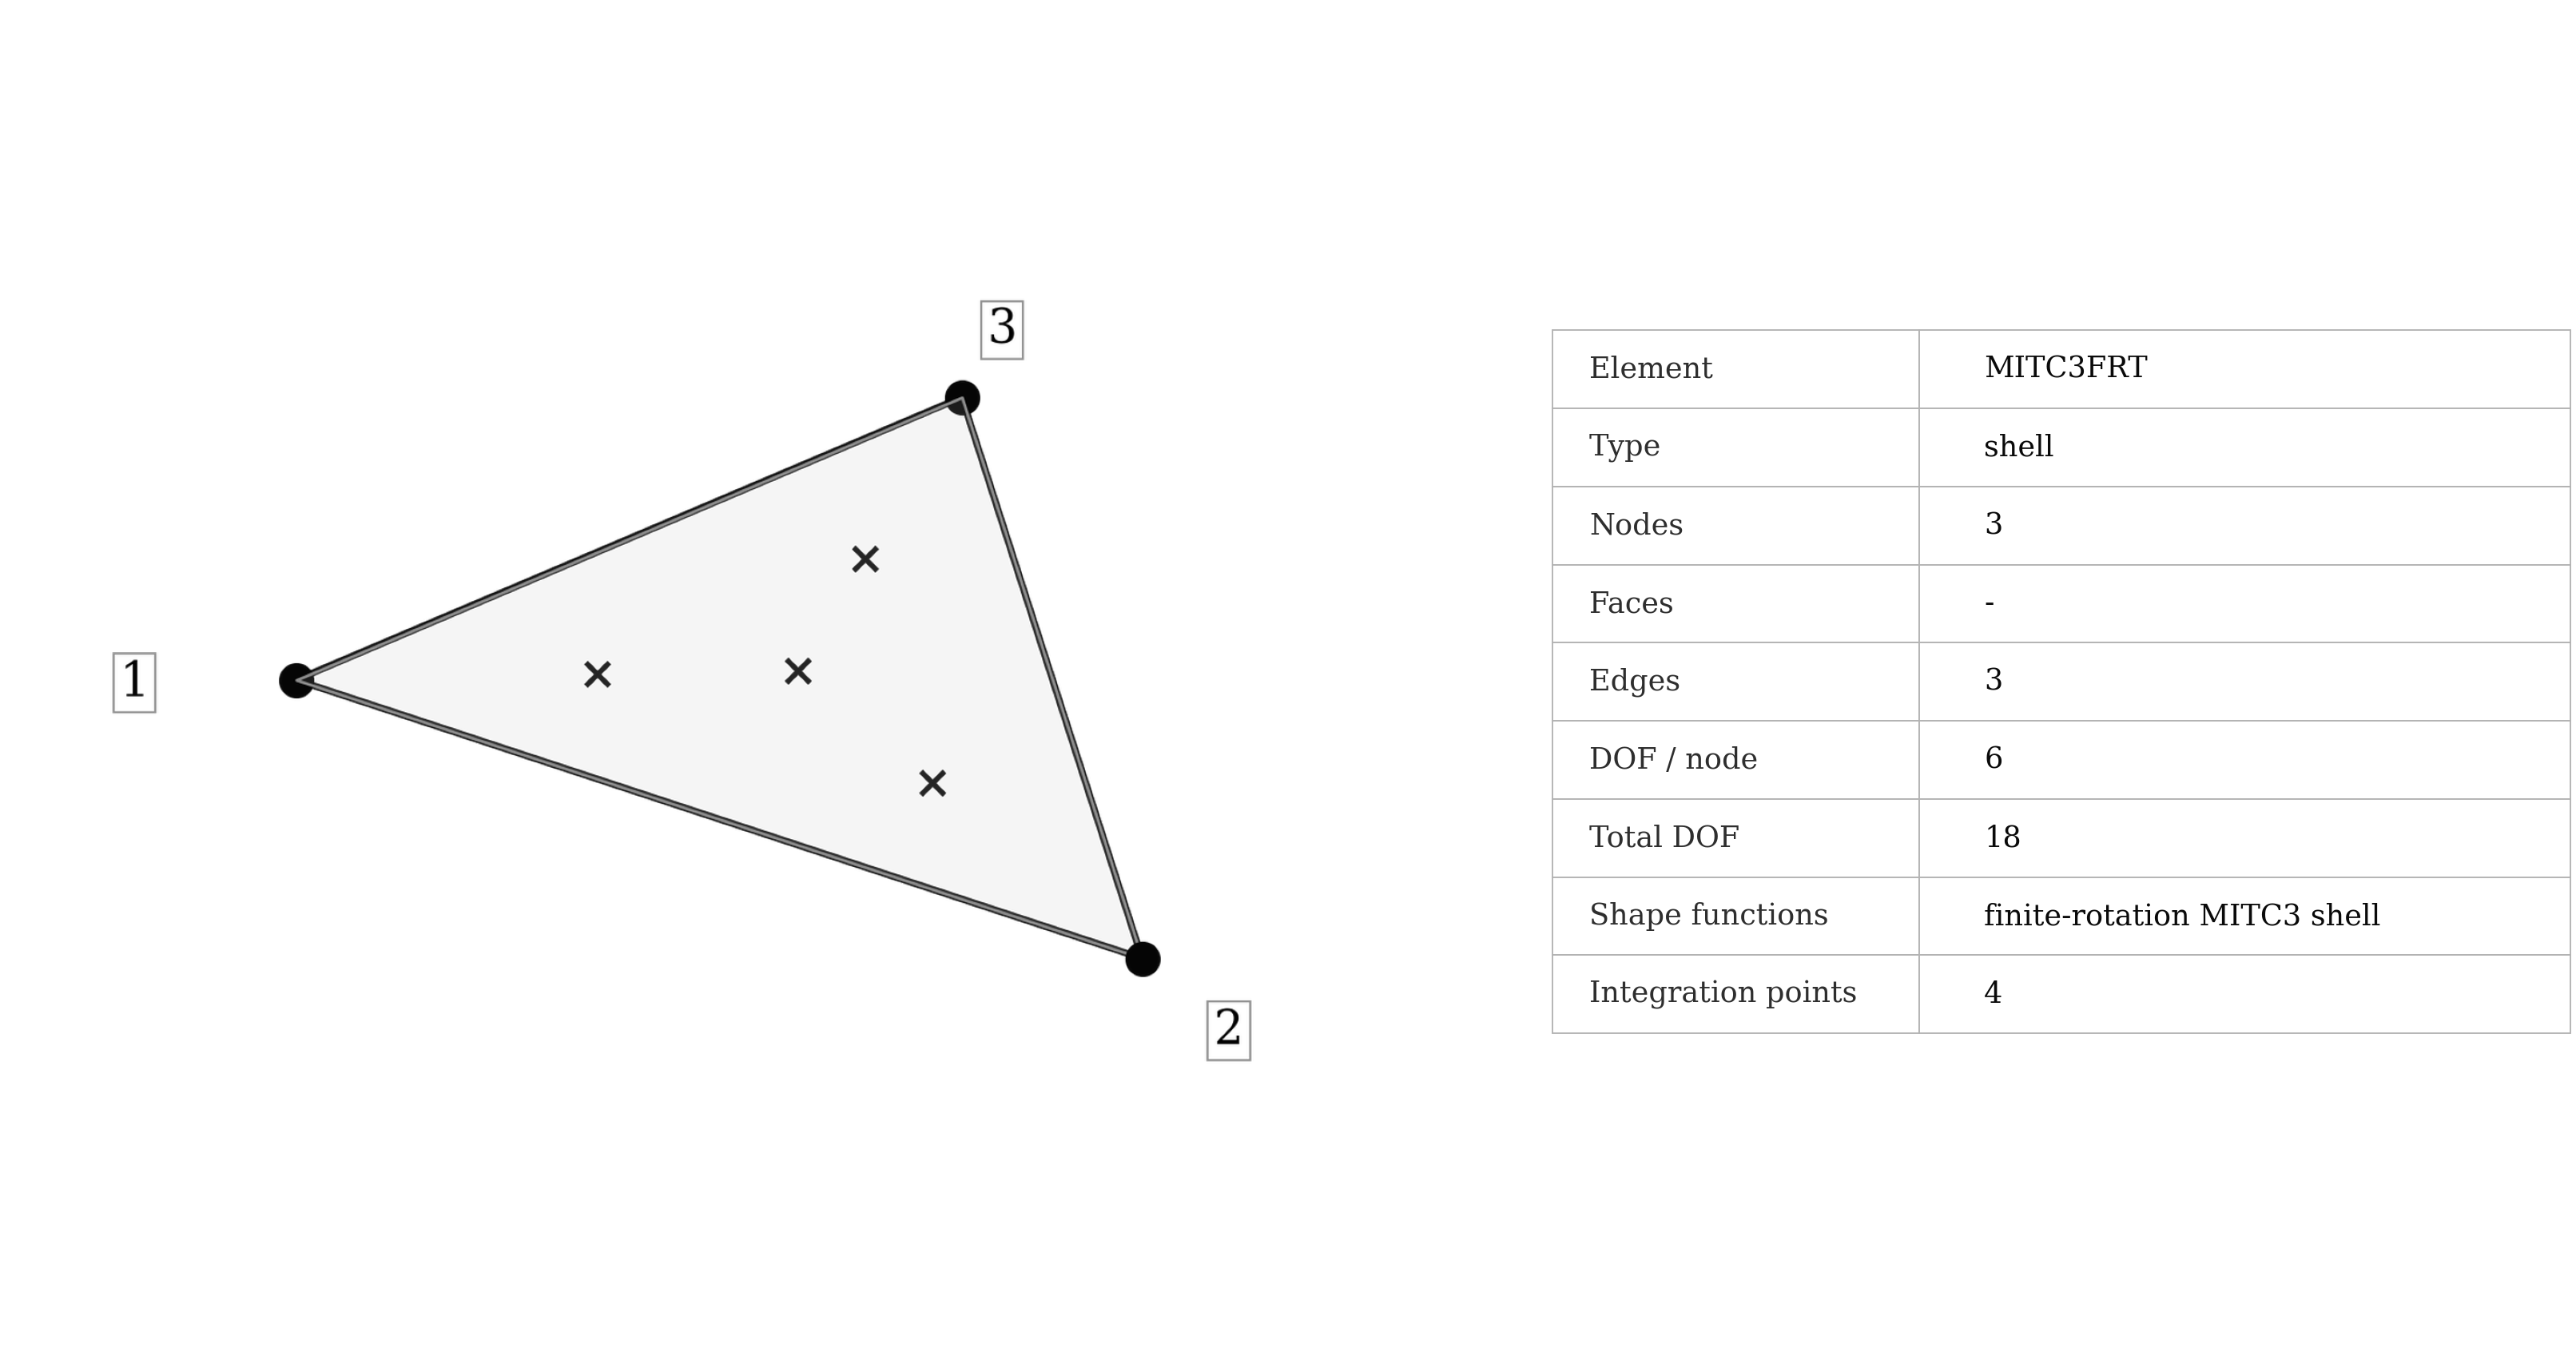
\includegraphics[width=0.76\linewidth]{pages/figures/element_schematics/mitc3frt_schematic.png}
    \caption{\val{MITC3FRT} finite-rotation triangular shell.}
\end{figure}

\begin{syntax}
*ELEMENT, TYPE=MITC3FRT, ELSET=<set>
<id>, <n1>, <n2>, <n3>
\end{syntax}

\val{MITC3FRT} is the current three-node finite-rotation shell formulation. It retains the geometric flexibility of triangular shell meshes while using the FRT shell kinematics intended for geometrically nonlinear analysis.

Use it where triangular topology is unavoidable or convenient: irregular shell boundaries, local mesh transitions, complex curved midsurfaces, and imported surface meshes. As with every three-node shell, convergence in bending-dominated regions generally requires more elements than a high-quality quadrilateral mesh.

For imported Abaqus input, both \val{S3} and \val{S3R} are translated to this formulation. The Abaqus suffix therefore does not select a separate reduced-integration implementation inside FEMaster.

\clearpage
\section{\val{S4}: legacy 4-node quadrilateral shell}

\begin{figure}[H]
    \centering
    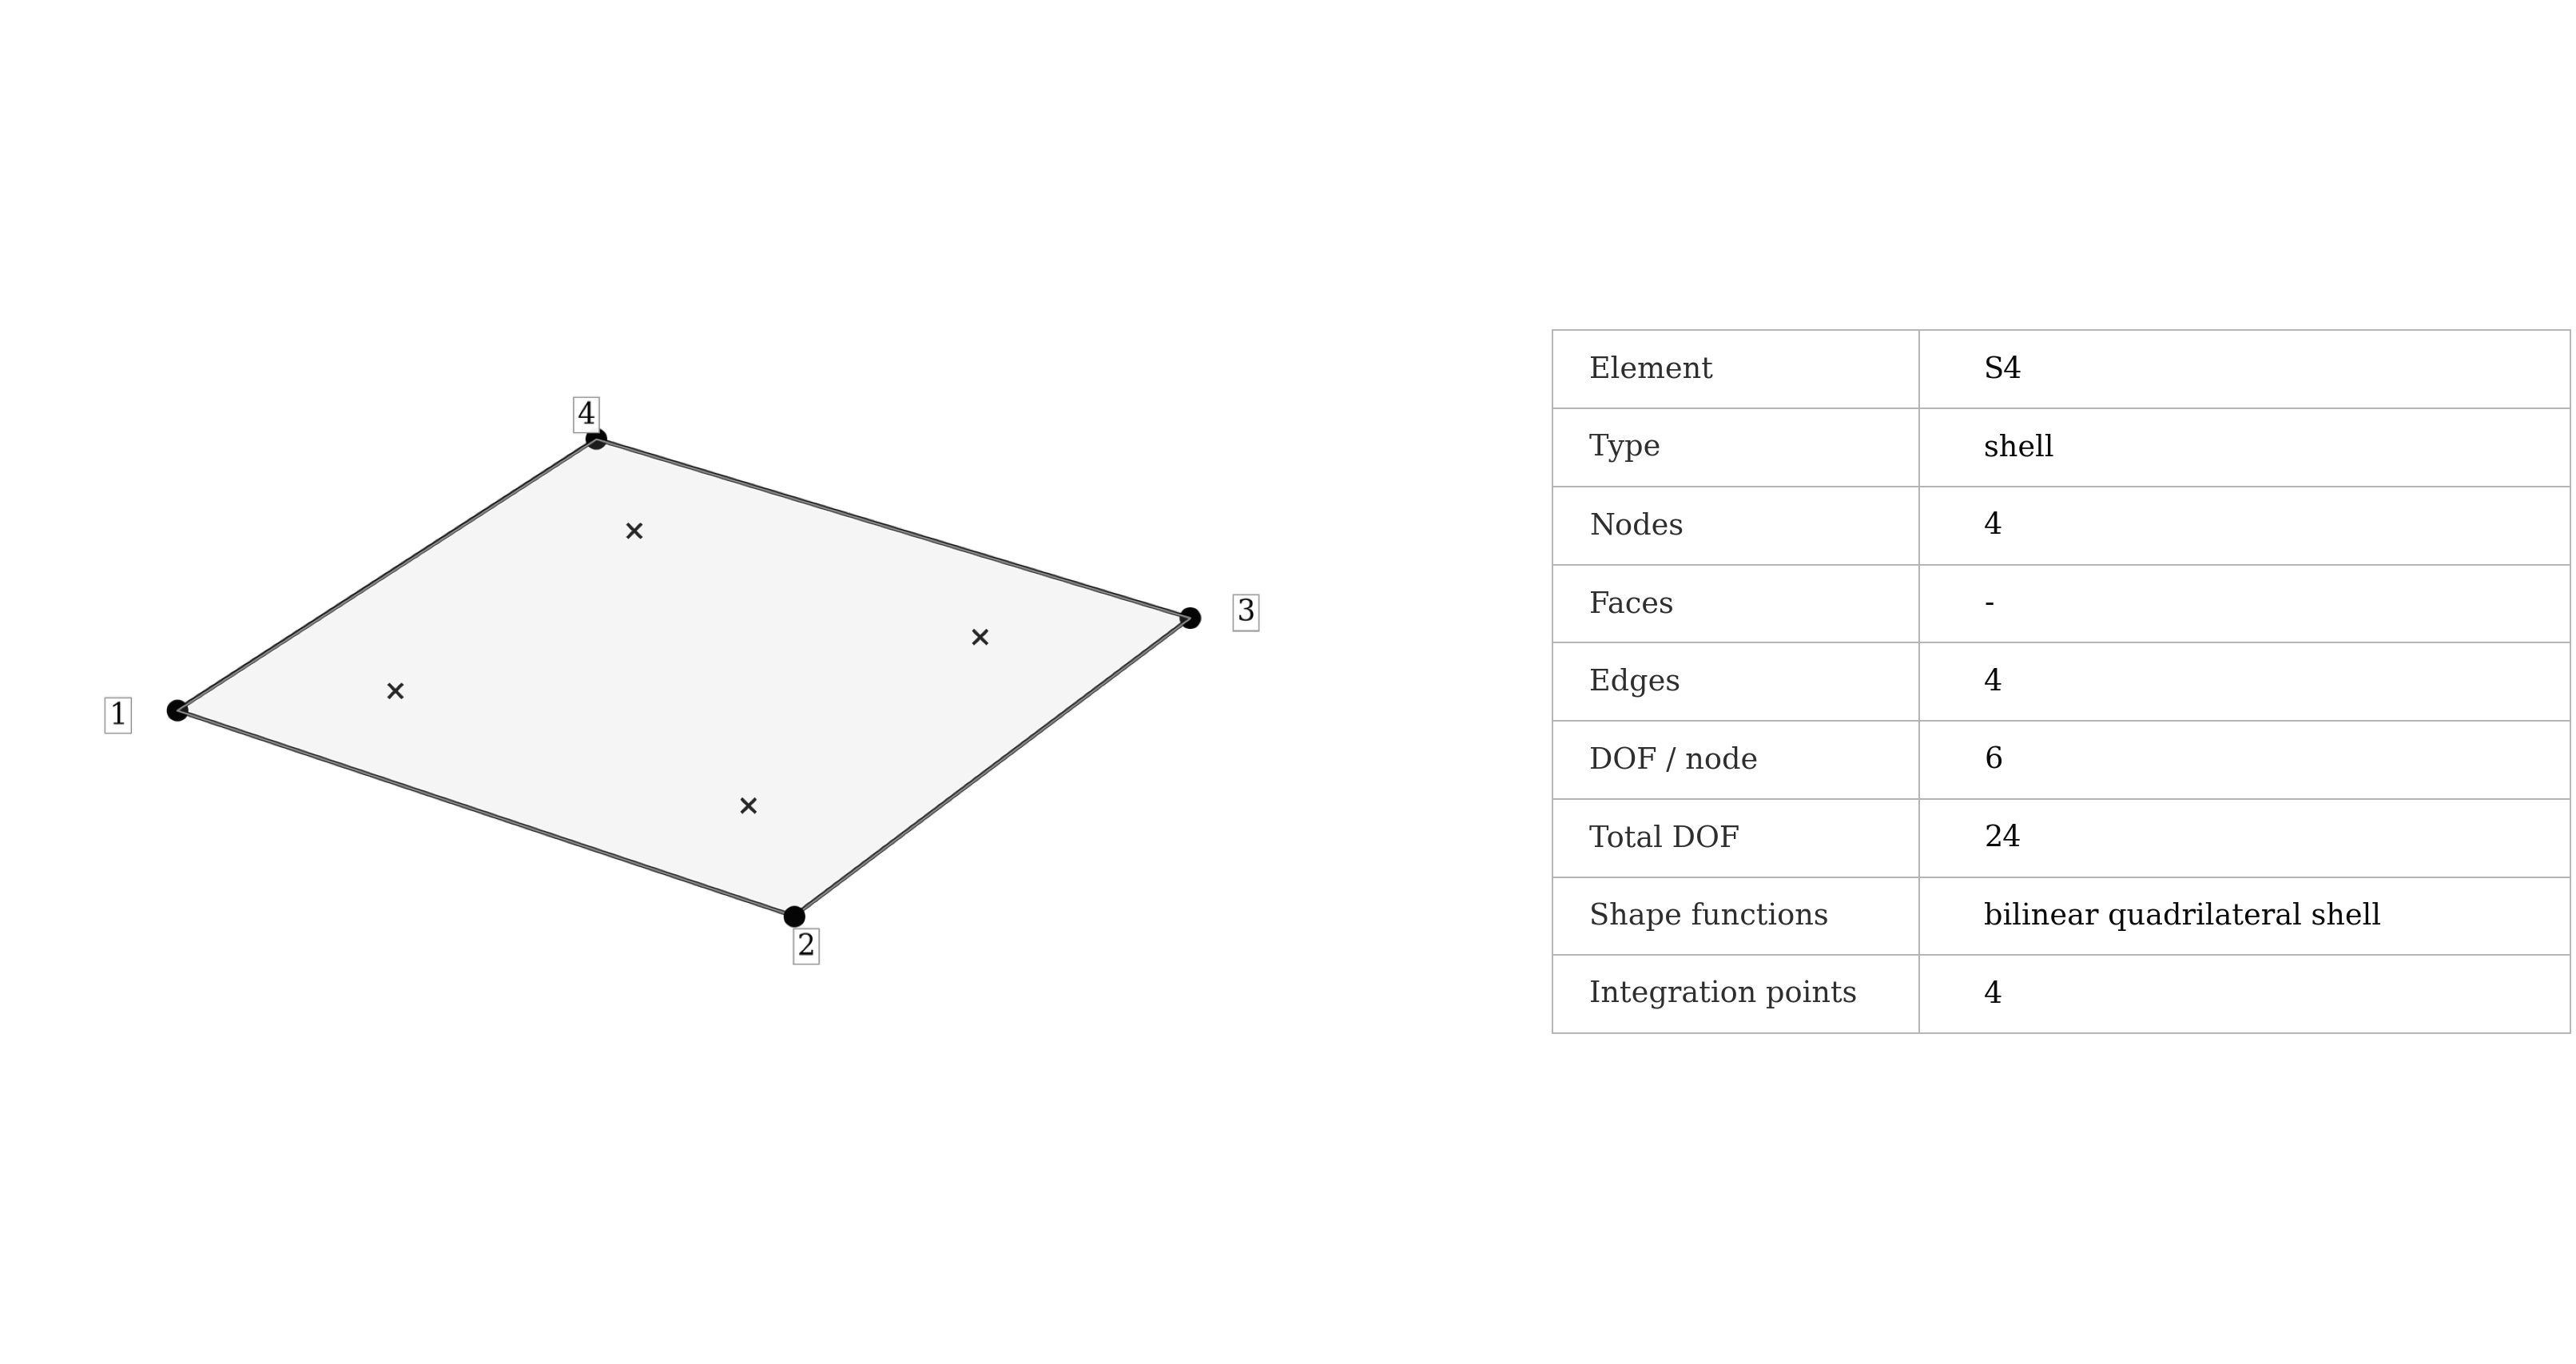
\includegraphics[width=0.78\linewidth]{pages/figures/element_schematics/s4_schematic.png}
    \caption{\val{S4} quadrilateral shell topology.}
\end{figure}

\begin{syntax}
*ELEMENT, TYPE=S4, ELSET=<set>
<id>, <n1>, <n2>, <n3>, <n4>
\end{syntax}

Native \val{S4} is the legacy four-node quadrilateral shell. Quadrilateral topology is attractive for plates, webs, skins, and other surfaces with two natural in-plane directions, but this specific legacy formulation should not be the default for new FEMaster models.

The low-order formulation can suffer severe transverse-shear locking in thin bending-dominated problems. A coarse \val{S4} mesh may therefore appear dramatically too stiff while still satisfying equilibrium. Refining the mesh reduces this problem but is generally less efficient than choosing an appropriate MITC formulation.

Use \val{MITC4FRT} for new four-node shell models. Keep \val{S4} for compatibility, regression comparisons, or controlled studies of the legacy formulation.

\clearpage
\section{\val{MITC4}: legacy 4-node shell with tied shear interpolation}

\begin{figure}[H]
    \centering
    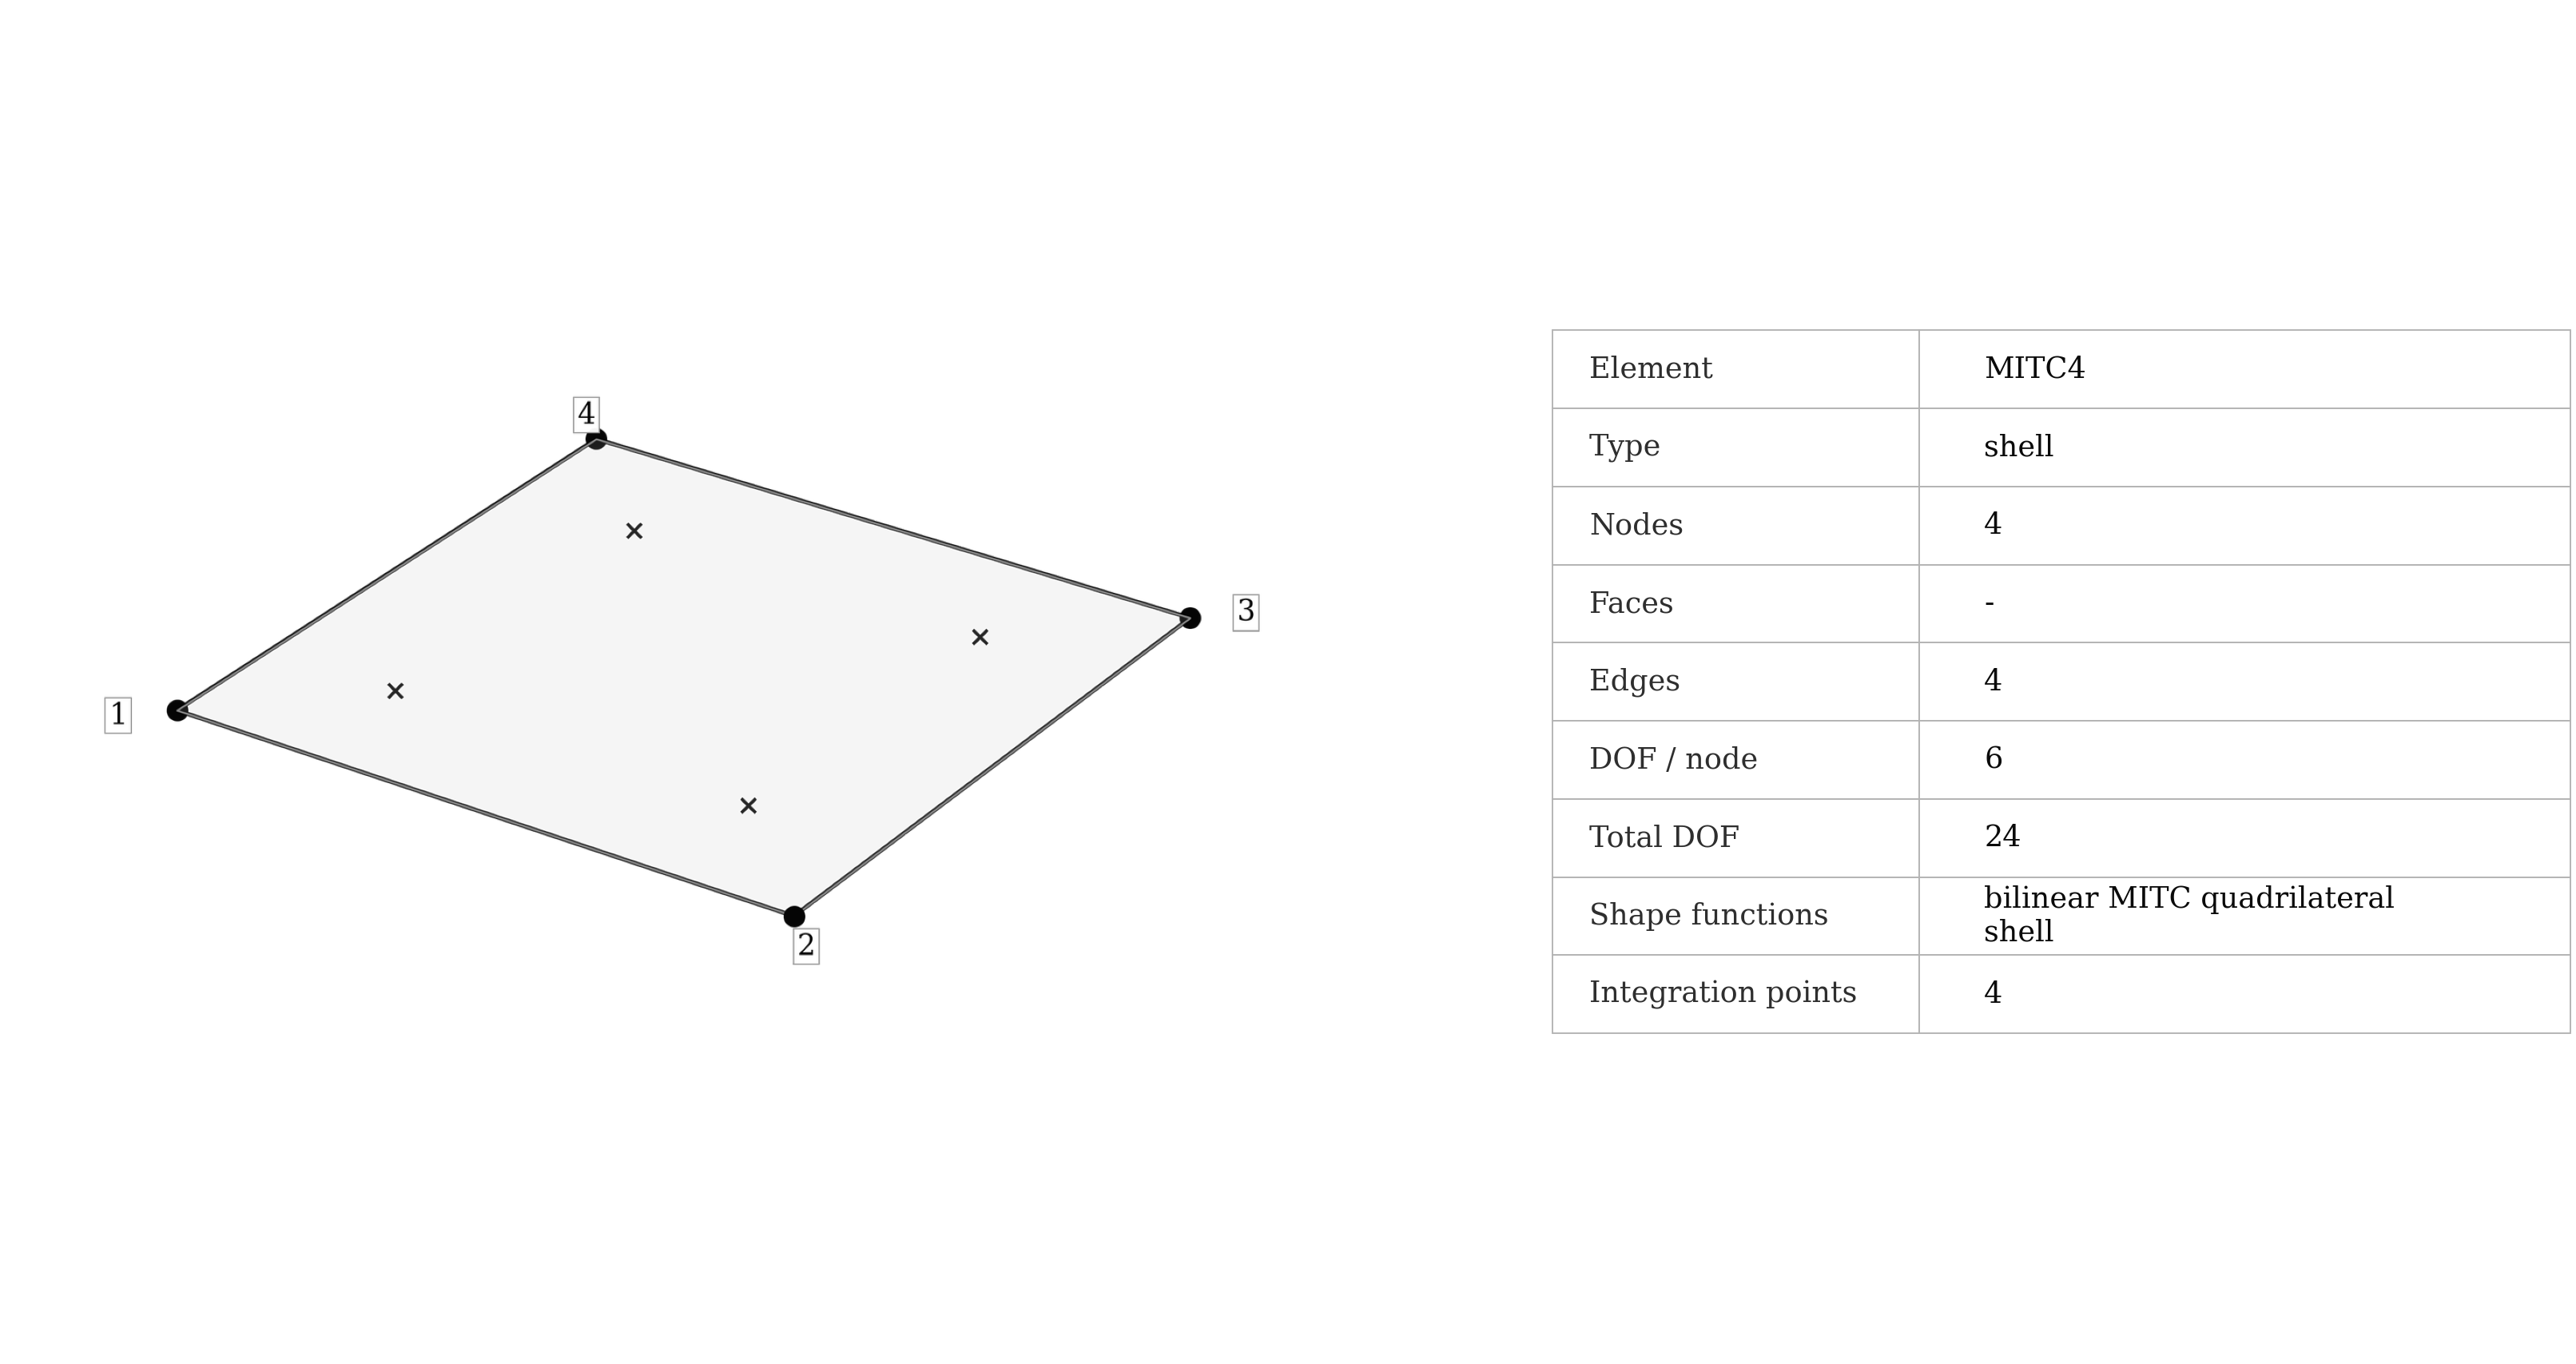
\includegraphics[width=0.78\linewidth]{pages/figures/element_schematics/mitc4_schematic.png}
    \caption{\val{MITC4} shell with MITC transverse-shear interpolation.}
\end{figure}

\begin{syntax}
*ELEMENT, TYPE=MITC4, ELSET=<set>
<id>, <n1>, <n2>, <n3>, <n4>
\end{syntax}

\val{MITC4} uses the same four-node topology as \val{S4} but replaces the direct low-order transverse-shear interpolation with MITC-style tied shear interpolation. The purpose is to suppress the artificial shear constraint responsible for locking in thin bending problems.

This element historically provided much better thin-shell bending behaviour than \val{S4} on coarse meshes. It remains useful for regression and linear-formulation comparison, but new models should normally use \val{MITC4FRT}, which combines the corresponding low-order MITC idea with the current finite-rotation shell formulation.

MITC interpolation does not make a quadrilateral insensitive to mesh quality. Excessive warping, skew, poor aspect ratio, and inconsistent normals can still degrade both stiffness and stress recovery.

\clearpage
\section{\val{MITC4FRT}: finite-rotation 4-node MITC shell}

\begin{figure}[H]
    \centering
    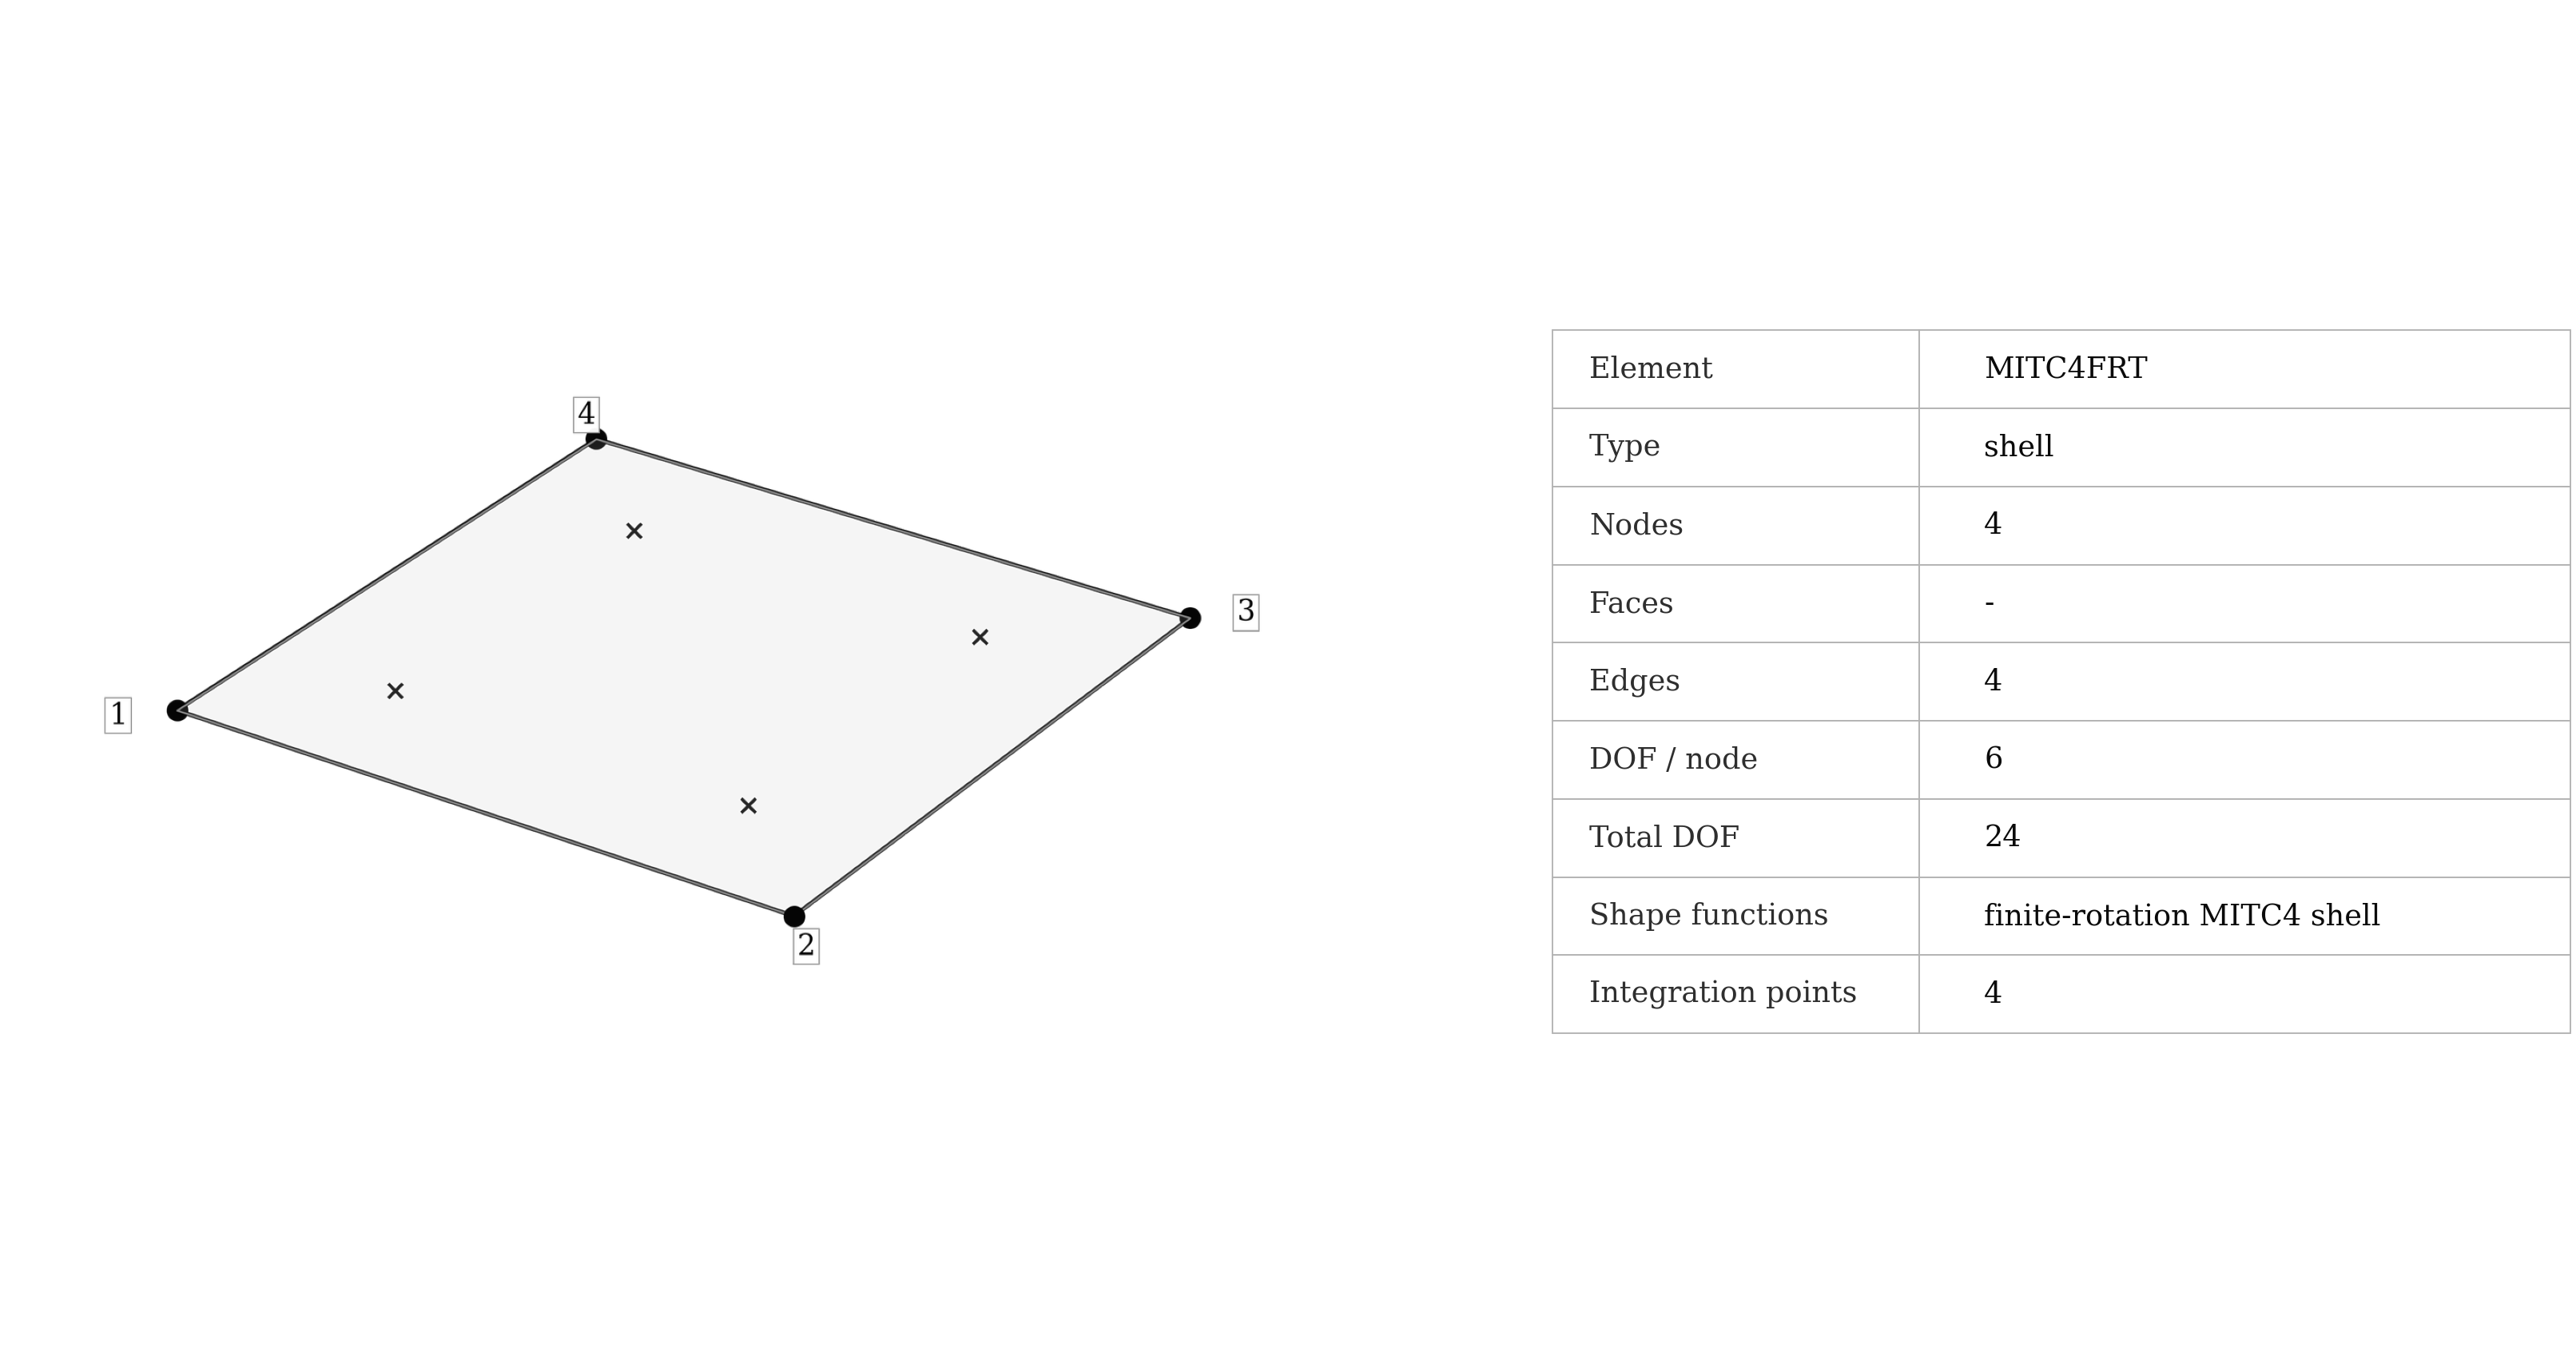
\includegraphics[width=0.78\linewidth]{pages/figures/element_schematics/mitc4frt_schematic.png}
    \caption{\val{MITC4FRT} finite-rotation quadrilateral shell.}
\end{figure}

\begin{syntax}
*ELEMENT, TYPE=MITC4FRT, ELSET=<set>
<id>, <n1>, <n2>, <n3>, <n4>
\end{syntax}

\val{MITC4FRT} is the recommended low-order quadrilateral shell for current FEMaster models. It uses finite-rotation shell kinematics and MITC transverse-shear interpolation, making it suitable for thin-shell bending as well as geometrically nonlinear deformation where rotations become large.

The four-node topology keeps mesh generation and element cost modest. It is a good default for panels, webs, skins, shells of moderate curvature, and large shell assemblies when a structured or mostly quadrilateral midsurface mesh is available.

Tied shear interpolation addresses shear locking but does not eliminate geometric discretization error. Curved surfaces still require sufficient mesh density, strongly warped quadrilaterals should be avoided, and nonlinear load paths should be checked using deformed shapes, reaction balance, and convergence under refinement.

The supported Abaqus labels \val{S4} and \val{S4R} are both translated to \val{MITC4FRT}.

\clearpage
\section{\val{S6}: legacy 6-node triangular shell}

\begin{figure}[H]
    \centering
    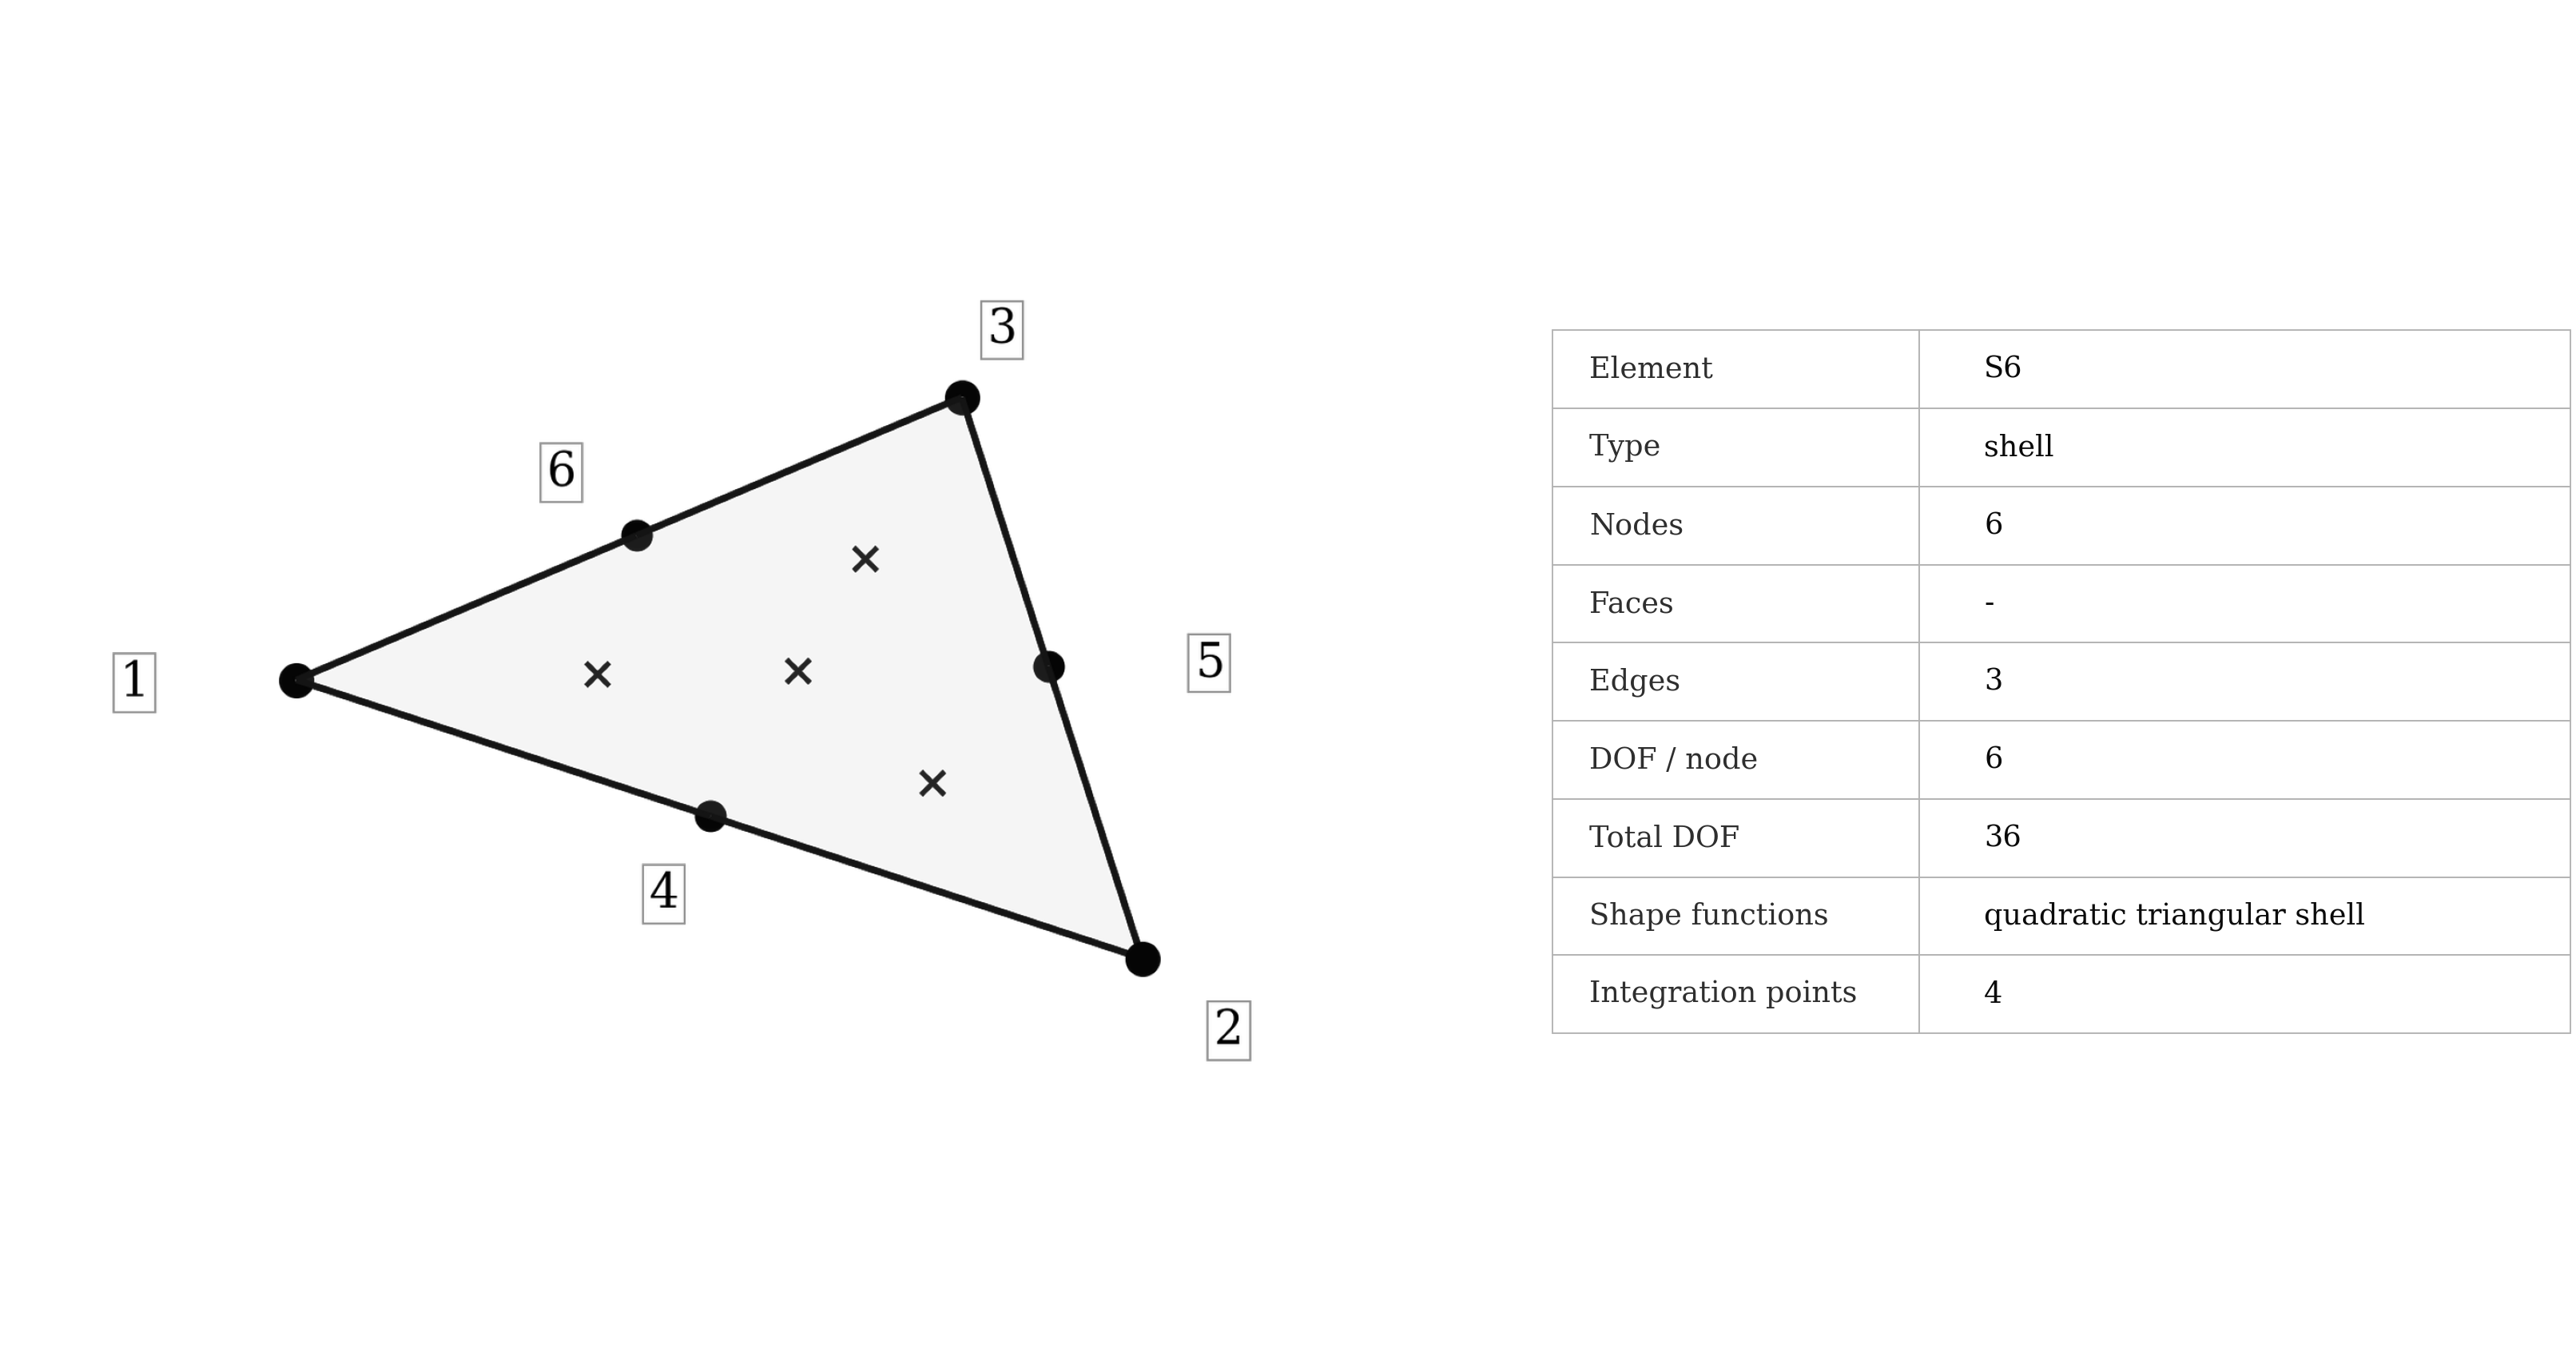
\includegraphics[width=0.78\linewidth]{pages/figures/element_schematics/s6_schematic.png}
    \caption{\val{S6} quadratic triangular shell.}
\end{figure}

\begin{syntax}
*ELEMENT, TYPE=S6, ELSET=<set>
<id>, <n1>, <n2>, <n3>, <n4>, <n5>, <n6>
\end{syntax}

Native \val{S6} is the legacy six-node quadratic triangular shell. The midside nodes improve geometric representation and allow a smoother in-plane and bending interpolation than \val{S3}. It is useful in older curved triangular shell meshes and for comparisons with the corresponding FRT formulation.

For new analyses, use \val{MITC6FRT}. The higher-order triangle can represent curved boundaries effectively, but the location of midside nodes and the quality of the parent triangle remain important. Badly curved or highly skewed elements can create poor mappings despite the higher interpolation order.

\clearpage
\section{\val{MITC6FRT}: finite-rotation 6-node shell}

\begin{figure}[H]
    \centering
    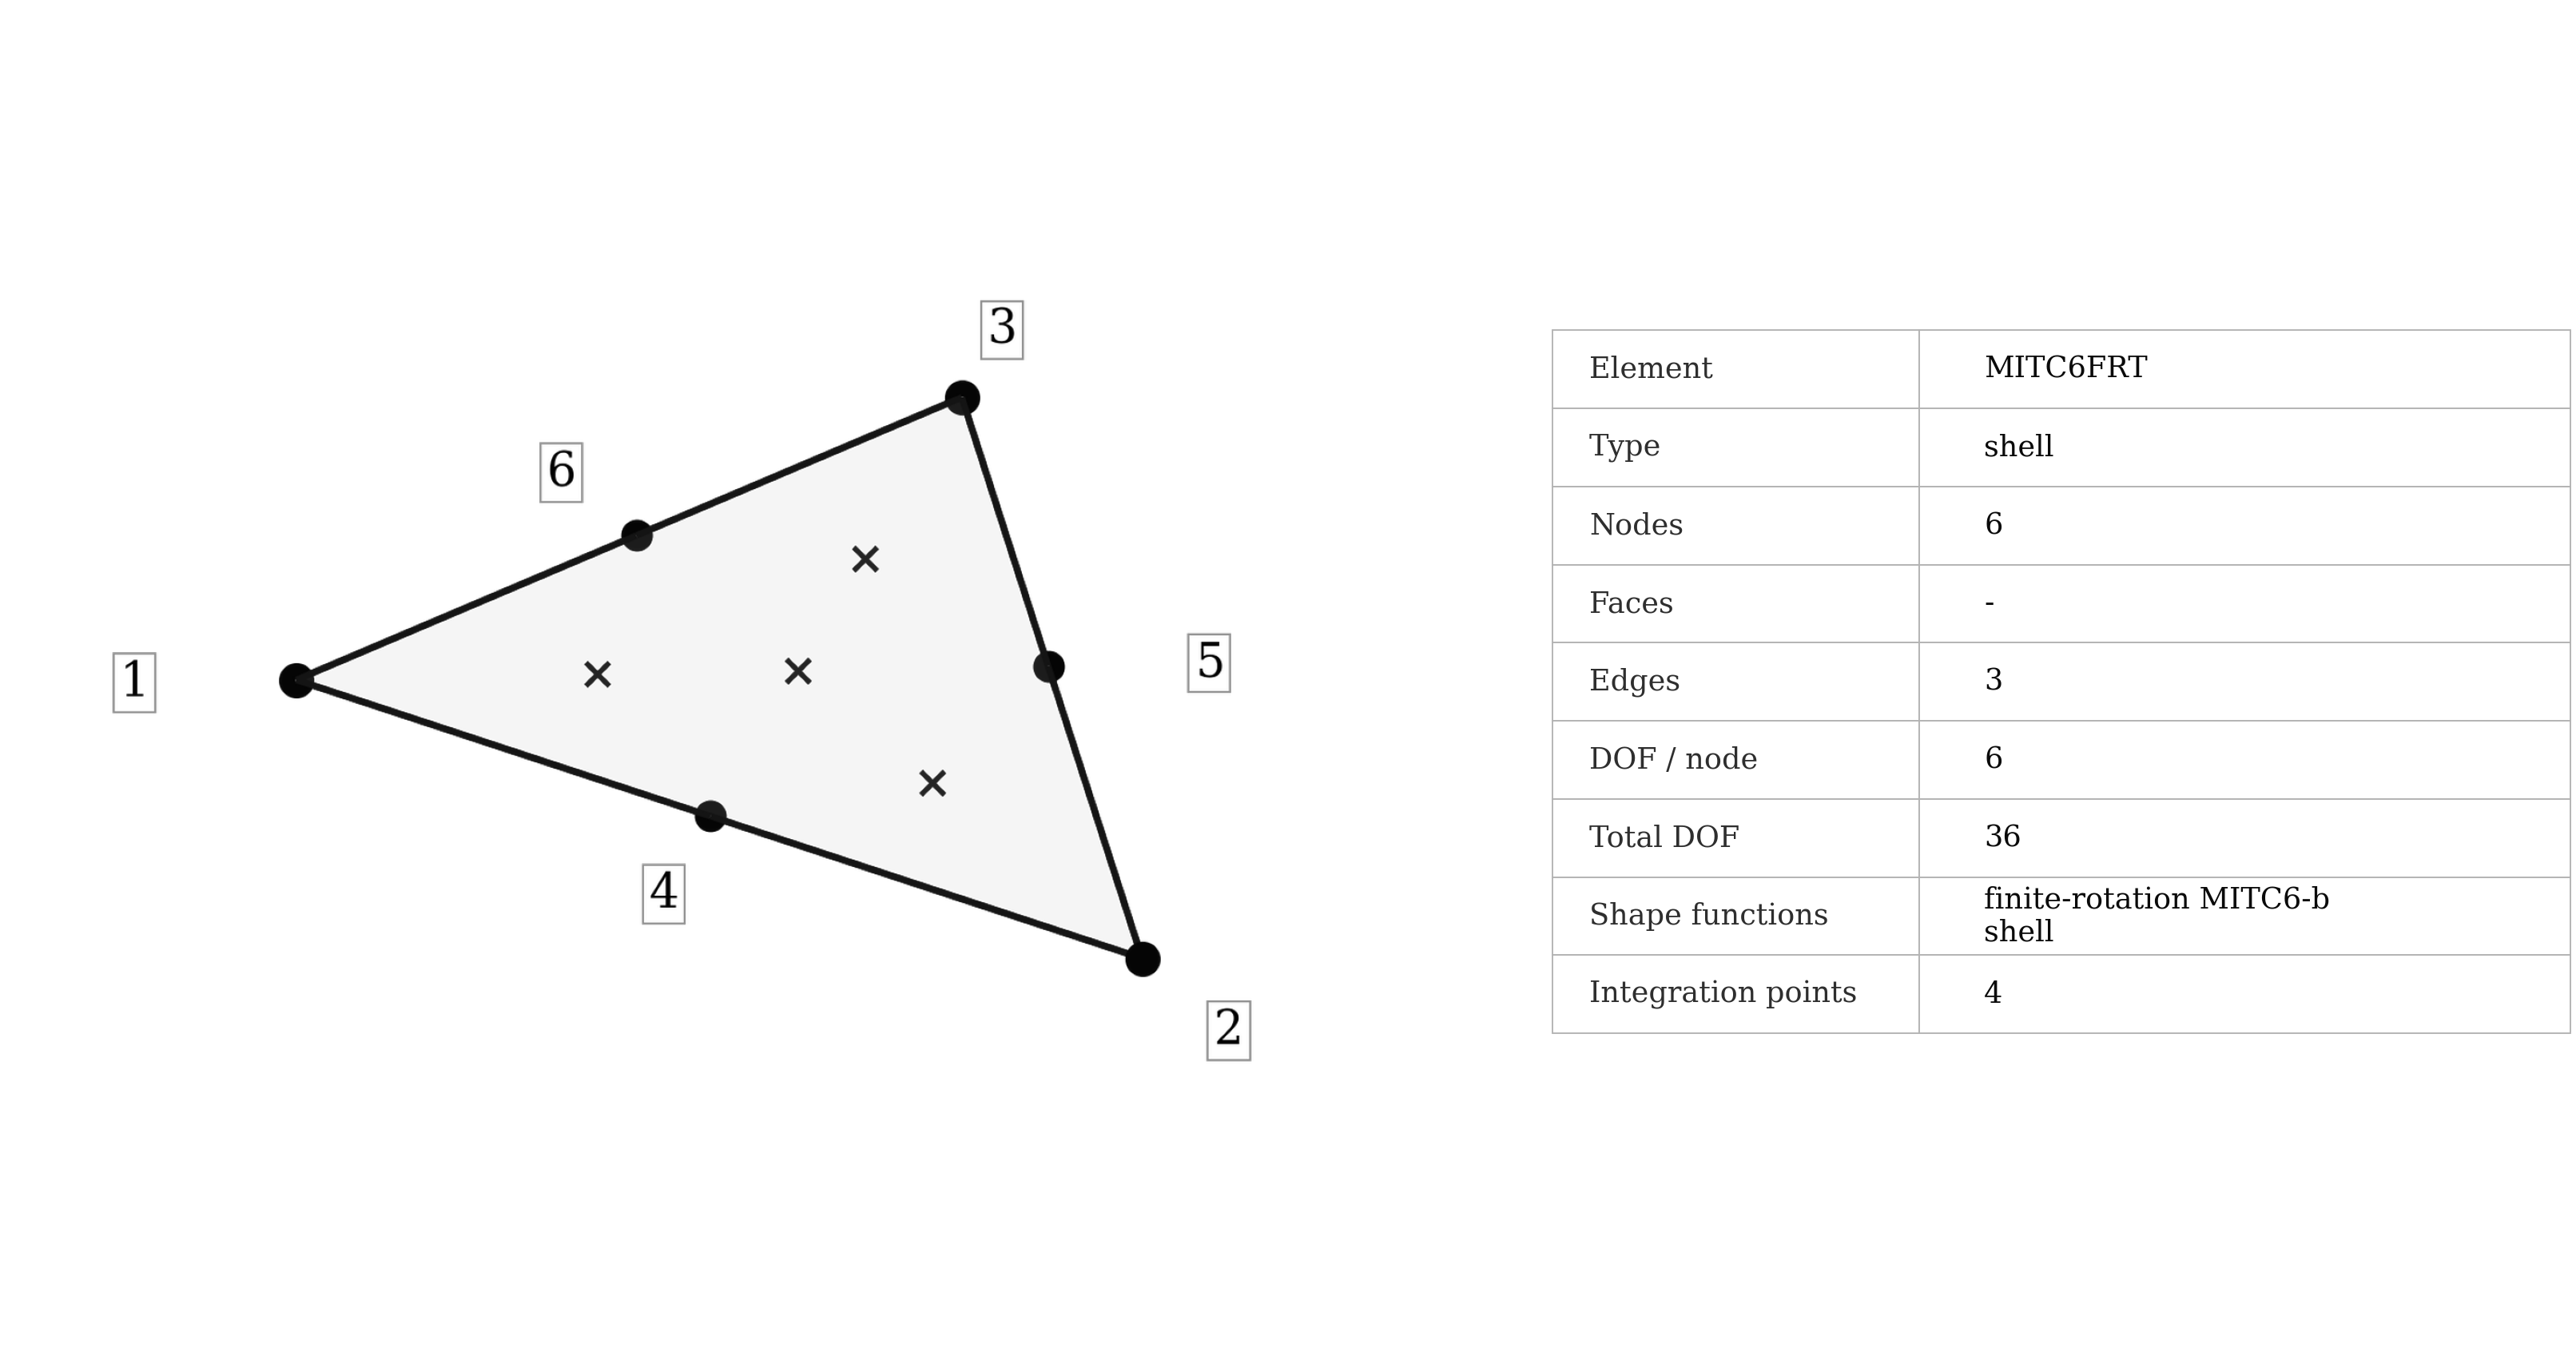
\includegraphics[width=0.78\linewidth]{pages/figures/element_schematics/mitc6frt_schematic.png}
    \caption{\val{MITC6FRT} finite-rotation six-node triangular shell.}
\end{figure}

\begin{syntax}
*ELEMENT, TYPE=MITC6FRT, ELSET=<set>
<id>, <n1>, <n2>, <n3>, <n4>, <n5>, <n6>
\end{syntax}

\val{MITC6FRT} is the current six-node triangular finite-rotation shell. It combines quadratic triangular geometry with the FRT shell formulation and is the preferred triangular choice when a higher-order midsurface description is desired.

The element is well suited to curved shell regions where triangular topology is convenient but a low-order three-node mesh would require excessive refinement. Midside nodes allow curved edges and smoother deformation fields, provided they are positioned consistently with the intended geometry.

Both Abaqus \val{S6} and \val{S6R} are translated to this formulation by the current reader.

\clearpage
\section{\val{S8}: legacy 8-node quadrilateral shell}

\begin{figure}[H]
    \centering
    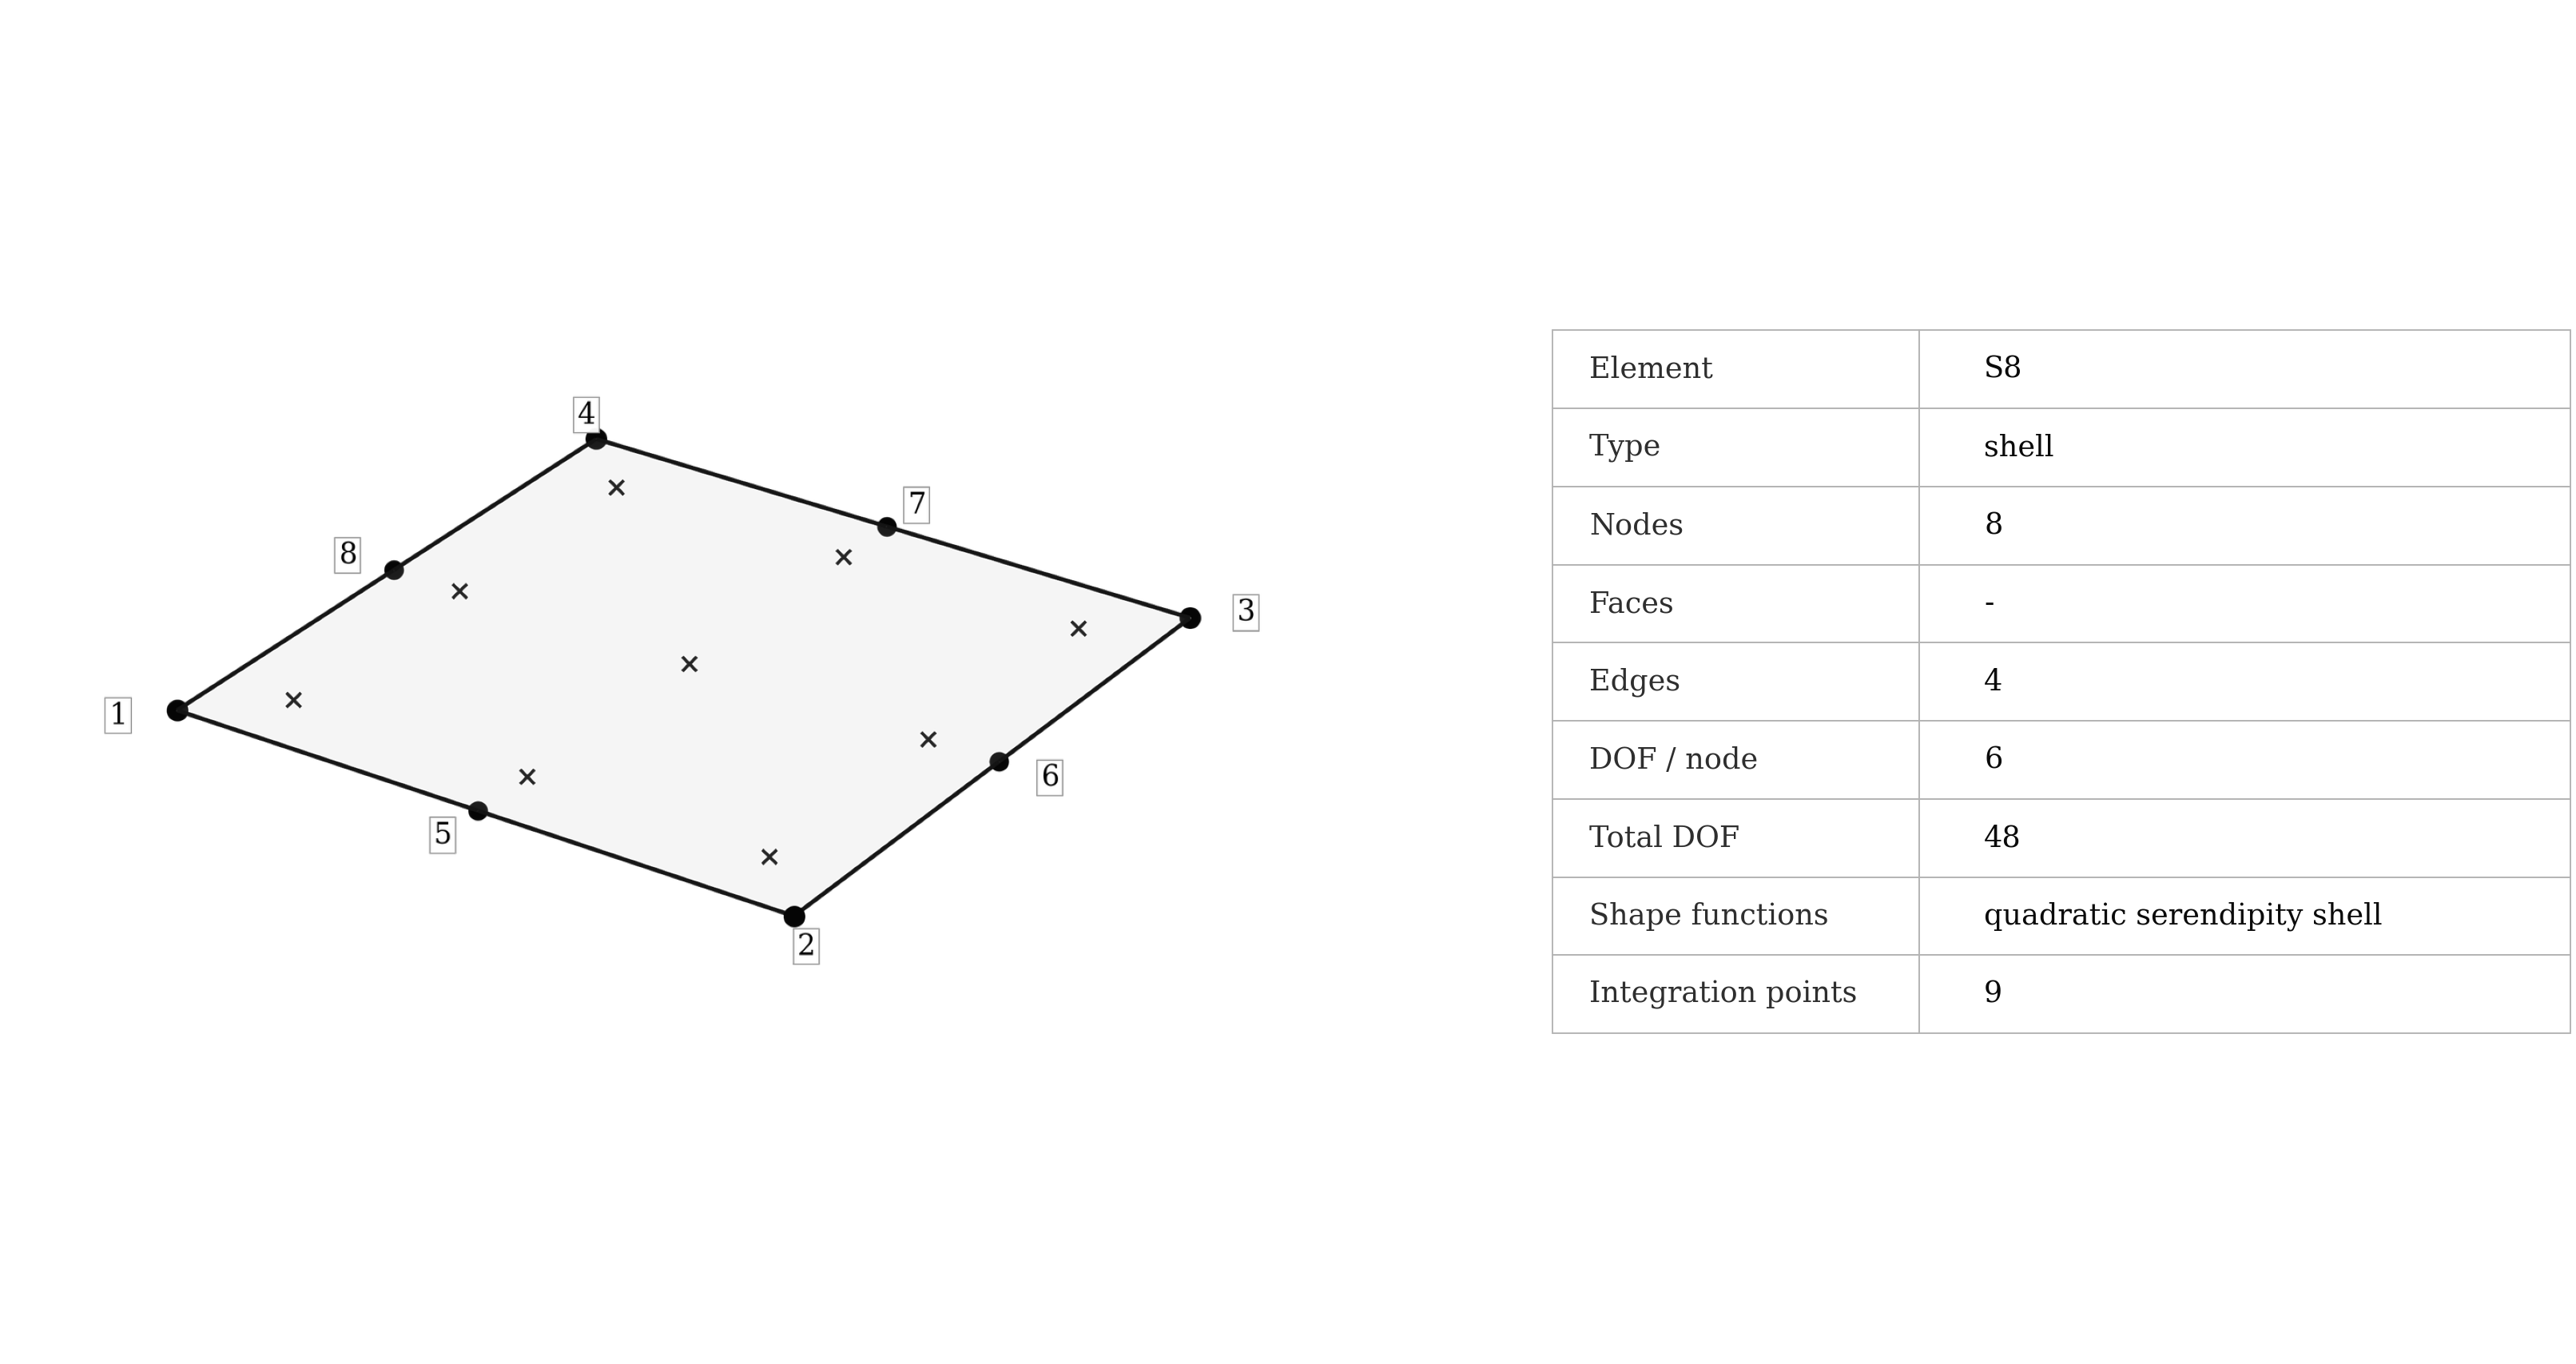
\includegraphics[width=0.80\linewidth]{pages/figures/element_schematics/s8_schematic.png}
    \caption{\val{S8} quadratic quadrilateral shell.}
\end{figure}

\begin{syntax}
*ELEMENT, TYPE=S8, ELSET=<set>
<id>, <n1>, <n2>, <n3>, <n4>, <n5>, <n6>, <n7>, <n8>
\end{syntax}

Native \val{S8} is the legacy eight-node quadratic quadrilateral shell. Four corner nodes and four midside nodes provide a higher-order surface interpolation than \val{S4}. This gives substantially better representation of curved geometry and smooth bending fields when the element is well shaped.

The formulation remains available for older models and comparison studies. For new models, use \val{MITC8FRT}. Higher order does not remove the need for good midside-node placement, reasonable aspect ratio, and controlled warping.

\clearpage
\section{\val{MITC8}: legacy 8-node MITC shell}

\begin{figure}[H]
    \centering
    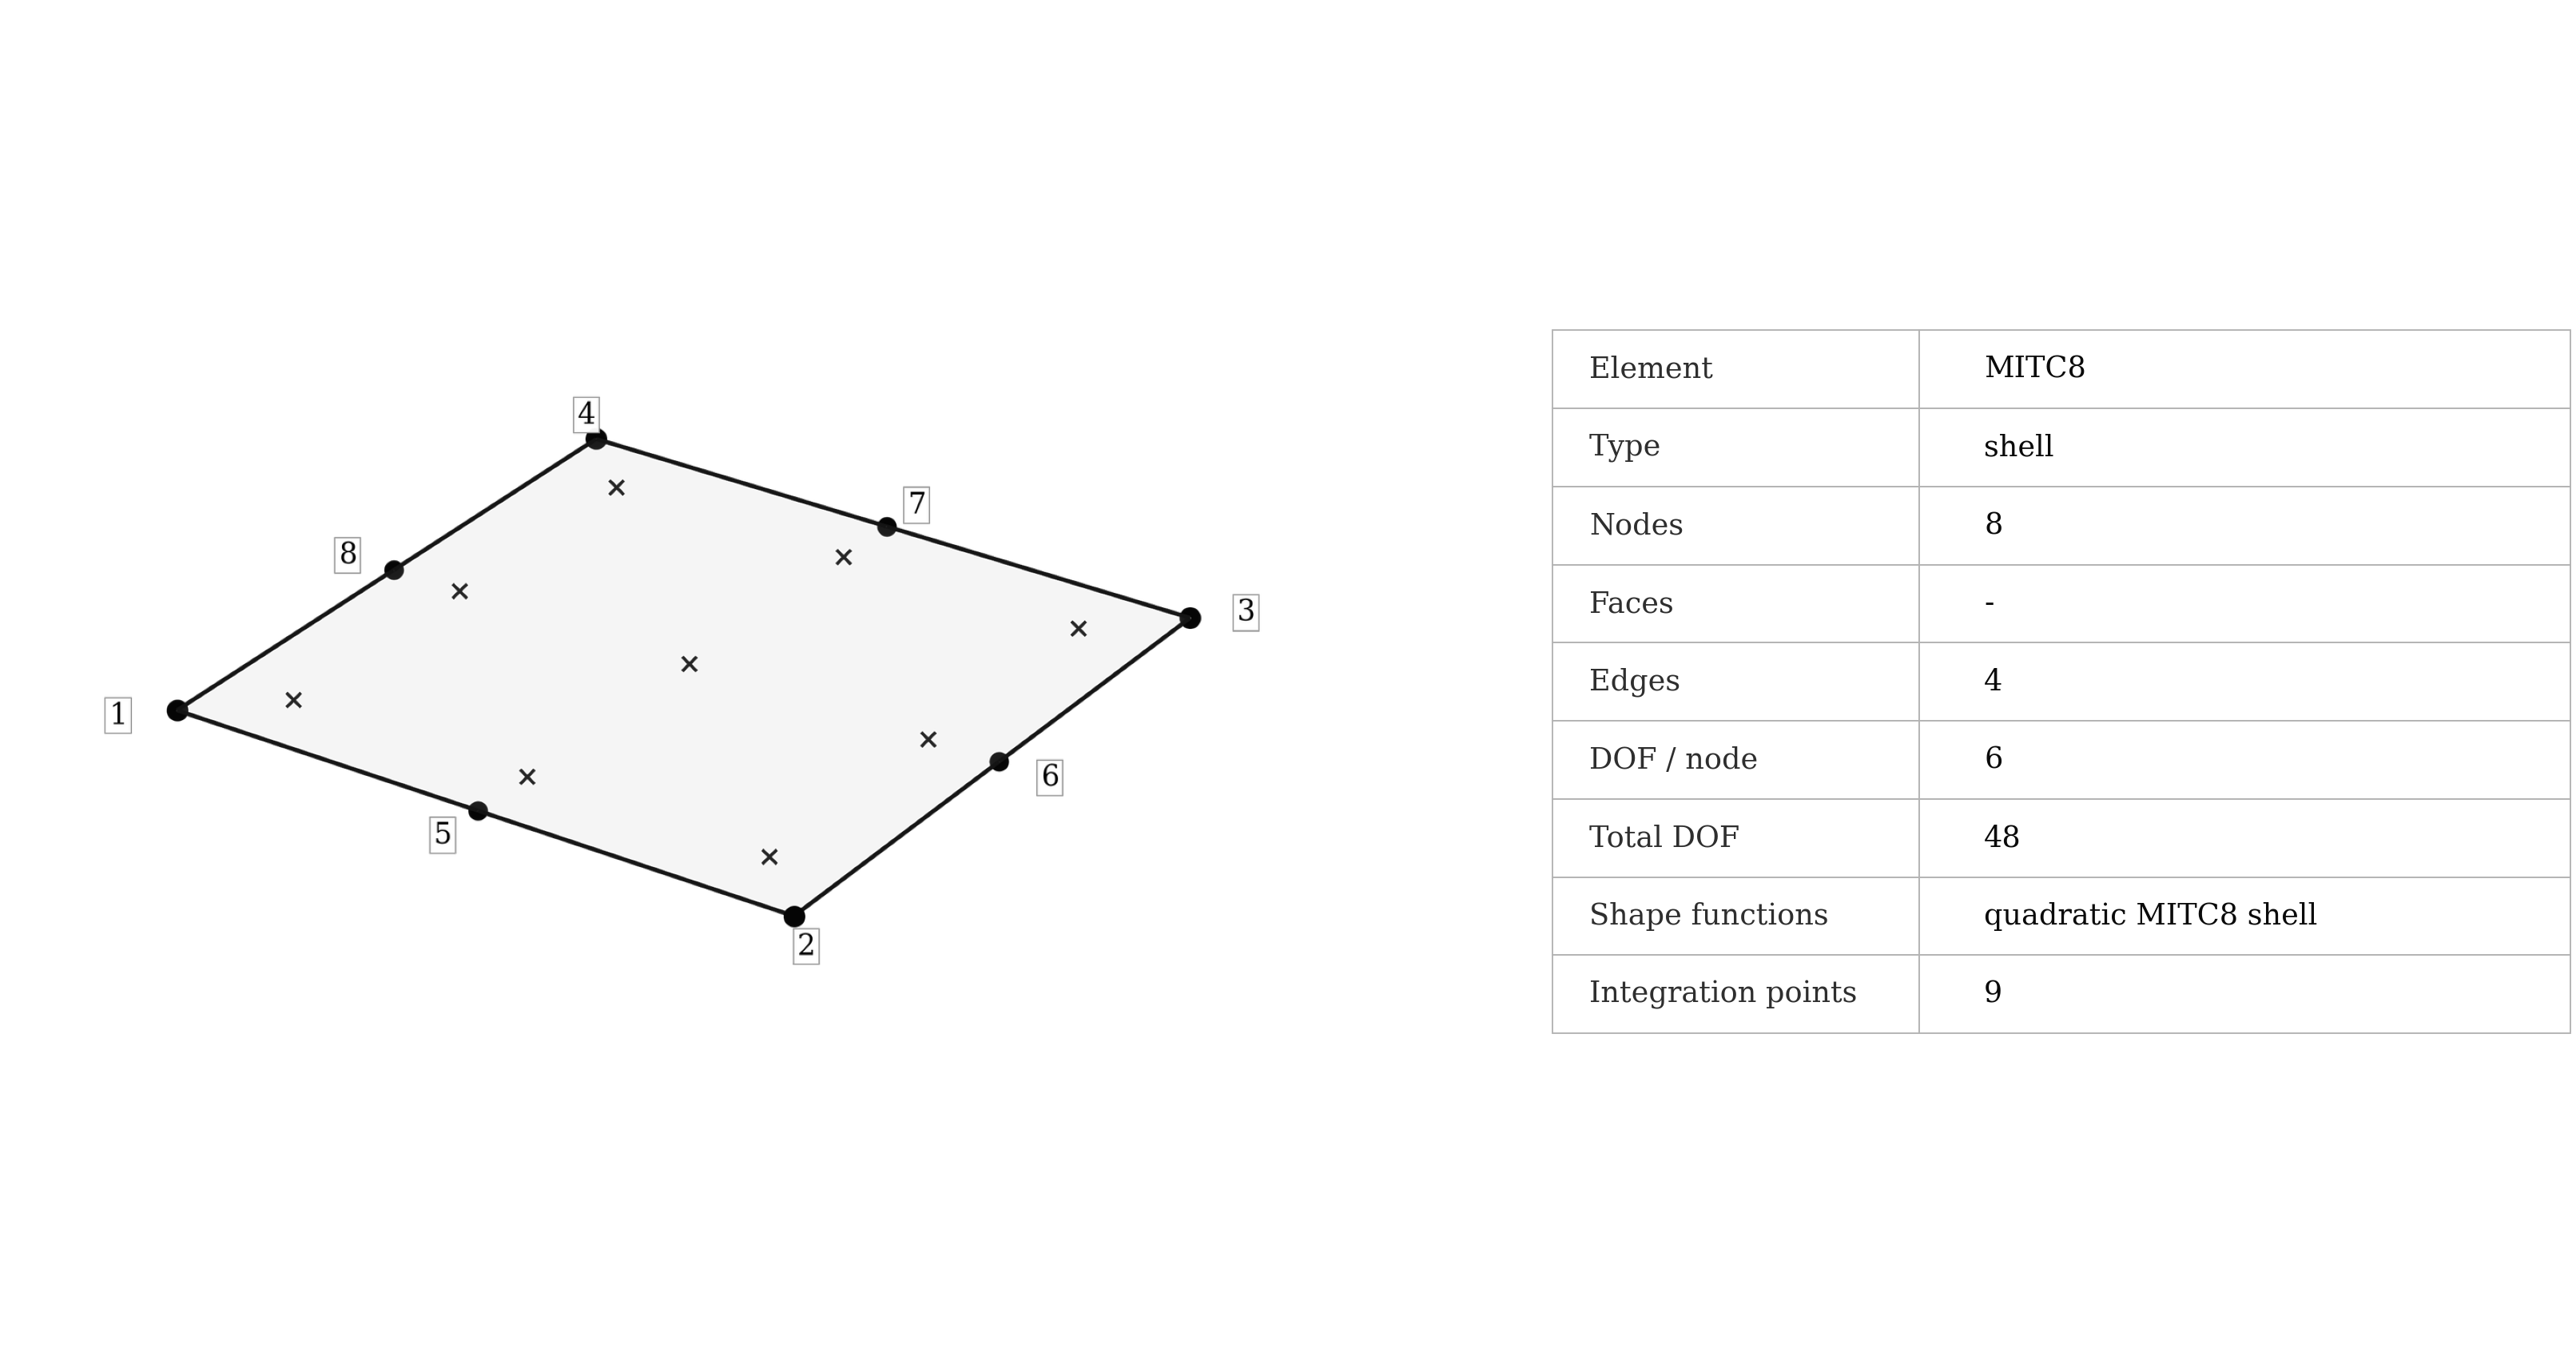
\includegraphics[width=0.80\linewidth]{pages/figures/element_schematics/mitc8_schematic.png}
    \caption{\val{MITC8} quadratic MITC shell.}
\end{figure}

\begin{syntax}
*ELEMENT, TYPE=MITC8, ELSET=<set>
<id>, <n1>, <n2>, <n3>, <n4>, <n5>, <n6>, <n7>, <n8>
\end{syntax}

\val{MITC8} combines the eight-node quadratic quadrilateral topology with MITC-style transverse-shear interpolation. It provides excellent thin-shell bending behaviour in the legacy linear shell family and is useful as a reference formulation for verifying lower-order shell results.

Because the interpolation is quadratic, a regular \val{MITC8} mesh can reproduce smooth bending fields with relatively few elements. The cost per element is higher than for \val{MITC4}, and distorted midside geometry can reduce the expected advantage.

For new nonlinear or general-purpose shell models, prefer \val{MITC8FRT}. Use native \val{MITC8} where comparison with legacy linear shell results is specifically required.

\clearpage
\section{\val{MITC8FRT}: finite-rotation 8-node MITC shell}

\begin{figure}[H]
    \centering
    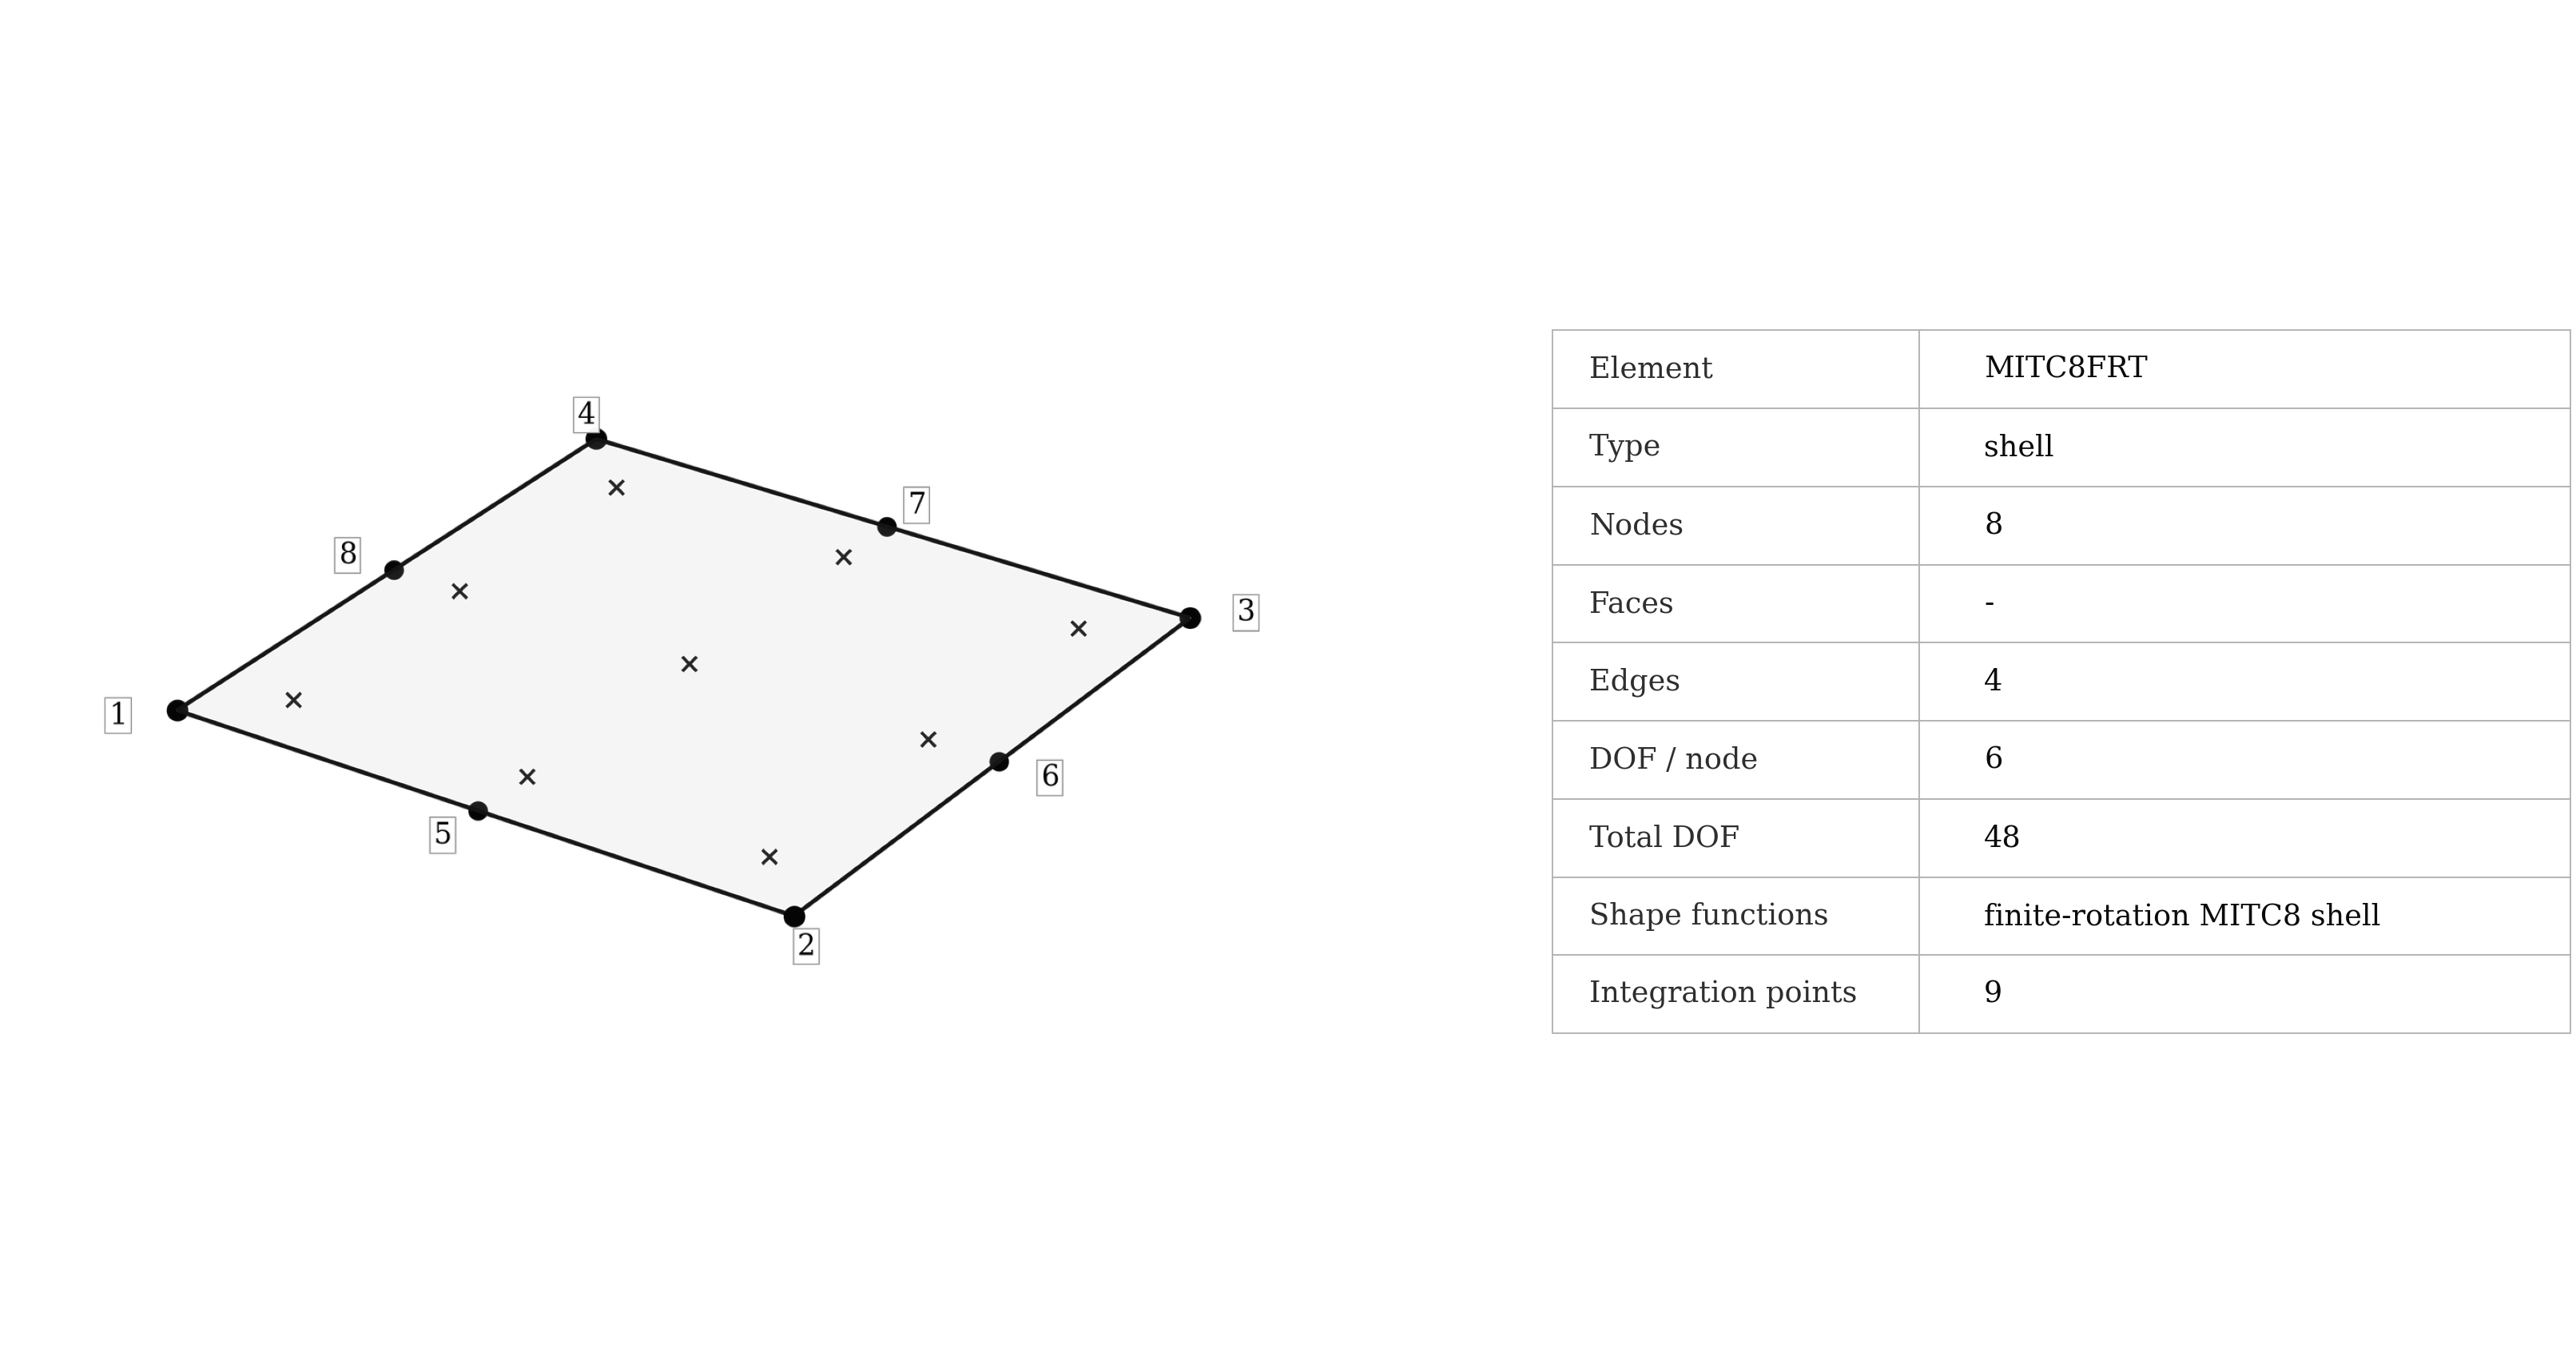
\includegraphics[width=0.80\linewidth]{pages/figures/element_schematics/mitc8frt_schematic.png}
    \caption{\val{MITC8FRT} finite-rotation eight-node shell.}
\end{figure}

\begin{syntax}
*ELEMENT, TYPE=MITC8FRT, ELSET=<set>
<id>, <n1>, <n2>, <n3>, <n4>, <n5>, <n6>, <n7>, <n8>
\end{syntax}

\val{MITC8FRT} is the recommended higher-order quadrilateral shell. It combines an eight-node midsurface interpolation with finite-rotation shell kinematics and MITC transverse-shear treatment. It is intended for accurate bending and curved-shell modelling where the additional interpolation order is worth the increased element cost.

The formulation is especially useful when a curved shell geometry can be represented with a clean quadratic quadrilateral mesh. Compared with a low-order shell, fewer elements may be required to describe smooth curvature and stress-resultant gradients.

Higher order does not make the formulation insensitive to distortion. Warped quadrilaterals, poorly placed midside nodes, inconsistent normals, and abrupt mesh transitions can still produce misleading stiffness and result recovery. Large-rotation models should be checked with deformation-shape inspection and mesh refinement.

Both Abaqus \val{S8} and \val{S8R} are translated to \val{MITC8FRT}.

\clearpage
\section{\val{QSPT}: quadrilateral shear-panel element}

\begin{figure}[H]
    \centering
    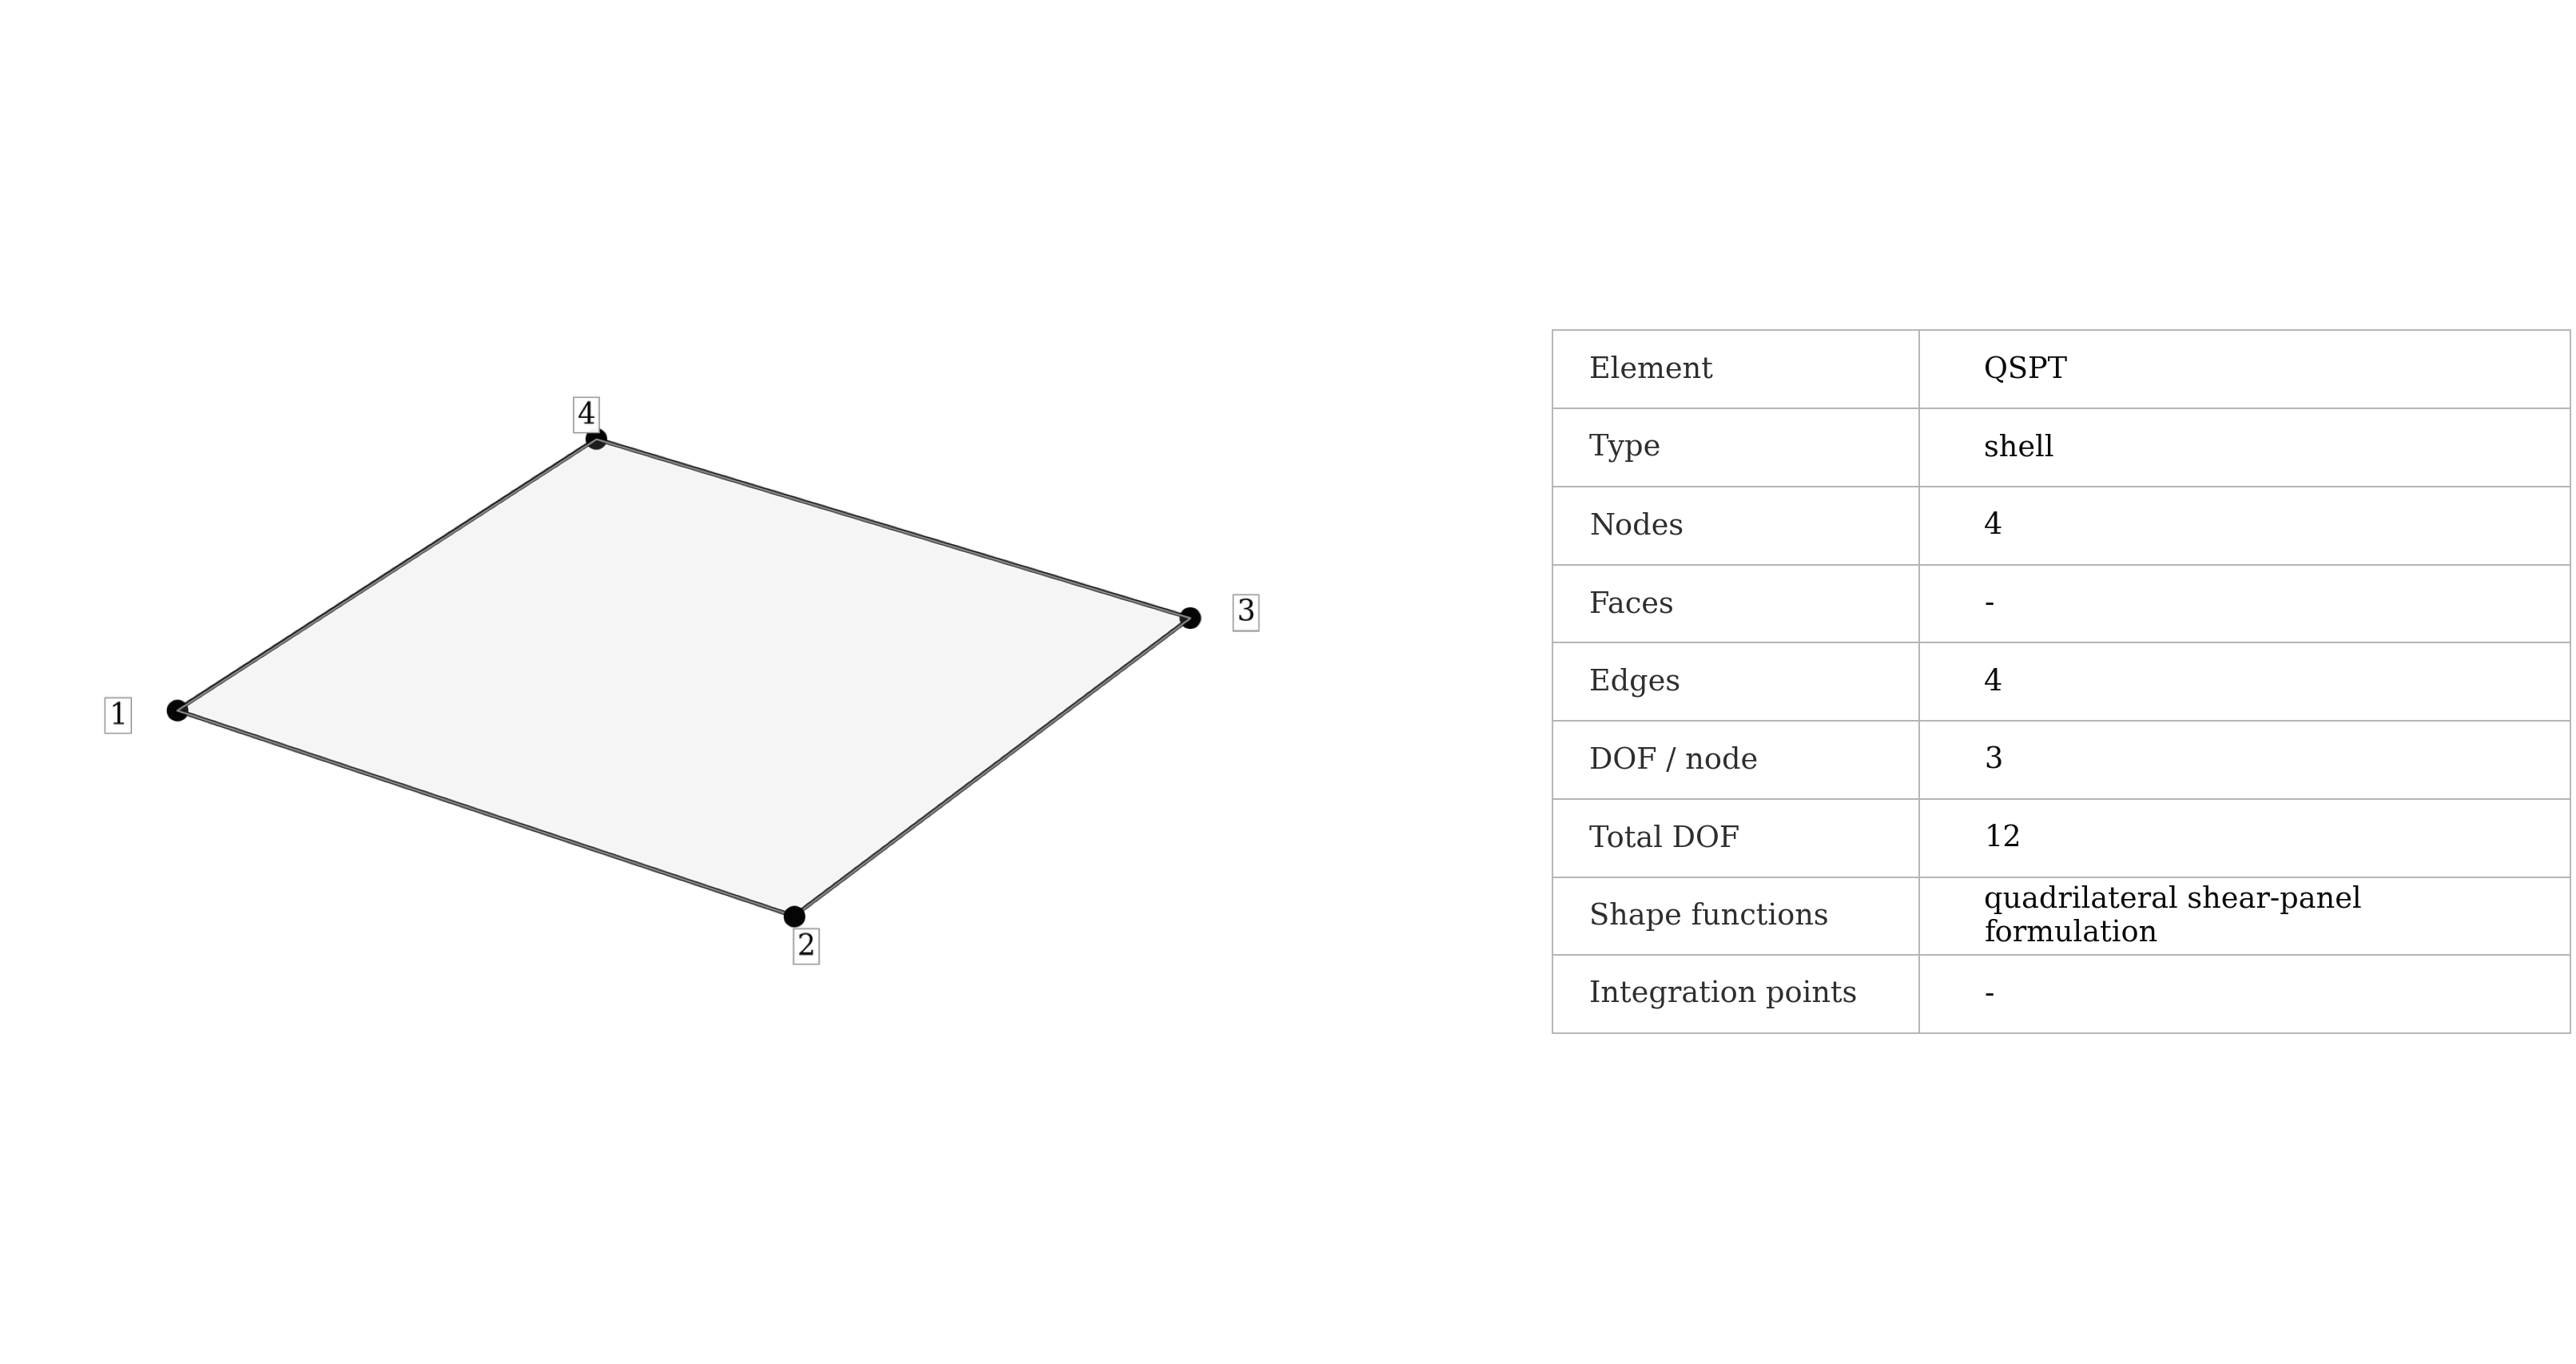
\includegraphics[width=0.78\linewidth]{pages/figures/element_schematics/qspt_schematic.png}
    \caption{\val{QSPT} shear-panel element.}
\end{figure}

\begin{syntax}
*ELEMENT, TYPE=QSPT, ELSET=<set>
<id>, <n1>, <n2>, <n3>, <n4>
\end{syntax}

\val{QSPT} is a specialized four-node quadrilateral panel element developed for shear-flow-oriented structural idealizations. It is intended for simplified panel models where the principal purpose of the element is to transfer in-plane shear rather than reproduce the complete behaviour of a general shell.

Typical applications are preliminary thin-walled structures, webs, aircraft-style shear panels, and reduced-order structural models in which panel shear flow is the primary quantity of interest. In such models \val{QSPT} can provide a compact load-path representation without introducing a complete shell formulation for every panel.

Do not use \val{QSPT} merely because the mesh contains four-node quadrilaterals. It is not a general replacement for \val{MITC4FRT}. If bending stiffness, local shell curvature, full shell resultants, or detailed top/bottom stresses are required, use a shell formulation instead.

\section{Beam and truss elements}

Line elements idealize slender three-dimensional members by describing the cross-section through section properties instead of meshing it explicitly. This can reduce the number of degrees of freedom by orders of magnitude compared with shell or solid modelling. The trade-off is that local three-dimensional connection behaviour, detailed cross-section distortion, holes, welds, and local stress concentrations are not resolved.

\clearpage
\section{\val{B33}: 3D beam element}

\begin{figure}[H]
    \centering
    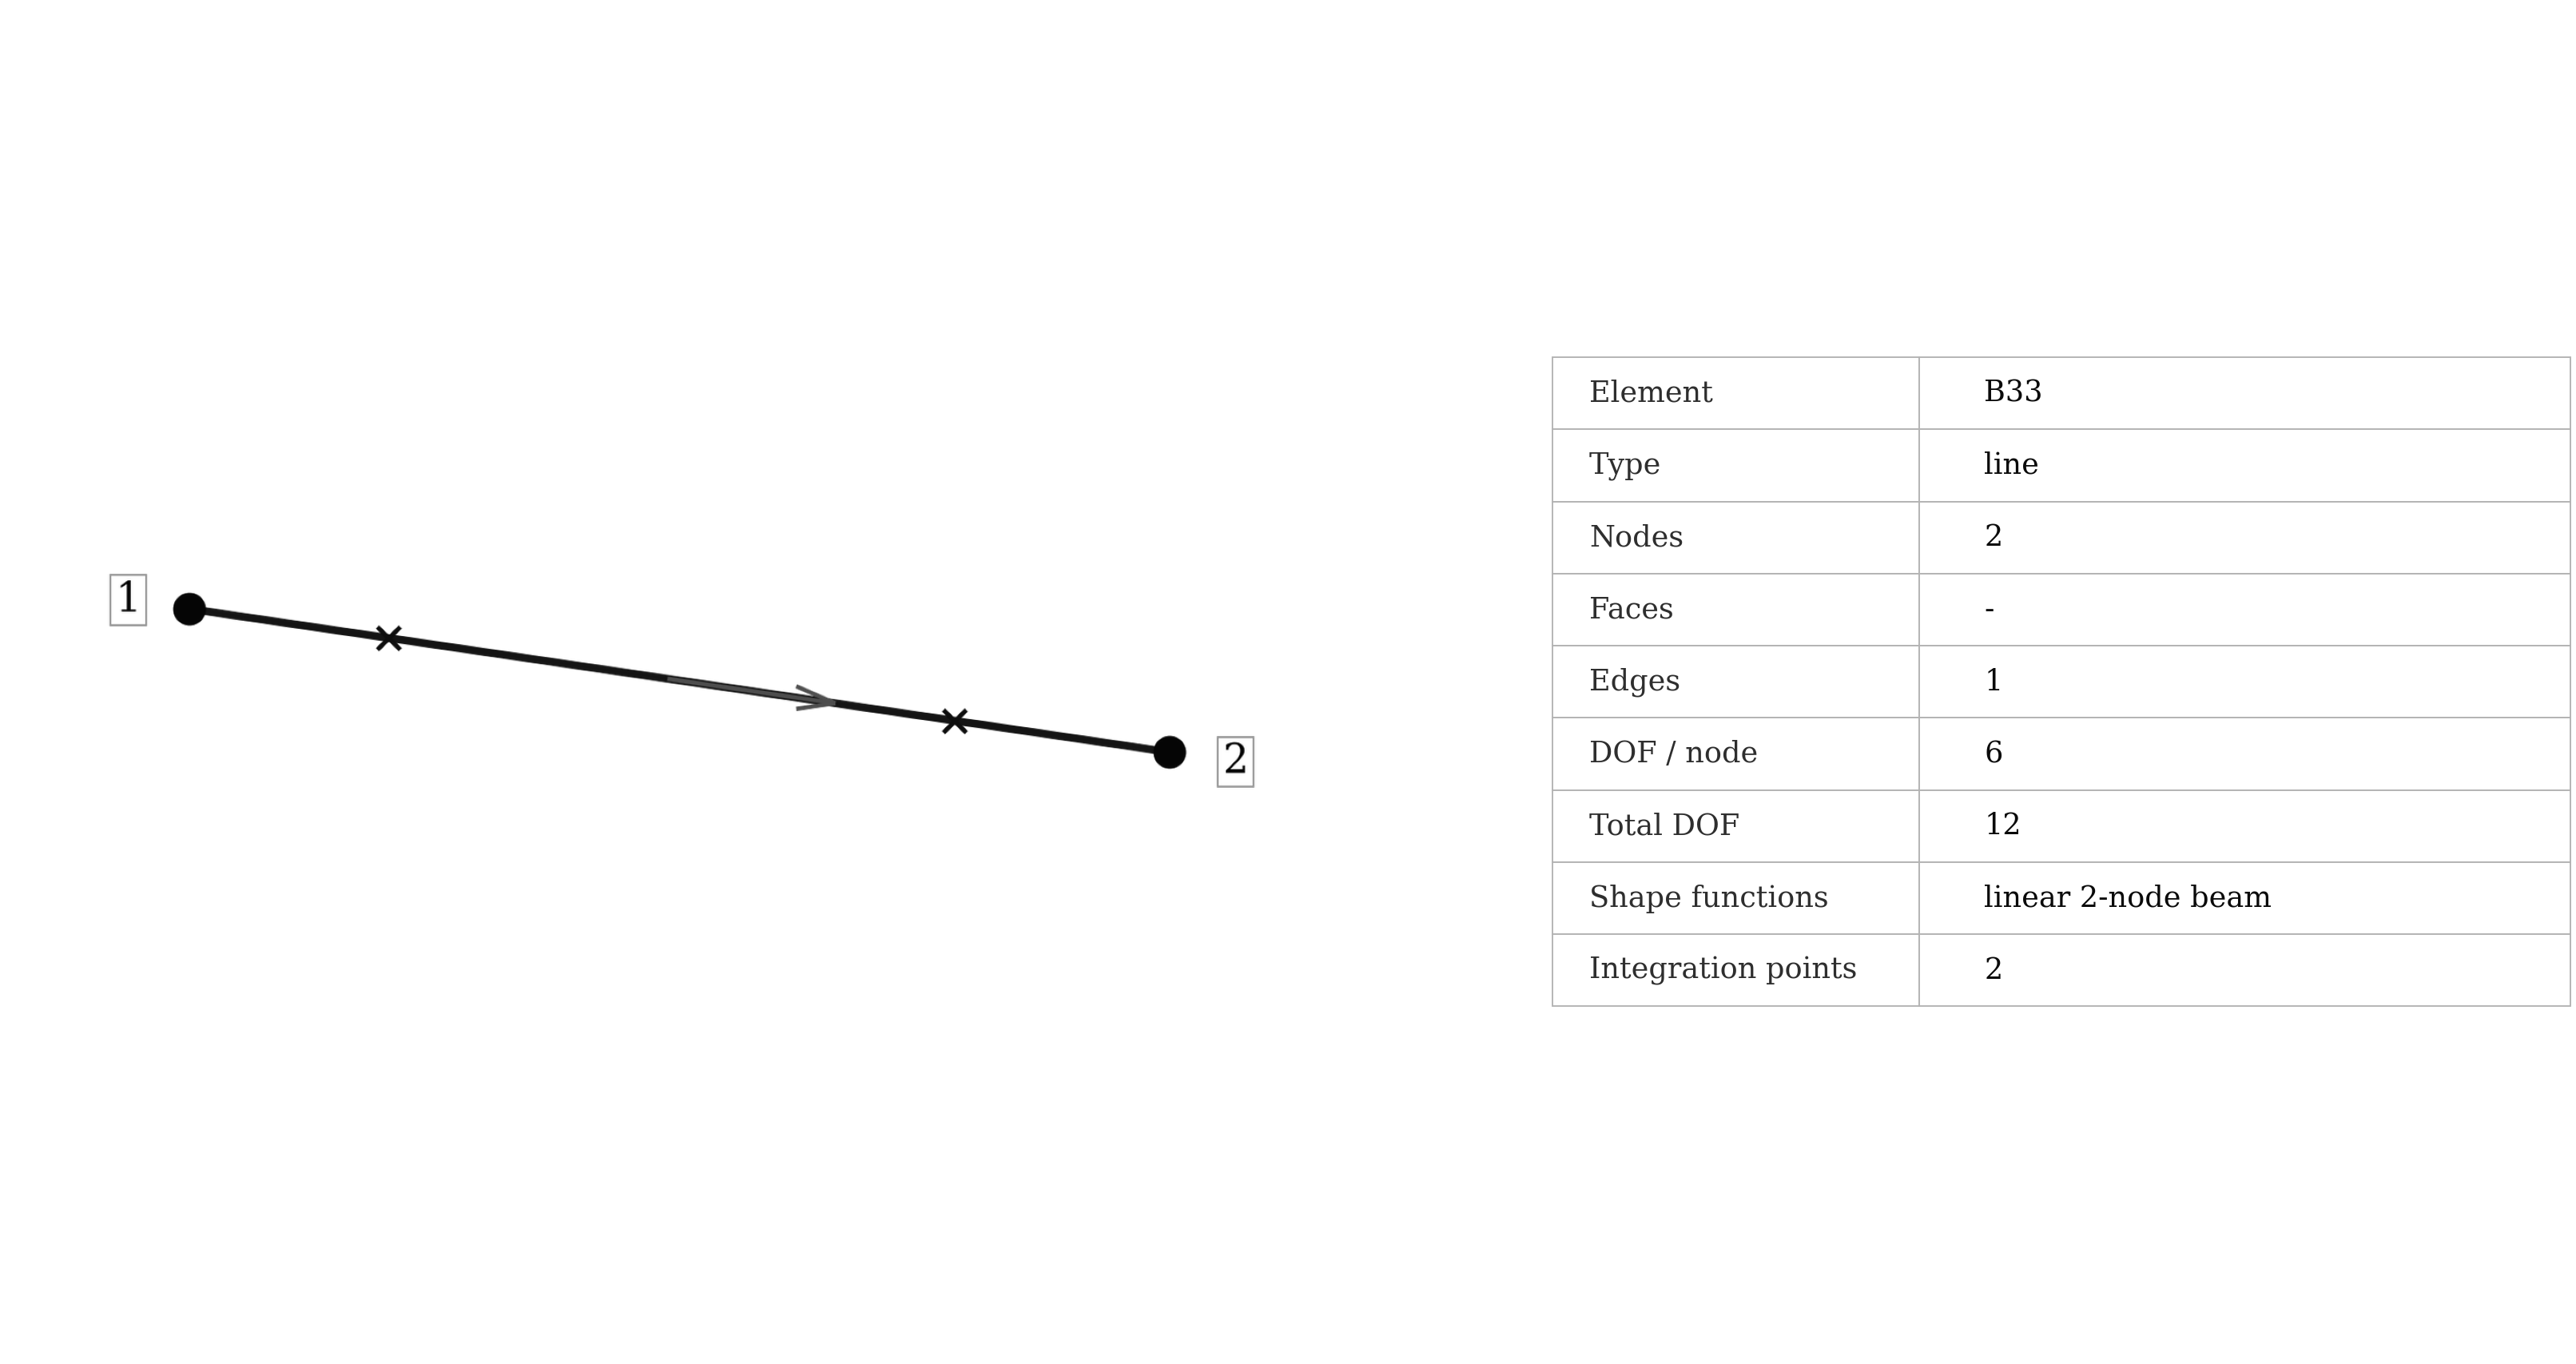
\includegraphics[width=0.70\linewidth]{pages/figures/element_schematics/b33_schematic.png}
    \caption{\val{B33} beam element.}
\end{figure}

\begin{syntax}
*ELEMENT, TYPE=B33, ELSET=<set>
<id>, <n1>, <n2>
\end{syntax}

\val{B33} is a two-node three-dimensional beam element with translational and rotational nodal degrees of freedom. It represents axial deformation, bending, torsion, and the section response defined by \cmd{BEAM SECTION} and the referenced \cmd{PROFILE}.

The current \cmd{ELEMENT} syntax uses exactly two connectivity nodes for \val{B33}. Beam cross-section orientation is supplied by the orientation vector in \cmd{BEAM SECTION}; an additional orientation node is not part of the current connectivity grammar.

Beam elements are appropriate for slender frames, stiffeners, spars, ribs, idealized support members, and other structures where section forces and global deformation are the main engineering quantities. They permit axial area, bending inertias, torsional stiffness, product of inertia, section offsets, and reference-line offsets to be represented without meshing the full cross-section.

The beam idealization does not resolve local connection stresses, bolt or weld geometry, detailed cross-section deformation, or three-dimensional load introduction. Use shells or solids when those local effects determine the design result. Always verify the beam local axes because bending moments, section forces, and profile properties are interpreted in that local system.

The supported Abaqus reader accepts \val{B33} with the same two-node connectivity.

\clearpage
\section{\val{T3}: 2-node truss element}

\begin{figure}[H]
    \centering
    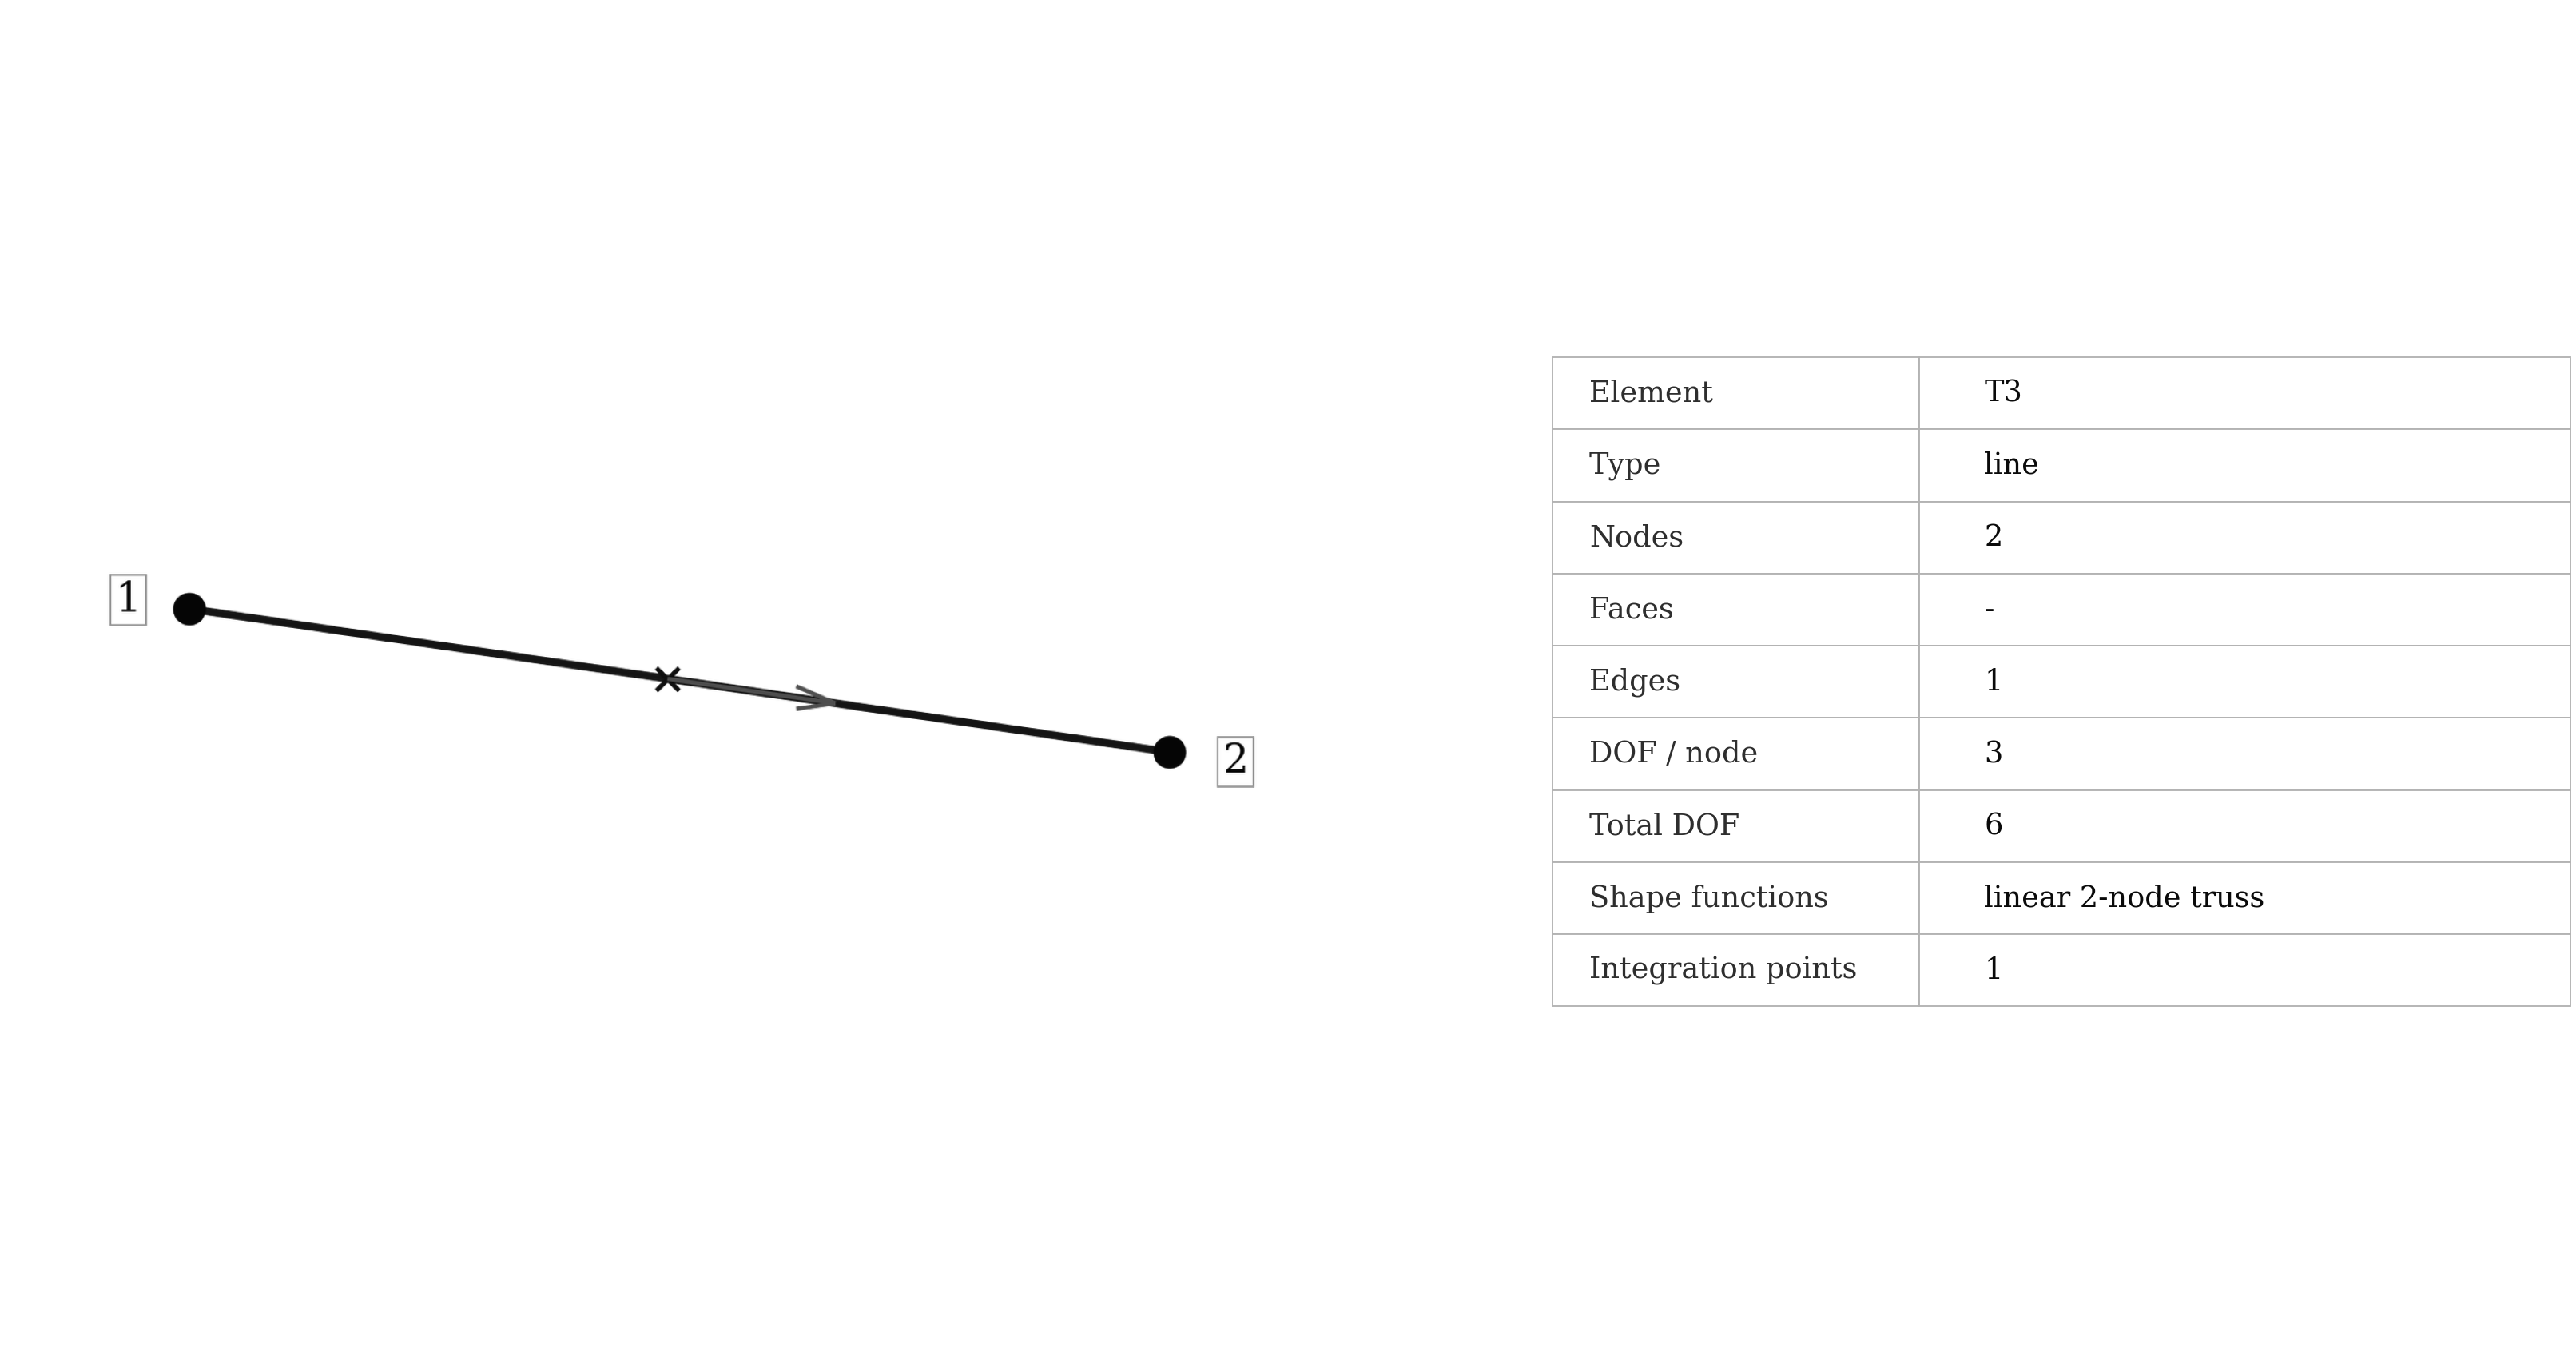
\includegraphics[width=0.68\linewidth]{pages/figures/element_schematics/t3_schematic.png}
    \caption{\val{T3} truss element.}
\end{figure}

\begin{syntax}
*ELEMENT, TYPE=T3, ELSET=<set>
<id>, <n1>, <n2>
\end{syntax}

\val{T3} is a two-node truss element. It carries axial force along its current line direction and uses translational nodal degrees of freedom. The material and cross-sectional area are assigned by \cmd{TRUSS SECTION}.

The element is appropriate for pin-jointed members, rods, braces, links, and other components whose intended structural action is axial tension or compression. Truss models are inexpensive and easy to interpret because the principal mechanical quantities are axial force, axial strain, and axial stress.

The limitations are deliberate. \val{T3} has no bending stiffness, no torsional stiffness, and no rotational continuity. It cannot model fixed-end moments, eccentric frame action, or transverse stiffness of a physical beam. If a member is expected to carry moment, use \val{B33} or a shell/solid representation.

In Abaqus input the corresponding accepted type is \val{T3D2}. The two labels select the same FEMaster truss formulation through their respective input dialects.

\section{Element selection guidelines}

No element is universally best. The following rules are useful starting points:
\begin{itemize}
  \item use \val{C3D10} rather than \val{C3D4} when tetrahedral stress accuracy matters;
  \item use well-shaped hexahedra when the geometry can be meshed naturally in a structured or swept way;
  \item treat \val{C3D5} as a transition element rather than the preferred bulk discretization;
  \item assess reduced-integration solids by deformation shape and refinement, not only by solver convergence;
  \item use the FRT shell family for new shell models, especially when finite rotations or nonlinear analysis are relevant;
  \item choose shell rather than solid idealization when through-thickness stress is not required and the structure is geometrically thin;
  \item choose beam or truss idealizations only when their one-dimensional kinematic assumptions match the physical member;
  \item verify reactions, deformed shapes, energy trends, and mesh convergence whenever the element choice materially affects the result.
\end{itemize}

A solver can converge accurately to the discrete equations of a poor finite-element model. Element selection and mesh convergence therefore remain modelling responsibilities rather than numerical post-processing details.
